% Notes and solutions


% -------------------------------------------------
% Package imports
% -------------------------------------------------
\documentclass[12pt, a4paper]{article}
\usepackage[utf8]{inputenc}% Input encoding
\usepackage[english]{babel}% Set language to english
\usepackage{graphicx}% For importing graphics
\usepackage{amsthm, amsfonts, amssymb, bm}% All the AMS packages
\usepackage{mathtools}% Fixes a few AMS bugs
\usepackage[expansion=false]{microtype}% Fixes to make typography better
\usepackage{hyperref}% For \href{URL}{text}
\usepackage{fancyhdr}% For fancy headers
\usepackage[sharp]{easylist}% Easy nested lists
\usepackage{parskip}% Web-like paragraphs
\usepackage{multicol}% For multiple columns
\usepackage{tikz-cd}% For diagrams
\usepackage{microtype}
\usepackage{listings}% To include source-code
\usepackage[margin = 2.5cm, includehead]{geometry}% May be used to set margins
\usepackage{nicefrac}% Enables \nicefrac{nom}{denom}
%\usepackage[sc]{mathpazo}% A nice font, alternative to CM
\usepackage{booktabs}
\usepackage{fancyvrb} % fancy verbatim

% -------------------------------------------------
% Package setup
% -------------------------------------------------

\newcommand{\Title}{Solutions to ``Pattern Classification'' by Duda et al.}
\newcommand{\Author}{\texttt{tommyod} @ github}
\newcommand{\listSpace}{-0.5em}% Global list space

\title{\Title}
\author{\Author}

% Shortcuts for sets and other stuff in mathematics
\newcommand{\Q}{\mathbb{Q}}
\newcommand{\R}{\mathbb{R}}
\newcommand{\C}{\mathbb{C}}
\newcommand{\D}{\mathcal{D}}
\newcommand{\F}{\mathcal{F}}
\newcommand{\Y}{\mathcal{Y}}
\newcommand{\Reg}{\mathcal{R}}
\newcommand{\Class}{\mathcal{C}}
\newcommand{\Z}{\mathbb{Z}}
\renewcommand{\sf}[1]{\mathsf{#1}}
\newcommand{\vect}[1]{\bm{#1}}
\newcommand{\norm}[1]{\left\lVert#1\right\rVert}
\newcommand{\abs}[1]{\left\lvert#1\right\rvert}

% Shortcuts for probability distributions
\DeclareMathOperator{\N}{\mathcal{N}}
\DeclareMathOperator{\Bern}{\operatorname{Bern}}
\DeclareMathOperator{\Beta}{\operatorname{Beta}}
\DeclareMathOperator{\Bin}{\operatorname{Bin}}
\DeclareMathOperator{\St}{\operatorname{St}}
\DeclareMathOperator{\U}{\operatorname{U}}
\DeclareMathOperator{\KL}{\operatorname{KL}}

% Shortcuts for statistical operators
\DeclareMathOperator{\E}{\mathbb{E}}
\DeclareMathOperator{\var}{\operatorname{var}}
\DeclareMathOperator{\cov}{\operatorname{cov}}
\DeclareMathOperator{\SD}{\operatorname{SD}}
\renewcommand{\H}{\operatorname{H}}



% Change the section command to inluce lines, save space, etc.
%\usepackage{titlesec}
%\titlespacing\subsection{0pt}{6pt plus 4pt minus 2pt}{-0.8em plus 4pt minus 2pt}
%\titlespacing\paragraph{0pt}{6pt plus 4pt minus 2pt}{8pt plus 4pt minus 2pt}
%\titleformat{\section}
%{\normalfont\Large\bfseries}{\thesection}{0em}{$\vartriangleright$ }[{\titlerule[1.2pt]}]

% -------------------------------------------------
% Document start
% -------------------------------------------------
\begin{document}
\maketitle
\begin{abstract}
	
This document contains solutions to selected exercises from the book ``Pattern Recognition'' by Richard O. Duda, Peter E. Hart and David G. Stork.
Although it was written in 2001, the second edition has truly stood the test of time---it's a much-cited, well-written introductory text to the exciting field of \emph{pattern recognition}(or simply \emph{machine learning}).
At the time of writing, the book has close to 40 000 citations according to Google.

While short chapter summaries are included in this document, they are not intended to substitute the book in any way.
The summaries will largely be meaningless without the book, which I recommend buying if you're interested in the subject.

The solutions and notes were typeset in \LaTeX{} to facilitate my own learning process.
Machine learning has rightfully garnered considerable attention in recent years, and while many online resources are worthwhile it seems reasonable to favor books when attempting to learn the material thoroughly. 

I hope you find my solutions helpful if you are stuck. 
Remember to make an attempt at solving the problems yourself before peeking.
More likely than not, the solutions can be improved by a reader such as yourself. 
If you would like to contribute, please submit a pull request at \url{https://github.com/tommyod/lml/}.

\begin{figure}[ht!]
	\centering
	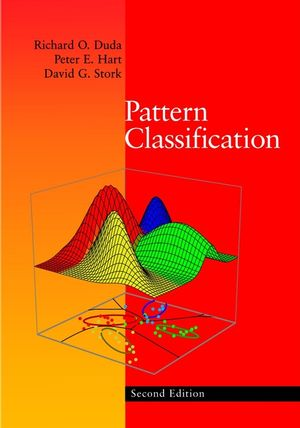
\includegraphics[width=0.30\linewidth]{figs/duda}
	\caption{The front cover of \cite{duda_pattern_2000}.}
	\label{fig:duda1}
\end{figure}
\end{abstract}

\clearpage
\tableofcontents
\clearpage
\section{Notes from ``Pattern Classification''}
\setcounter{subsection}{1}
\subsection{Bayesian Decision Theory}
\begin{easylist}[itemize]
\ListProperties(Space=\listSpace, Space*=\listSpace, Numbers1=l, FinalMark1={)})
# Bayes theorem is
\begin{equation*}
	P(\omega_j \mid \vect{x}) = \frac{p(\vect{x} \mid \omega_j) \times P(\omega_j)}{p(\vect{x})}
	= \frac{\text{likelihood} \times \text{prior}}{\text{evidence}}.
\end{equation*}
The Bayes decision rule is to choose the state of nature $\omega_m$ such that
\begin{equation*}
	\omega_m = \arg \max_j P(\omega_j \mid \vect{x}).
\end{equation*}

# Loss functions (or risk functions) with losses other than zero-one are possible.
 In general, we choose the action $\lambda$ to minimize the risk $R(\lambda \mid \vect{x})$.
 
# The multivariate normal density (the Gaussian) is given by
\begin{equation*}
	p(\vect{x} \mid \vect{\mu}, \vect{\Sigma}) = \frac{1}{(2 \pi)^{d/2} \abs{\vect{\Sigma}}^{1/2}} 
	\exp \left[ - \frac{1}{2} 
	\left( \vect{x} - \vect{\mu} \right)^T \vect{\Sigma}^{-1} 
	\left( \vect{x} - \vect{\mu} \right) \right].
\end{equation*}
It is often analytically tractable, and closed form discriminant functions exist.

# If features $\vect{y}$ are missing, we integrate them out (marginalize) using the sum rule
\begin{equation*}
	p(\vect{x}) = \int p(\vect{x}, \vect{y}) \, d\vect{y} = \int p(\vect{x} \mid \vect{y}) p(\vect{y}) \, d\vect{y}.
\end{equation*}

# In Bayesian belief networks, influences are represented by a directed network.
If $B$ is dependent on $A$, we add a directed edge $A \to B$ to the network.
\end{easylist}
\begin{figure}[ht!]
\centering
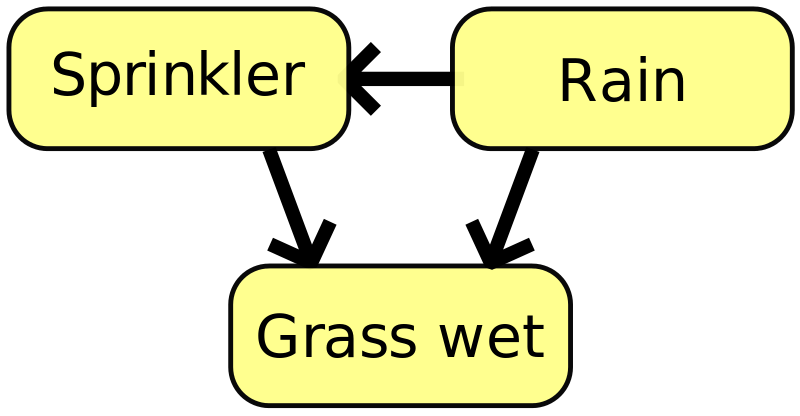
\includegraphics[width=0.3\linewidth]{figs/bayesian_belief_network}
\caption{A Bayesian belief network. The source is Wikipedia.}
\label{fig:bayesian_belief_network}
\end{figure}




\subsection{Maximum-likelihood and Bayesian parameter estimation}
\begin{easylist}[itemize]
\ListProperties(Space=\listSpace, Space*=\listSpace, Numbers1=l, FinalMark1={)})
# The \emph{maximum likelihood} of a distribution $p(\vect{x} \mid \vect{\theta})$ is given by $\hat{\vect{\theta}} = \arg \max_{\vect{\theta}} p(\D \mid \vect{\theta})$,
assuming i.i.d. data points and maximizing the log-likelihood, we have
\begin{equation*}
	\hat{\vect{\theta}} = \arg \max_{\vect{\theta}} \ln  p(\D \mid \vect{\theta}) = \arg \max_{\vect{\theta}}  \ln  \prod_{i=1}^{n} p(\vect{x}_i \mid \vect{\theta})  .
\end{equation*}
Analytical solutions exist for the Gaussian, but in general a maximum likelihood estimate may be biased, in the sense that $\E_x[ \hat{\vect{\theta}} ] = \int \hat{\vect{\theta}} p(\vect{x}) \, d\vect{x} \neq \vect{\theta}$.

# In the Bayesian framework, the parameter $\vect{\theta}$ is expressed by a probability density function $p(\vect{\theta})$.
This is called the \emph{prior} distribution of $\vect{\theta}$, which is updated when new data is observed.
The result is called the \emph{posterior} distribution, given by
\begin{equation*}
	p(\vect{\theta} \mid \D)  
	= 
	\frac{p(\D \mid \vect{\theta}) p (\vect{\theta})}
	{p(\D)}
	= 
	\frac{p(\D \mid \vect{\theta}) p (\vect{\theta})}
	{\int p(\D \mid \vect{\theta}) p(\vect{\theta}) \, d \vect{\theta}}.
\end{equation*}
The estimate of $\vect{x}$ then becomes
\begin{equation*}
	p(\vect{x} \mid \D) = \int p(\vect{x}, \vect{\theta} \mid \D) \, d\vect{\theta} =
	\int p(\vect{x} \mid \vect{\theta} , \D) p(\vect{\theta} \mid \D)  \, d\vect{\theta} =
	\int p(\vect{x} \mid \vect{\theta}) p(\vect{\theta} \mid \D)  \, d\vect{\theta},
\end{equation*}
which may be interpreted as a weighted average of models $p(\vect{x} \mid \vect{\theta})$, where $p(\vect{\theta} \mid \D)$ is the weight associated with the model.

# The Bayesian framework is analytically tractable when using Gaussians.
For instance, we can compute $p(\vect{\mu} \mid \D)$ if we assume $p(\vect{\mu}) \sim \N(\vect{\mu}_0, \vect{\Sigma}_0)$.
The distribution $p(\vect{\mu})$ is called the \emph{conjugate prior} and $p(\vect{\mu} \mid \D)$ is a \emph{reproducing density}, since the normal prior transforms to a normal posterior (with different parameters) when new data is observed.

# In summary the Bayesian framework allows us to incorporate prior information, but the maximum-likelihood approach is simpler.
Maximum likelihood gives us an estimate $\hat{\vect{\theta}}$, but the Bayesian framework gives us $p(\vect{\theta}  \mid  \D)$---the full distribution.

# Principal Component Analysis (PCA) yields components useful for \emph{representation}.
The covariance matrix is diagonalized, and low-variance directions in the hyperellipsoid are eliminated.
The computation is performed using the SVD.

# Discriminant Analysis (DA) projects to a lower dimensional subspace with optimal \emph{discrimination} (and not representation).

# Expectation Maximization (EM) is an iterative algorithm for finding the maximum-likelihood when data is missing (or latent).

\begin{figure}[ht!]
	\centering
	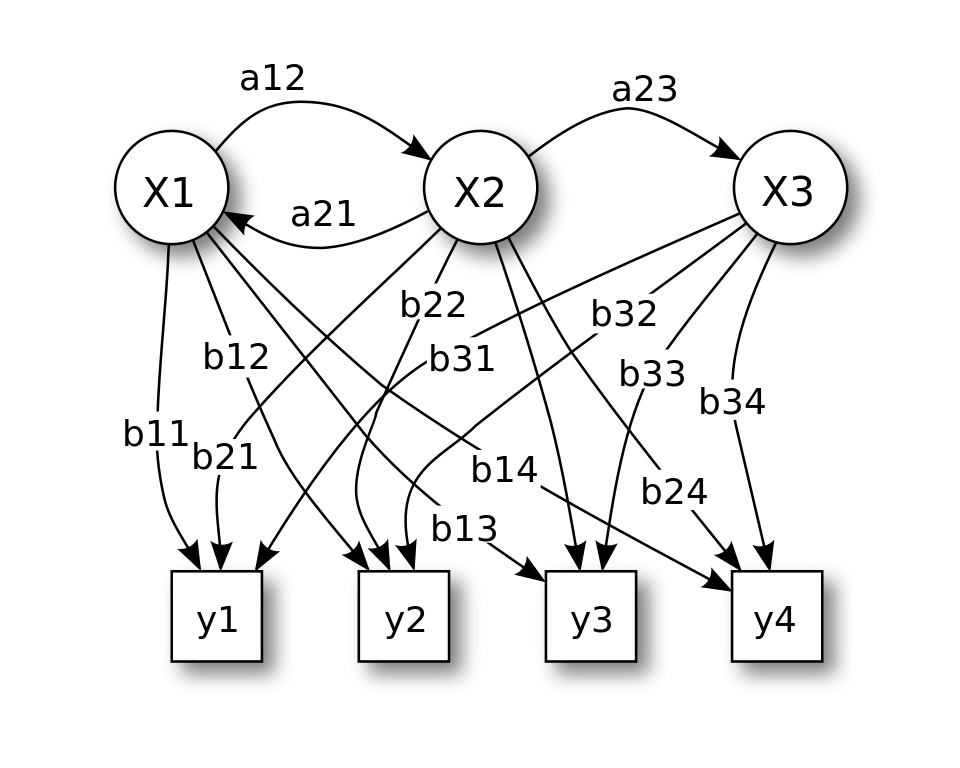
\includegraphics[width=0.45\linewidth]{figs/hidden_markov}
	\caption{A hidden Markov model. The source is Wikipedia.}
	\label{fig:hidden_markov}
\end{figure}

# A discrete, first order, hidden Markov model consists of a transition matrix $\vect{A}$ and an emission matrix $\vect{B}$.
The probability of transition from state $i$ to state $j$ is given by $a_{ij}$, and the probability that state $i$ emits signal $j$ is given by $b_{ij}$.
Three fundamental problems related to Markov models are:
## The evaluation problem - probability that $\vect{V}^T$ was emitted, given $\vect{A}$ and $\vect{B}$.
## The decoding problem - determine most likely sequence of hidden states $\vect{\omega}^T$, given emitted $\vect{V}^T$, $\vect{A}$ and $\vect{B}$.
## The learning problem - determine $\vect{A}$ and $\vect{B}$ given training observations of $\vect{V}^T$ and a coarse model.



\end{easylist}




\subsection{Nonparametric techniques}
\begin{easylist}[itemize]
\ListProperties(Space=\listSpace, Space*=\listSpace, Numbers1=l, FinalMark1={)})
# Two conceptually different approaches to nonparametric pattern recognition are: 
## Estimation of densities $p(\vect{x} \mid w_j)$, called the \emph{generative} approach.
## Estimation of $P(w_j \mid \vect{x})$, called the \emph{discriminative} approach.

# Parzen-windows (kernel density estimation) is a generative method. 
It places a \emph{kernel function} $\phi: \R_+ \to \R_+$ on every data point $\vect{x}_i$ to create a density estimate
\begin{equation*}
	p_n(\vect{x}) = \frac{1}{n} \sum_{i=1}^{n} \frac{1}{V_n} 
	\phi \left( \frac{\norm{\vect{x} - \vect{x}_i}_p}{h_n}  \right),
\end{equation*}
where $\norm{\cdot}_p: \R^d \to \R_+$ is the $p$-norm (which induces the so-called \emph{Minkowski metric}) and $h_n \geq 0$ is the bandwidth.

# $k$-nearest neighbors is a discriminative method.
It uses information about the $k$ nearest neighbors of a point $\vect{x}$ to compute $P(w_j \mid \vect{x})$.
This automatically uses more of the surrounding space when data is sparse, and less of the surrounding space when data is dense.
The $k$-nearest neighbor estimate is given by
\begin{equation*}
	P(w_j \mid \vect{x}) = \frac{\text{\# samples labeled } w_j}{k}.
\end{equation*}

# The \emph{nearest neighbor method} uses $k= 1$.
It can be shown that the error rate $P$ of the nearest neighbor method is never more than twice the Bayes error rate $P^*$ in the limit of infinite data.
More precisely, we have $P^* \leq P \leq P^* (2 - \frac{c}{c-1} P^*)$.

# In some applications, careful thought must be put into metrics.
Examples include periodic data on $\R / \Z$ and image data where the metric should be invariant to small shifts and rotations.
One method to alleviate the problems of using the 2-norm as a metric on images is to introduce the \emph{tangent distance}.
For an image $\vect{x}'$, the tangent vector of a transformation $\F$ (such as rotation by an angle $\alpha_i$) is given by
\begin{equation*}
	\vect{TV}_i = \F\left(\vect{x}'; \alpha_i \right) - \vect{x}'.
\end{equation*}
If several transformations are available, their linear combination may be computed.
For each test point $\vect{x}$, we search the tangent space for the linear  combination minimizing the metric.
This gives a metric $D(\vect{x}, \vect{x}')$ which is more invariant to transformations such as small rotations and translations, compared to the 2-norm.

# \emph{Reduced Coloumb energy networks} use ideas from both Parzen windows and $k$-nearest neighbors.
It adjusts the size of the window so that it is less than some maximal radius, while not touching any observation of a different class.
This creates ``basins of attraction'' for classification.
\end{easylist}



\subsection{Linear discriminant functions}
\begin{easylist}[itemize]
\ListProperties(Space=\listSpace, Space*=\listSpace, Numbers1=l, FinalMark1={)})
# Linear discriminant functions split the feature space in two with a hyperplane.
The equation for a hyperplane is given by
\begin{equation*}
	g(\vect{x}) = \vect{\omega}^T \vect{x} + \omega_0 = \vect{a}^T \vect{y} =
	\begin{pmatrix}
	\omega_0 & \vect{\omega}
	\end{pmatrix}
	\begin{pmatrix}
	1 \\
	\vect{x}
	\end{pmatrix},
\end{equation*}
where $\omega_0$ is the bias. 
The form $\vect{a}^T \vect{y}$ is called the \emph{augmented} form.

\begin{figure}[ht!]
	\centering
	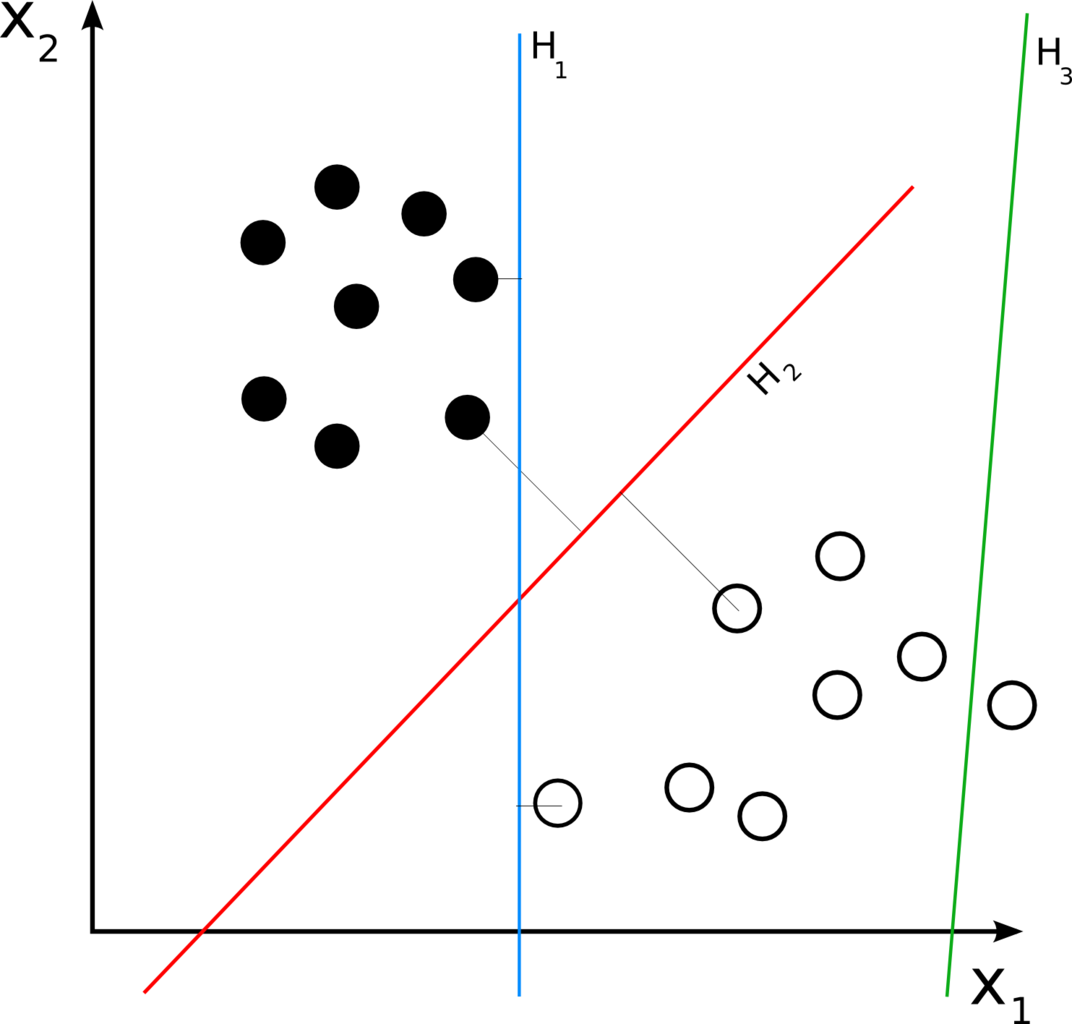
\includegraphics[width=0.35\linewidth]{figs/separating_hyperplanes}
	\caption{Linear discriminant functions. The source is Wikipedia.}
	\label{fig:separating_hyperplanes}
\end{figure}

# A linear machine assigns a point $\vect{x}$ to $\omega_i$ if
\begin{equation*}
	g_i( \vect{x} ) \geq g_j( \vect{x} )
\end{equation*}
for every other class $j$.
This leaves no ambiguous regions in the feature space.

# By introducing mappings $\vect{y} = h(\vect{x})$ to higher- or lower-dimensional spaces, non-linearities in the original $\vect{x}$-space may be captured by linear classifiers working in $\vect{y}$-space. 
An example is $\vect{y} = h(\vect{x}) = \exp(-\vect{x}^T \vect{x})$ if data from one class is centered around the origin.
Another example is transforming periodic data with period $P$ from $0 \leq x < P$ to $\vect{y}$ by use of the functions
\begin{equation*}
	y_1 = \cos \left( 2 \pi x / P \right)
	\qquad 
	y_2 = \sin \left( 2 \pi x / P \right).
\end{equation*}

# Several algorithms may be used to minimize an error function $J(\vect{a})$.
Two popular choices are \emph{gradient descent} and \emph{Newton descent}.
## Gradient descent moves in the direction of the negative gradient.
It is often controlled by a step length parameter $\eta(k)$, which may decrease as the iterations $k$ increase.
The update rule is given by
\begin{equation*}
	\vect{a} \leftarrow \vect{a} - \eta(k) \nabla J(\vect{a}).
\end{equation*}
## Newton descent also moves in the direction of the negative gradient, but the optimal step length is computed by linearizing the function $\nabla J(\vect{a})$ (or, equivalently, a second order approximation of $\vect{a}$).
The update rule is given by
\begin{equation*}
\vect{a} \leftarrow \vect{a} - \vect{H}^{-1} \nabla J(\vect{a}).
\end{equation*}

# Criterion functions for linearly separable data sets include:
## The Perceptron function $\sum_{y \in \Y} (-\vect{a}^T \vect{y})$, which is not smooth.
## The squared error with margin, given by $\sum_{y \in \Y} (\vect{a}^T \vect{y} - b)^2 / \norm{\vect{y}}^a$.

# The \emph{Mean Squared Error} (MSE) approach may be used, but it is not guaranteed to yield a separating hyperplane---even if one exists.
## The MSE solution is found analytically by the pseudoinverse $\vect{A}^\dagger = \left( \vect{A}^T \vect{A} \right)^{-1} \vect{A}^T$. 
The pseudoinverse should never be used explicitly because it's numerically wasteful and unstable.
It represents the analytical solution to the problem
\begin{equation*}
	\min_x \vect{e}^T\vect{e} = 
	\min_x \left(\vect{b} - \vect{A}\vect{x}\right)^T
	\left(\vect{b} - \vect{A}\vect{x}\right),
\end{equation*}
which is solved by $\vect{x} = \vect{A}^\dagger \vect{b}$.
## The MSE approach is related to Fisher's linear discriminant for an appropriate choice of margin vector $\vect{b}$.
## LMS may be computed using matrix procedures (never use the pseudoinverse directly) or by the gradient descent algorithm.
## Ho-Kashyap procedures yield a separating hyperplane if one exists.

# \emph{Linear programming} (LP) may also be used to find a separating hyperplane. Several reductions are possible by introduction of \emph{artificial variables}.
## Minimizing the Perceptron criterion function may be formulated as LP, and the result is decent even if a separating hyperplane does not exist.

# \emph{Support Vector Machines} (SVM) find the minimum margin hyperplane.
This is a quadratic programming (QP) problem, and the dual problem is easier to solve than the primal problem.
\end{easylist}


\subsection{Multilayer Neural Networks}

\begin{figure}[ht!]
\centering
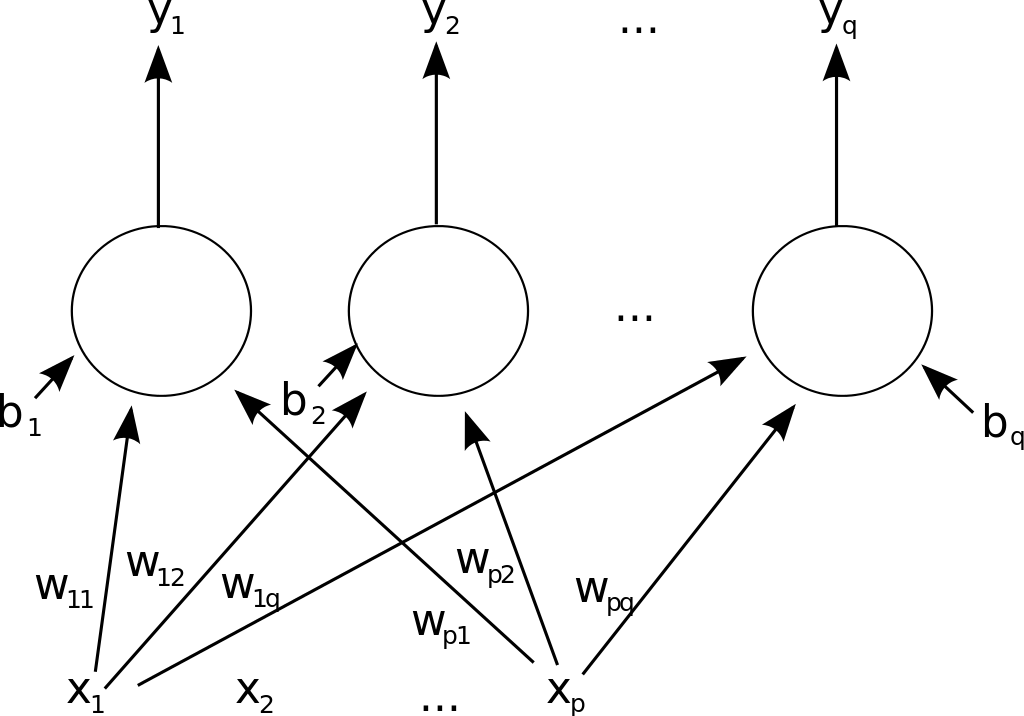
\includegraphics[width=0.45\linewidth]{figs/neuralnet}
\caption{A three-layer neural network with bias. The source is Wikipedia.}
\label{fig:neuralnet}
\end{figure}



\begin{easylist}[itemize]
\ListProperties(Space=\listSpace, Space*=\listSpace, Numbers1=l, FinalMark1={)})
# The feedforward operation on a $d - n_H -c$ three-layer neural network is defined by the following equation for the output
\begin{equation*}
	z_k = f \left( \sum_{j=1}^{n_H} w_{kj} f \left( \sum_{i=1}^{d} w_{ji} x_i + w_{j0} \right) + w_{k0} \right).
\end{equation*}

- The \emph{Kolmogorov-Arnold representation theorem} implies that \emph{any} continuous function from input to output may be expressed by a three layer $d - n_H - c$ neural network with sufficiently many hidden units.

# Backpropagation learns the weights $\vect{w}$ by the gradient descent equation $\vect{w}_{n+1} = \vect{w}_{n} - \eta \nabla J(\vect{w}_{n})$. 
The gradient, or derivative, is found by repeated application of the chain rule of calculus.
Several protocols are available for backpropagation: stochastic, batch and on-line.
## Backpropagation may be thought of as feature mapping.
While the inputs $x_i$ are not necessarily linearly separable, the outputs $y_j$ of the hidden units become linearly separable as the weights are learned.
The final linear discriminant works on this data instead of the $x_i$.

# Practical tips for improving learning in neural networks include:
standardizing features, 
adding noise and data augmentations, 
initializing weights to random values in the range $-1 / \sqrt{d} < w_{ji} < 1 / \sqrt{d}$, 
using momentum in the gradient descent algorithm, 
adding weight decay (equivalent to regularization) while learning, 
training with hints (output units which are subsequently removed) and 
experimenting with various error functions.

# Seconds order methods for learning the weights inluce
## \textbf{Newtons method} -- uses $\vect{H}$ in addition to $\nabla J(\vect{w})$.
## \textbf{Quickprop} -- two evaluations of $\nabla J(\vect{w})$ to approximate a quadratic.
## \textbf{Conjugate gradient descent} -- uses conjugate directions, which consists of a series of line searches. 
A given search direction does not spoil the result of the previous line searches.
This is equivalent to a ``smart momentum.''

# Other networks include:
## Convolutional Neural Networks (CNNs) -- translation invariant, has achieved great success on image data.
## Recurrent Neural Networks (RNNs) -- the output of the previous prediction is fed into the subsequent prediction. 
This simulates ``memory'', and RNNs have been successful on time series data.
## Cascade correlation -- a technique where the topology is altered by adding more units until the performance is sufficiently good.
\end{easylist}







\subsection{Stochastic methods}
\begin{easylist}[itemize]
\ListProperties(Space=\listSpace, Space*=\listSpace, Numbers1=l, FinalMark1={)})
# Stochastic methods are used to search for optimal solutions when techniques such as gradient descent are not viable.
For instance if the model is very complex, has a discrete nature where gradients are not suitable, or if there are time constraints.

# \emph{Simulated annealing} is an optimization technique.
To minimize the error $E(\vect{s})$, where $\vect{s} \in [-1, 1]^n$, we change a random entry of $\vect{s}$.
\begin{easylist}
## If the change produces a better result, then keep the new $\vect{s}$.
## If the change does not produce a better result, we still might keep the change. 
\end{easylist}
The probability of keeping a change which increases the error $E(\vect{s})$ is a function of the temperature $T$, which typically decreases exponentially as the algorithm progresses.
Initially simulated annealing is a \emph{random search}, and as the temperature progresses it becomes a \emph{greedy search}.

# \emph{Deterministic simulated annealing} replaces discrete $s_i$ with analog (continuous) $s_i$.
This forces the other magnets $s_k$ ($k \neq i$) to determine $s_i$
\begin{equation*}
	s_i = f(T, \ell_i) = \tanh \left( \frac{\ell_i}{T} \right).
\end{equation*}
As $T \to 0$, the $\tanh (\cdot)$ sigmoid function converges to a step function.


# \emph{Boltzmann networks} (or Boltzmann machines) employ simulated annealing in a network to make predictions.
First, weights $w_{ij}$ are learned so that inputs $s_j \in \alpha^i$ lead to correct outputs $s_k \in \alpha^o$ during classification.
In the classification phase, the inputs $\alpha^i$ are \emph{clamped} (fixed), and simulated annealing produces outputs $\alpha^o$.
If the weights $w_{ij}$ are learned correctly, then the algorithm will produce good classifications.
## Boltzmann networks are able to perform \emph{pattern completion}. 

\begin{figure}[ht!]
	\centering
	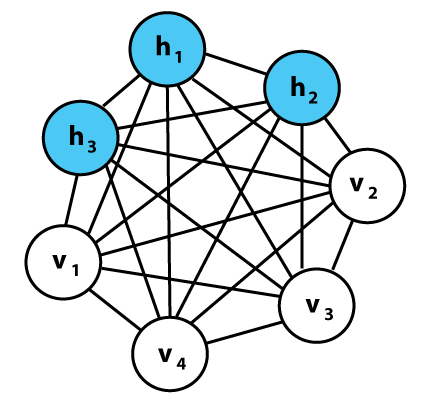
\includegraphics[width=0.3\linewidth]{figs/boltzmann}
	\caption{A non-restricted Boltzmann machine. The source is Wikipedia.}
	\label{fig:boltzmann}
\end{figure}

# \emph{Evolutionary methods} take a population of classifiers through many generations.
In each generation, new classifiers (offspring) are produced from the previous generation.
The best classifiers are subject to 
(1) replication, 
(2) crossover and 
(3) mutation to produce offspring.
The classifiers may be encoded as 2-bit chromosomes of length $L$.
The bits represent some property of the classifier.


# Genetic programming is the process of modifying formulas such as
\begin{equation*}
	\left[ (- x_1) + x_2 \right] / \left[ ( \ln x_3) - x_2 \right]
\end{equation*}
by evolutionary methods, mutating variables and operators and performing crossovers.
\end{easylist}


\subsection{Nonmetric methods}
\begin{easylist}[itemize]
\ListProperties(Space=\listSpace, Space*=\listSpace, Numbers1=l, FinalMark1={)})
# A \emph{decision tree} typically splits the feature space along the axes if the data is numeric, and works well for non-metric (categorical, or nominal) data as well.
To implement a decision tree, one must consider
## The number of splits made per node (typically 2, since a higher branching factor $B$ may be reduced to $B=2$ anyway).
## How to choose an attribute to split on -- often solved using \emph{information gain}.
## When a node should be declared a leaf node.
## How to handle missing data.

# To decide which attribute to split on, an \emph{impurity function} is defined for a node $N$ consisting of training samples from various categories $\omega_1, \dots, \omega_C$.
The impurity function should be 0 when all samples in node $N$ are from the same category $\omega_j$, and peak when the samples are uniformly drawn from the $C$ categories.

Two examples of impurity functions include the \emph{entropy impurity} and the \emph{Gini impurity}, which are respectively defined as
\begin{equation*}
	i(N) = - \sum_{j=1}^{C} P(\omega_j) \ln P(\omega_j) 
	\qquad
	i(N) =  \sum_{j=1}^{C} P(\omega_j) \sum_{k\neq j} P(\omega_k)
	= \sum_{j=1}^{C} P(\omega_j) \left[ 1 - P(\omega_j) \right].
\end{equation*}

A split is chosen so that it maximizes the decrease in impurity, i.e.
\begin{equation*}
	\Delta i(N) = i(N) - \left[ P_L \, i(N_L) + (1 - P_L) \, i(N_R)\right].
\end{equation*}
The equation says that the change in impurity equals the original impurity at node $N$ minus the weighted average of the impurity of the left and right child node.

# Other considerations in decision trees include:
## Pruning -- simplifying the tree after training (bypassing the horizon effect).
## Penalizing complexity -- regularization of the tree structure.
## Missing attributes -- for instance using (1) surrogate splits or (2) sending a training sample down every path and then performing a weighted average.

# Four \emph{string problems} in pattern classification are:
## \textbf{Matching}: naive matching is slow, the \emph{Boyer-Moore string matching algorithm} is much more efficient.
It operates by increasing the shift $s$ of $\vect{x}$ using two heuristics in parallel: the \emph{bad-character heuristic} and the \emph{good-suffix} heuristic.
## \textbf{Edit distance}: a way to compare the ``distance'' between strings by counting the number of insertions, deletions and substitutions required to transform $\vect{x}$ to $\vect{y}$.
If all costs are equal, then $D(\vect{x}, \vect{y})$ is a metric.
A dynamic programing algorithm is used to compute edit distance.
## \textbf{Matching with errors} is the same as matching, but using for instance the edit distance to find approximate matches. 
The problem is to find a shift $s$ that minimizes the edit distance.
## \textbf{Matching with the ``don't care''-symbol} $\emptyset$: same as matching, but the $\emptyset$-symbol matches any character in the alphabet $\mathcal{A}$.

# A grammar $G = (\mathcal{A}, \mathcal{I}, \mathcal{S}, \mathcal{P})$ consists of symbols $\mathcal{A}$, variables $\mathcal{I}$, a root symbol $\mathcal{S}$ and productions $\mathcal{P}$.
Concrete examples include English sentences and pronunciation of numbers.
There are several types of grammars, and they constitute a hierarchy
\begin{equation*}
	\text{Type} \, 3 \subset \text{Type} \, 2 \subset \text{Type} \, 1 \subset \text{Type} \, 0. 
\end{equation*}
The types are respectively called regular, context free, context sensitive and free.
## A central question is whether a string $\vect{x}$ is in the language $\mathcal{L}$ generated by the grammar $G$, i.e. whether $\vect{x} \in \mathcal{L}(G)$. This can be answered using bottom-up parsing, which employs the product rules $\mathcal{P}$ backwards.
\end{easylist}























\subsection{Algorithm-independent machine learning}
\begin{easylist}[itemize]
\ListProperties(Space=\listSpace, Space*=\listSpace, Numbers1=l, FinalMark1={)})
# The \emph{no free lunch theorem} states that using the off-training set error, and assuming equally likely target functions $F(\vect{x})$, no algorithm is universally superior.
Any statement about algorithms is a statement about the target function $F(\vect{x})$.

# The \emph{ugly duckling theorem} states that no feature representation is universally superior. 
If pattern similarity is based on the number of possible shared predicates ($f_1$ OR $f_2$, etc) then any two patterns are equally similar.
The best feature representation consequently depends on the target function $F(\vect{x})$.

# The \emph{minimum description length} is a version of Occam's razor.
In this framework, the best hypothesis $h$ (model) is the one compressing the data the most, i.e. the minimizer $h^*$ of
\begin{equation*}
	K(h, \D) = K(h) + K(\D \text{ using } h),
\end{equation*}
where $K(\cdot)$ is the Kolmogorov complexity (length of smallest computer program).

# The \emph{bias-variance trade-off} is exemplified by the equation
\begin{equation*}
	\E_\D \left[  \left( g(\vect{x}; \D) - F(\vect{x}) \right)^2  \right]
	=
	\underbrace{\E_\D \left[ g(\vect{x}; \D) - F(\vect{x})  \right]^2}_{\text{bias}^2}
	+
	\underbrace{\E_\D \left[  \left( g(\vect{x}; \D) - \E \left[ g(\vect{x}; \D) \right] \right)^2  \right]}_{\text{variance}},
\end{equation*}
and informally states that there is always a trade-off between bias and variance.
In the regression setting, the bias is the average error over many data sets, while the variance is the variability of the estimate over many data sets.
High variance typically implies many parameters (over-fitting), while high bias implies few parameters (under-fitting).

# The \emph{Jackknife} re-sampling method involves removing the $i$th data point from $\D = \{\vect{x}_1, \vect{x}_2, \dots, \vect{x}_n\}$ and computing a statistic.
This is done for every data point, and the final result is averaged.
From this the variance of the statistic may be assessed. 

# The \emph{bootstrap} method involves re-samling $n$ data points from $\D$ with replacement $B$ times.
The statistic is computed $B$ times, and is then averaged.
\begin{equation*}
	\hat{\theta}^{*(\cdot)} = \frac{1}{B} \sum_{b=1}^{B} \hat{\theta}^{*(b)}
	\qquad 
	\var_{\text{boot}} [ \hat{\theta} ]
	=
	\frac{1}{B} \sum_{b=1}^{B}
	\left( \hat{\theta}^{*(b)} - \hat{\theta}^{*(\cdot)} \right)^2 
\end{equation*}


# \emph{Bagging} consists of taking an average over model predictions.
\emph{Boosting} entails using the result of model $h^{n}$ to train model $h^{n+1}$.
Informally, the next model specializes on the data in $\D$ which the sequence of models so far has not performed well on.

## Adaptive Boosting (\emph{AdaBoost}) is a well known boosting algorithm.
It samples data $\vect{x}_i$ using probability weights $w_i$.
If a model $h^n$ does a poor job, the associated weights $w_i^{n+1}$ are increased exponentially. 
This causes exponential error decay on training data.

# \emph{Learning with queries} involves the model choosing the next data point to learn from.
It assumes the existence of an oracle which can give the correct answer to any input, but using this oracle might come with a cost.
Efficient learning involves choosing points where the classifier is uncertain, i.e. where $P(\omega_1 \mid \vect{x}) \approx P(\omega_2 \mid \vect{x})$.

# \emph{Maximum-likelihood model comparison} picks the maximum of
\begin{equation*}
	P(\D \mid h_i ) \simeq 
	\underbrace{P(\D \mid \hat{\vect{\theta}}, h_i)}_{\text{best-fit likelihood}}
	\underbrace{P(\hat{\vect{\theta}} \mid h_i) \Delta \vect{\theta}}_{\text{Occam factor}}
	= 
	P(\D \mid \hat{\vect{\theta}}, h_i)
	\frac{\Delta \vect{\theta}}{\Delta^0 \vect{\theta}},
\end{equation*}
where $\Delta \vect{\theta}$ is the volume of the possible parameter space given the data $\D$, and $\Delta^0 \vect{\theta}$ is the prior volume of the possible parameter before seeing data.
After some simplifications, this becomes a two step process: (1) compute maximum likelihood estimate $\hat{\vect{\theta}}$ from the data, then (2) compute the likelihood value given $\hat{\vect{\theta}}$.

# Mixture models can be used to combine classifiers using discriminant functions.
The final discriminant function is $g = \sum_{i=1}^{k} w_i g_i(\vect{x}, \vect{\theta}_i)$, and an underlying mixture model of the following form is assumed:
\begin{equation*}
	p(\vect{y} \mid \vect{x}, \vect{\Theta}^0)
	= \sum_{r=1}^{k}
	\underbrace{P(r \mid \vect{x}, \vect{\theta}_0^0 )}_{\text{prob. of model }r}
	p(\vect{y} \mid \vect{x}, \vect{\theta}_r^0 )
\end{equation*}





\end{easylist}



\subsection{Unsupervised learning and clustering}
\begin{easylist}[itemize]
	\ListProperties(Space=\listSpace, Space*=\listSpace, Numbers1=l, FinalMark1={)})
	# TODO :)
\end{easylist}




\clearpage
\section{Solutions to ``Pattern Classification''}

This section contains solutions to problems in ``Pattern Classification'' by Duda et al.
There are approximately 8 solved problems from each chapter.

\setcounter{subsection}{1}
\subsection{Bayesian Decision Theory}

\subsubsection*{Problem 2.6}
\begin{easylist}[enumerate]
\ListProperties(Space=\listSpace, Space*=\listSpace, Numbers1=l, FinalMark1={)})
# We want the probability of choosing action $\alpha_2$ to be smaller than, or equal to, $E_1$, given that the true state of nature is $\omega_1$.
Let's assume that $\mu_1 < \mu_2$ and that the decision threshold is $x^*$, so we decide $\alpha_2$ if $x > x^*$.
We then have
\begin{align*}
	P(\alpha_2  \mid  \omega_1) &\leq E_1 \\
	p(x > x^*  \mid  \omega_1) &\leq E_1 \\
	\left[1 - \int_{0}^{x^*} p(x  \mid  \omega_1)  \, dx \right] &\leq E_1
\end{align*}
We let $\Phi: \R \to \left[0, 1\right]$ denote the cumulative Gaussian distribution, and $\Phi^{-1}: \left[0, 1\right] \to \R$ it's inverse function.
Making use of $\Phi$ we write
\begin{align*}
1 - \Phi \left( \frac{x^* - \mu_1}{\sigma_1} \right) &\leq E_1 \\
x^* \geq \mu_1 + \sigma_1 \Phi^{-1} \left(1 - E_1 \right).
\end{align*}
If the desired error is close to zero, then $x^*$ goes to positive infinity.
If the desired error is close to one, then $x^*$ goes to negative infinity.

# The error rate for classifying $\omega_2$ as $\omega_1$ is
\begin{equation*}
	P(\alpha_1  \mid  \omega_2) = 	p(x \leq x^*  \mid  \omega_2) = \int_{0}^{x^*} p(x \mid  \omega_2) \, dx 
	= 
	\Phi \left(  \frac{x^* - \mu_2}{\sigma_2}  \right).
\end{equation*}
Making use of $x^*$ from the previous problem, we obtain
\begin{equation*}
 \Phi \left(  \frac{ \mu_1 + \sigma_1 \Phi^{-1} \left(1 - E_1 \right) - \mu_2}{\sigma_2}  \right) 
 =
\Phi \left(  \frac{\mu_1 - \mu_2}{\sigma_2} + \frac{\sigma_1}{\sigma_2}  \Phi^{-1} \left(1 - E_1 \right) \right).
\end{equation*}
# The overall error rate becomes
\begin{align*}
	P(\text{error}) &= P(\alpha_1, \omega_2) + P(\alpha_2, \omega_1) \\
	&= P(\alpha_1  \mid  \omega_2) P(\omega_2) + P(\alpha_2 \mid  \omega_1) P(\omega_1) \\
	&= \frac{1}{2} \left[  P(\alpha_1  \mid  \omega_2) +  P(\alpha_2 \mid  \omega_1) \right] \\
	&= \frac{1}{2} \left[ E_1 +  \Phi \left(  \frac{\mu_1 - \mu_2}{\sigma_2} + \frac{\sigma_1}{\sigma_2}  \Phi^{-1} \left(1 - E_1 \right) \right) \right].
\end{align*}
In the last equality we used the results from the previous subproblems.

# We substitute the given values into the equations, and obtain $x^* \approx 0.6449$. The total error rate is $P(\text{error}) \approx 0.2056$.
# The Bayes error rate, as a function of $x^*$, is given by
\begin{align*}
	P(\text{error}) = P(\alpha_2  \mid  \omega_1) P(\omega_1) + P(\alpha_1 \mid  \omega_2) P(\omega_2) \\
	= \frac{1}{2} \left[ p( x > x^* \mid  \omega_1)  + p( x < x^*  \mid  \omega_2) \right]   \\
	= \frac{1}{2} \left[ \left( 1 - \Phi \left( \frac{x^* - \mu_1}{\sigma_1}\right)\right) +  \Phi \left( \frac{x^* - \mu_2}{\sigma_2}\right)  \right]
\end{align*}
The Bayes error rate for this problem is depicted in Figure \ref{fig:duda_ch2_prob6}.

\begin{figure}[ht!]
\centering
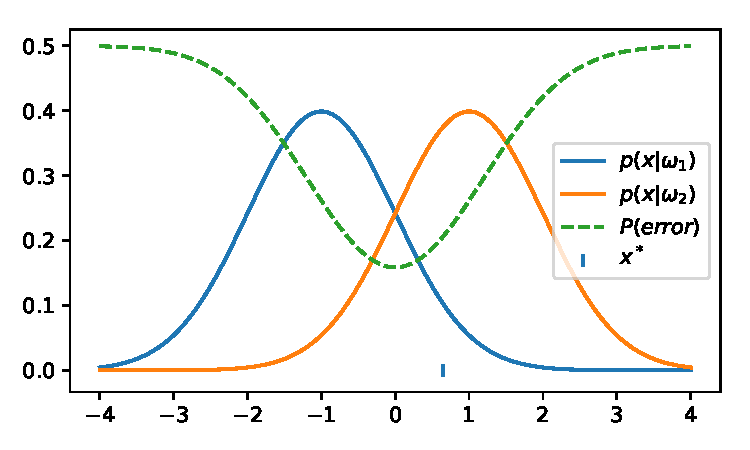
\includegraphics[width=0.5\linewidth]{figs/duda_ch2_prob6}
\caption{Graf accompanying problem 2.6.}
\label{fig:duda_ch2_prob6}
\end{figure}


\end{easylist}

\subsubsection*{Problem 2.12}
\begin{easylist}[enumerate]
\ListProperties(Space=\listSpace, Space*=\listSpace, Numbers1=l, FinalMark1={)})
# A useful observation is that the maximal value $P(\omega_{\text{max}}  \mid  \vect{x} )$ is greater than, or equal to, the average. Therefore we obtain
\begin{equation*}
	P(\omega_{\text{max}}  \mid  \vect{x} ) \geq \frac{1}{c} \sum_{i=1}^{c} P(\omega_i  \mid  \vect{x}) = \frac{1}{c},
\end{equation*}
where the last equality is due to probabilities summing to unity.
# The minimum error rate is achieved by choosing $\omega_{\text{max}}$, the most likely state of nature. 
The average probability of error over the data space is therefore the probability that $\omega_{\text{max}}$ is \emph{not} the true state of nature for a given $\vect{x}$, i.e.
\begin{equation*}
	P(\text{error}) = \E_x \left[ 1 - P(\omega_{\text{max}}  \mid  \vect{x} ) \right] = 1 - \int P(\omega_{\text{max}}  \mid  \vect{x} ) p(\vect{x}) \, d \vect{x}.
\end{equation*}

# We see that
\begin{equation*}
	P(\text{error}) = 1 - \int P(\omega_{\text{max}}  \mid  \vect{x} ) p(\vect{x}) \, d \vect{x} \leq 1 - \int \frac{1}{c} p(\vect{x}) \, d \vect{x} = 1 - \frac{1}{c} = \frac{c-1}{c},
\end{equation*}
where we have used the fact that $\int p(\vect{x}) \, d \vect{x} = 1$.


# A situation where $P(\text{error}) = (c-1)/c$ arises when $P(\omega_i) = 1/c$ for every $i$. Then the maximum value is equal to the average value, and the inequality in problem a) becomes an equality.
\end{easylist}


\subsubsection*{Problem 2.19}
\begin{easylist}[enumerate]
\ListProperties(Space=\listSpace, Space*=\listSpace, Numbers1=l, FinalMark1={)})
# The entropy is given by $\H\left[p(x)\right] = - \int p(x) \ln p(x) \, dx$.
The optimization problem gives the synthetic function (or Lagrange function)
\begin{align*}
	H_s = - \int p(x) \ln p(x) \, dx + \sum_{k=1} ^{q} \lambda_k \left( \int b_k(x) p(x) \, dx - a_k \right),
\end{align*}
and since a probability density function has $\int p(x) \, dx = 1$ we add an additional constraint for $k=0$ with $b_0(x) = 1$ and $a_k = 1$.
Collecting terms we obtain
\begin{align*}
H_s &= - \int p(x) \ln p(x) \, dx + \sum_{k=0} ^{q} \lambda_k  \int b_k(x) p(x) \, dx - \sum_{k=0} ^{q} \lambda_k a_k  \\
&= - \int p(x) 
\left[ \ln p(x) - \sum_{k=0} ^{q} \lambda_k b_k(x) \right] \, dx - \sum_{k=0} ^{q} \lambda_k a_k ,
\end{align*}
which is what we were asked to show.

# Differentiating the equation above with respect to $p(x)$ and equating it to zero we obtain
\begin{equation*}
	- \int \left(  1 \left[ \ln p(x) - \sum_{k=0} ^{q} \lambda_k b_k(x) \right] + p(x) \left[ \frac{1}{p(x)} \right] \right) \, dx = 0.
\end{equation*}
This integral is zero if the integrand is zero for every $x$, so we require that
\begin{equation*}
	 \ln p(x) - \sum_{k=0} ^{q} \lambda_k b_k(x) + 1 = 0,
\end{equation*}
and solving this equation for $p(x)$ gives the desired answer.
\end{easylist}

\subsubsection*{Problem 2.21}
We are asked to compute the entropy of the (1) Gaussian distribution, (2) triangle distribution and (3) uniform distribution. 
Every probability density function (pdf) has $\mu = 0$ and standard deviation $\sigma$, and we must write every pdf parameterized using $\sigma$.
\paragraph{Gaussian} We use the definition $\H\left[p(x)\right] = - \int p(x) \ln p(x) \, dx$ to compute  
\begin{equation*}
	\H\left[p(x)\right] = 
	- \int \frac{1}{\sqrt{2 \pi} \sigma} 
	\exp \left( - \frac{1}{2} \frac{x^2}{\sigma^2} \right) 
	\left[ \ln \left( \frac{1}{\sqrt{2 \pi} \sigma } \right) - \frac{1}{2} \frac{x^2}{\sigma^2} \right] \, dx.
\end{equation*}
Let us denote the constant by $K = \frac{1}{\sqrt{2 \pi} \sigma} $ to simplify notation. We obtain
\begin{align*}
	- \int & K
	\exp \left( - \frac{1}{2} \frac{x^2}{\sigma^2} \right) 
	\left[ \ln K - \frac{1}{2} \frac{x^2}{\sigma^2} \right] \, dx = \\
	- K \ln K \int & 
	\exp \left( - \frac{1}{2} \frac{x^2}{\sigma^2} \right) \, dx + K \int  \frac{1}{2} \frac{x^2}{\sigma^2} \exp \left( - \frac{1}{2} \frac{x^2}{\sigma^2} \right)  \, dx
\end{align*}
The first term evaluates to $-\ln K$, since it's the normal distribution with an additional factor $-\ln K$.
The second term is not as straightforward.
We change variables to $y = x / \left( \sqrt{2} \sigma \right)$, and write it as
\begin{equation*}
	K \int  y^2 \exp \left( - y^2 \right) \sqrt{2} \sigma \, dy,
\end{equation*}
and this integral is solved by using the following observation (from integration by parts):
\begin{equation*}
	\int 1 e^{-x^2} \, dx = \underbrace{\left. x e^{-x^2} \right|}_{0\text{ at } \pm \infty} - \int x (-2x) e^{-x^2} \, dx.
\end{equation*}
Using the above equation in reverse, we integrate as follows:
\begin{equation*}
	K \sqrt{2} \sigma \int  y^2 \exp \left( - y^2 \right)  \, dy = 	K \sqrt{2} \sigma \frac{1}{2}\int  \exp \left( - y^2 \right)  \, dy = K \sqrt{2} \sigma \frac{1}{2} \sqrt{\pi} = \frac{1}{2}
\end{equation*}
To recap, the first integral evaluated to $- \ln K$, and the second evaluated to $\frac{1}{2}$.
The entropy of the Gaussian is therefore $1/2 + \ln \sqrt{2 \pi } \sigma$.

\paragraph{Triangle}
The triangle distribution may be written in the form
\begin{equation*}
	f(x) = \begin{cases}
	h - \frac{hx}{b} &\quad \text{ if } \abs{x} < b\\
	0 &\quad \text{ if } \abs{x} \geq b,
	\end{cases}
\end{equation*}
where $h$ is the height and $b$ is the width to the left of, and to the right of, $x=0$.

Since the integral must evaluate to unity, we impose the constraint $hb = 1$ and obtain $f(x;b) = \frac{1}{b} \left( 1- \frac{x}{b}\right)$.
We wish to parameterize the triangle distribution using the standard deviation $\sigma$ instead of width $b$.
We can use $\var(X) = \E(X^2) - \E(X)^2$ to find the variance, since in this case $\E(X)^2 = \mu^2 = 0$ as a result of the function being centered on $x=0$.
Computing $\E(X^2)$ yields $b^2 / 6$, so $b^2 = 6 \sigma^2$.
The revised triangle distribution then becomes
\begin{equation*}
f(x; \sigma) = \begin{cases}
\frac{1}{\sqrt{6} \sigma} \left(1 - \frac{x}{\sqrt{6} \sigma}\right) &\quad \text{ if } \abs{x} < \sqrt{6} \sigma \\
0 &\quad \text{ if } \abs{x} \geq \sqrt{6} \sigma .
\end{cases}
\end{equation*}
We set $k = \frac{1}{\sqrt{6} \sigma}$ to ease notation.
Due to symmetry, we compute the entropy as 
\begin{equation*}
	\H\left[f(x; \sigma)\right] = - 2 \int_{0}^{\sqrt{6} \sigma} k \left(1 - kx\right) \ln \left( k \left(1 - k x \right) \right) \, dx.
\end{equation*}
Changing variables to $y = 1 - kx$ we obtain
\begin{align*}
& - 2 \int_{x=0}^{x=\sqrt{6} \sigma} k y  \left( \ln k + \ln y \right) \, dx = - 2 \int_{y = 1}^{y = 0} k y  \left( \ln k + \ln y \right) \left(\frac{1}{-k}\right) \, dy \\
& - 2 \int_{0}^{1} y \left( \ln k + \ln y \right) dy = - 2 \int_{0}^{1} y \ln k \, dy - 2 \int_{0}^{1} y  \ln y \, dy = -2 \left( \ln k - \frac{1}{4}\right),
\end{align*}
where the last integral can be evaluated using integration by parts.
The entropy of the triangle distribution turns out to be $1/2 + \ln \sqrt{6} \sigma$.

\paragraph{Uniform}
Using the same logic as with the triangle distribution, we first normalize a uniform distribution, and then parameterize by $\sigma$, to obtain
\begin{equation*}
u(x; \sigma) =
\left\{\!\begin{aligned}
\frac{1}{2b} &\quad \text{ if } \abs{x} < b \\
0 &\quad \text{ if } \abs{x} \geq b 
\end{aligned}\right\}
= 
\left\{\!\begin{aligned}
\frac{1}{2\sqrt{3}\sigma} &\quad \text{ if } \abs{x} <\sqrt{3}\sigma \\
0 &\quad \text{ if } \abs{x} \geq \sqrt{3}\sigma.
\end{aligned}\right.
\end{equation*}
Computing the entropy is more straightforward than in the case of the Gaussian and the triangle distribution.
We simply evaluate the integral as
\begin{equation*}
\H\left[p(x)\right] =2  \int_0^{\sqrt{3} \sigma} \frac{1}{2\sqrt{3}\sigma} \ln \frac{1}{2\sqrt{3}\sigma}  \, dx = \ln 2 \sqrt{3} \sigma.
\end{equation*}

Let's briefly compare the results of our computations as follows:
\begin{align*}
	H_\text{Gaussian}(\sigma) &= 1/2 + \ln \sqrt{2 \pi } \sigma = \frac{1}{2} + \ln \sqrt{2\pi}  + \ln \sigma \approx 1.4189 + \ln \sigma \\
	H_\text{Triangle}(\sigma) &= 1/2 + \ln \sqrt{6} \sigma = \frac{1}{2} + \ln \sqrt{6} + \ln \sigma \approx 1.3959 + \ln \sigma \\
	H_\text{Uniform}(\sigma) &= \ln 2 \sqrt{3} \sigma = 0 + \ln 2 \sqrt{3} + \ln \sigma \approx 1.2425 + \ln \sigma
\end{align*}
This verifies that out of the three distributions, the Gaussian has the maximal entropy.
This was expected, since the Gaussian maximizes the entropy over \emph{any} continuous probability density function having a prescribed mean and variance.



\subsubsection*{Problem 2.23}
\begin{easylist}[enumerate]
\ListProperties(Space=\listSpace, Space*=\listSpace, Numbers1=l, FinalMark1={)})
# To solve this problem, we need to find the inverse matrix, the determinant, and $\vect{w} = \vect{x} - \vect{\mu}$.
\begin{equation*}
	\vect{\Sigma}^{-1} = \frac{1}{21}\begin{pmatrix}
	1 & 0 & 0 \\
	0 & 5 & -2 \\
	0 & -2 & 5 \\
	\end{pmatrix}
	\quad
	\det \vect{\Sigma} = 21
	\quad
	\vect{w} = \vect{x} - \vect{\mu} = 
	\begin{pmatrix}
	-0.5 \\
	-2 \\
	-1
	\end{pmatrix}
\end{equation*}
The number of dimension $d$ is 3.
The solution is
\begin{equation*}
	p(\vect{x}) = \frac{1}{\left(2 \pi \right)^\frac{3}{2} 21^{\frac{1}{2}}} \exp \left( -\frac{1}{2} \vect{w}^T \vect{\Sigma}^{-1} \vect{w}\right)
	= \frac{1}{\left(2 \pi \right)^\frac{3}{2} 21^{\frac{1}{2}}} \exp \left( -\frac{1}{2} \frac{1}{21} \frac{69}{4}\right).
\end{equation*}
# The eigenvalues of $\vect{\Sigma}$ are $\lambda_1 = 3$, $\lambda_1 = 7$ and $\lambda_1 = 21$.
The corresponding eigenvectors are
$\vect{v}_1 = (0, 1, -1)^T / \sqrt{2}$, 
$\vect{v}_2 = (0, 1, 1)^T / \sqrt{2}$ and 
$\vect{v}_3 = (1, 0, 0)^T$.
The whitening transformation is therefore given by
\begin{equation*}
	\vect{A}_w = \vect{\Phi} \vect{\Lambda}^{-1/2} = 
	\frac{1}{\sqrt{2}}
	\begin{pmatrix}
	0 & 0 & \sqrt{2} \\
	1 & 1 & 0 \\
	-1 & 1 & 0 \\
	\end{pmatrix}
	\begin{pmatrix}
	-\sqrt{3} & 0 & 0 \\
	0 & -\sqrt{7} & 0 \\
	0 & 0 & -\sqrt{21} 
	\end{pmatrix}.
\end{equation*}
The rest of the numerical computations are skipped.
# Skipped.
# Skipped.
# We are going to examine if the p.d.f is unchanged when vectors are transformed with $\vect{T}^T \vect{x}$ and matrices with $\vect{T}^T \vect{\Sigma} \vect{T}$.
Let's consider the term $\left(\vect{x} - \vect{\mu}\right)^T \vect{\Sigma}^{-1} \left(\vect{x} - \vect{\mu}\right)$ in the exponent first.
Substituting $\vect{x} \mapsto \vect{T}^T \vect{x}$,
$\vect{\mu} \mapsto \vect{T}^T \vect{\mu}$ and
$\vect{\Sigma} \mapsto \vect{T}^T \vect{\Sigma} \vect{T}$, we observe that
\begin{gather*}
	\left(\vect{T}^T\vect{x} - \vect{T}^T\vect{\mu}\right)^T
	 \left( \vect{\vect{T}^T\Sigma}\vect{T}  \right)^{-1}
	 \left(\vect{T}^T\vect{x} - \vect{T}^T\vect{\mu}\right) \\
	\left(\vect{T}^T\left(\vect{x} - \vect{\mu}\right)\right)^T
	 \left( \vect{\vect{T}^T\Sigma}\vect{T}  \right)^{-1}
	 \vect{T}^T\left(\vect{x} - \vect{\mu}\right) \\
	 \left(\vect{x} - \vect{\mu}\right)^T \vect{T}
	 \left( \vect{T}^T \vect{\Sigma}\vect{T}  \right)^{-1}
	 \vect{T}^T\left(\vect{x} - \vect{\mu}\right) \\
	 \left(\vect{x} - \vect{\mu}\right)^T \vect{T}
	 \vect{T}^{-1} \vect{\Sigma}^{-1}\vect{T}^{-T}
	 \vect{T}^T\left(\vect{x} - \vect{\mu}\right) \\
	 \left(\vect{x} - \vect{\mu}\right)^T 
	  \vect{\Sigma}^{-1}
	 \left(\vect{x} - \vect{\mu}\right),
\end{gather*}
where we have used $(\vect{A}\vect{B})^T = \vect{B}^T \vect{A}^T$ and $(\vect{A}\vect{B})^{-1} = \vect{B}^{-1} \vect{A}^{-1}$, which are basic facts from linear algebra.
The density remains proportional when applying a linear transformation, but not unscaled, since the proportionality term $\abs{\vect{\Sigma}}^{1/2}$ becomes $\abs{\vect{T}^T \vect{\Sigma} \vect{T}}^{1/2} = \abs{\vect{T}^T}^{1/2}  \abs{\vect{\Sigma} }^{1/2}  \abs{ \vect{T}}^{1/2} = \abs{\vect{T}} \abs{\vect{\Sigma} }^{1/2}$.

# Here we use the eigendecomposition of a symmetric matrix.
We assume that $\vect{\Sigma}$ is positive definite such that every eigenvalue is positive. 
We write $\vect{\Sigma} = \vect{\Phi} \vect{\Lambda} \vect{\Phi}^T$ and apply the whitening transformation.
\begin{equation*}
	\vect{\vect{A}_w}^T \vect{\Sigma} \vect{\vect{A}_w} = 
	\vect{\vect{A}_w}^T \vect{\Phi} \vect{\Lambda} \vect{\Phi}^T \vect{\vect{A}_w}  = 
	\left( \vect{\Phi} \vect{\Lambda}^{-1/2} \right)^T \vect{\Phi} \vect{\Lambda} \vect{\Phi}^T \left( \vect{\Phi} \vect{\Lambda}^{-1/2} \right)
\end{equation*}
The matrix $\vect{\Phi}$ is orthogonal, so it's transpose is the inverse.
Using this fact and proceeding, we obtain
\begin{equation*}
\left( \vect{\Phi} \vect{\Lambda}^{-1/2} \right)^T \vect{\Phi} \vect{\Lambda} \vect{\Phi}^T \left( \vect{\Phi} \vect{\Lambda}^{1/2} \right) = \left( \vect{\Lambda}^{-1/2} \right)^T \vect{\Lambda} \vect{\Lambda}^{-1/2} = \vect{\Lambda}^{-1/2} \vect{\Lambda} \vect{\Lambda}^{-1/2} = \vect{I},
\end{equation*}
so the covariance is proportional to the identity matrix, as we were tasked to show.
The normalization constant becomes $1$ , since the proportionality term becomes $\abs{\vect{T}} \abs{\vect{\Sigma} }^{1/2}$ under the transformation, and 
\begin{equation*}
	\abs{\vect{T}} \abs{\vect{\Sigma} }^{1/2} = \abs{\vect{\Phi} \vect{\Lambda}^{-1/2}} \abs{\vect{\Sigma} }^{1/2} = \abs{\vect{\Phi} \vect{\Lambda}^{-1/2}} \abs{\vect{\Phi} \vect{\Lambda} \vect{\Phi}^T }^{1/2} = \abs{\vect{I}} = 1.
\end{equation*}
\end{easylist}

\subsubsection*{Problem 2.28}
\begin{easylist}[enumerate]
\ListProperties(Space=\listSpace, Space*=\listSpace, Numbers1=l, FinalMark1={)})
# We prove that if 
\begin{equation*}
	p(x_i - \mu_i, x_j - \mu_j) = p(x_i - \mu_i) p(x_j - \mu_j),
\end{equation*}
then
\begin{equation*}
\sigma_{ij} = \E \left[ (x_i - \mu_i) (x_j - \mu_j)\right] = 0.
\end{equation*}
With words: we prove that statistical independence implies zero covariance.
\begin{gather*}
	 \E \left[ (x_i - \mu_i) (x_j - \mu_j)\right] = \\
	 \iint p(x_i - \mu_i, x_j - \mu_j) (x_i - \mu_i) (x_j - \mu_j) \, dx_j dx_i = \\
	 \iint  p(x_i - \mu_i) p(x_j - \mu_j) (x_i - \mu_i) (x_j - \mu_j) \, dx_j dx_i \\
	 \int p(x_i - \mu_i) (x_i - \mu_i) \left( 
	 \int p(x_j - \mu_j) (x_j - \mu_j) \, dx_j
	   \right) \, dx_i
\end{gather*}
If the term in the parenthesis is identically zero, then $\sigma_{ij} = 0$.
This is indeed true, since the integral is
\begin{equation*}
	\int p(x_j - \mu_j) (x_j - \mu_j) \, dx_j = \E \left[ (x_j - \mu_j)\right]
	= \E \left[x_j\right] -  \E \left[\mu_j\right] = \mu_j - \mu_j = 0.
\end{equation*}
# We wish to prove the converse of a) in the Gaussian case.
To achieve this, we must show that
$\sigma_{ij} = 0$ when 
\begin{equation*}
	p(x_i - \mu_i, x_j - \mu_j) = p(x_i - \mu_i) p(x_j - \mu_j).
\end{equation*}

Let's simplify the notation to $x$ and $y$ instead of $x_i$ and $x_j$.
If $\sigma_{xy} = 0$, then the covariance matrix is a diagonal matrix $\vect{D} = \operatorname{diag}(\sigma_x^2, \sigma_y^2)$.
We write the probability $p(x_i - \mu_i, x_j - \mu_j)$ as $p(x,y)$, where the means $\mu_x$ and $\mu_y$ are both zero.
We write
\begin{gather*}
	p(x, y) = 
	\frac{1}{(2\pi)^{2/2} \sigma_x \sigma_y} \exp \left( - \frac{1}{2} \vect{x}^T \vect{D}^{-1} \vect{x} \right) = 
	\frac{1}{(2\pi)^{2/2} \sigma_x \sigma_y} \exp \left( - \frac{1}{2} \left( x^2 / \sigma_x^2 + y^2 / \sigma_y^2 \right) \right)  \\
	=  \frac{1}{(2\pi)^{1/2} \sigma_x} \exp \left( - \frac{1}{2} \left( x^2 / \sigma_x^2 \right) \right) 
	\frac{1}{(2\pi)^{1/2} \sigma_y} \exp \left( - \frac{1}{2} \left( y^2 / \sigma_y^2 \right) \right)
	= p(x) p(y).
\end{gather*}
This demonstrates that when $\sigma_{xy} = 0$, the covariance matrix is diagonal, and the Gaussian factors into products and we have statistical independence.

# This problem asks us to find a counterexample of the above, i.e. an example showing that $\sigma_{xy} \nRightarrow p(x, y) = p(x) p(y)$.
The probability density function
\begin{equation*}
	p(x, y) = K \frac{1}{1 + x^2 + y^2}, \quad K^{-1} = \iint_{\R} \frac{1}{1 + x^2 + y^2} \, dx dy
\end{equation*}
achieves this.
The covariance is zero, since 
\begin{equation*}
	\sigma_{xy} = \E \left[ (x - 0) (y - 0)\right] = \iint_{\R} \frac{x y}{1 + x^2 + y^2} \, dx dy = \iint_{\R} I(x, y) \, dx dy
\end{equation*}
is zero because the integrand $I(x, y)$ is an odd function.

On the other hand, $p(x, y)$ does \emph{not} factor into $p(x) p(y)$.
We have proved that $\sigma_{xy} \nRightarrow p(x, y) = p(x) p(y)$ by finding a counterexample.
\end{easylist}
\subsubsection*{Problem 2.31}
\begin{easylist}[enumerate]
\ListProperties(Space=\listSpace, Space*=\listSpace, Numbers1=l, FinalMark1={)})
# We'll assume that $\mu_1 < \mu_2$.
Since $\sigma_1 = \sigma_2 = \sigma$, the minimum probability of error is achieved by setting the decision threshold to $x^* = (\mu_1 + \mu_2)/2$.
When following the derivation below, it is illuminating to draw the real line and two Gaussians.
The probability of error is
\begin{align*}
	P_e &= P(x \in R_2, \omega_1) + P(x \in R_1, \omega_2) \\
	&= 
	P(x \in R_2  \mid  \omega_1) P(\omega_1)  + P(x \in R_1  \mid  \omega_2) P(\omega_2) \\&= 
	\int_{R_2} p(x  \mid  \omega_1) P(\omega_1) \, dx + \int_{R_1} p(x  \mid  \omega_2) P(\omega_2) \, dx
	 \\
	 &= \frac{1}{2}\left( \int_{x^*}^{\infty} p(x  \mid  \omega_1) \, dx + 
	 \int_{0}^{x^*} p(x  \mid  \omega_2) \, dx \right) = \int_{x =(\mu_1 + \mu_2)/2 }^{\infty} p(x  \mid  \omega_1) \, dx \\
	 &=
	 \int_{x =(\mu_1 + \mu_2)/2 }^{\infty} \frac{1}{\sqrt{2 \pi } \sigma} \exp\left( - \frac{1}{2} \frac{(x - \mu_1)^2}{\sigma^2}\right) \, dx.
\end{align*}
Changing variables to $u = (x - \mu_1) / \sigma$ and using $dx = \sigma \, du$ yields
\begin{equation*}
	P_e = \int_{u=a}^{\infty} \frac{1}{\sqrt{2 \pi }} \exp\left( -u^2 /\sigma^2 \right) \, du,
\end{equation*}
where $a = (x - \mu_1 )/\sigma = ((\mu_1 + \mu_2)/2 - \mu_1 )/\sigma =  (\mu_2 - \mu_1) / 2 \sigma$, as required.

# Using the inequality stated in the problem, it remains to show that
\begin{equation*}
	\lim_{a \to \infty} f(a) = \lim_{a \to \infty} \frac{1}{\sqrt{2 \pi} a} \exp\left( -a^2 /\sigma^2 \right) = 0.
\end{equation*}
This holds if the derivative is negative as $a \to \infty$, since then the function decreases as $a \to \infty$. The derivative of $f(a)$ is
\begin{equation*}
	f'(x) = -\exp\left( -a^2 / 2\right) \left( 1 - \frac{1}{a^2}\right),
\end{equation*}
which is negative as long as $\abs{a} \geq 1$.
Alternatively, we can simple note that both factors in $f(a)$ go to zero as $a \to \infty$.
\end{easylist}

\subsubsection*{Problem 2.43}
\begin{easylist}[enumerate]
	\ListProperties(Space=\listSpace, Space*=\listSpace, Numbers1=l, FinalMark1={)})
	# $p_{ij}$ is the probability that the $i$'th entry in the vector $\vect{x}$ equals $1$, given a state of nature $\omega_j$.
	# We decide $\omega_j$ if $P(\omega_j  \mid  \vect{x})$ is greater than $P(\omega_k  \mid  \vect{x})$ for every $k \neq j$.
	\begin{equation*}
	P(\omega_j  \mid  \vect{x}) \propto p(  \vect{x}  \mid  \omega_j) P(\omega_j)
	\end{equation*}
	We use the equation $p(  \vect{x}  \mid  \omega_j) = \prod_{i = 1}^{d} p(  x_i \mid  \omega_j)$, which follows from the fact that the entries are statistically independent.
	Furthermore, we see that
	\begin{equation*}
	p(  x_i \mid  \omega_j) = 
	\left\{\!\begin{aligned}
	p_{ij} &\quad \text{ if } x_i = 1 \\
	1 - p_{ij} &\quad \text{ if } x_i = 0 
	\end{aligned}\right\} = 
	p_{ij}^{x_i} \left( 1 - p_{ij}\right)^{ 1 - x_i}.
	\end{equation*}
	Now we take logarithms and  obtain
	\begin{align*}
	& \ln \left( \prod_{i = 1}^{d} p(  x_i \mid  \omega_j) P(\omega_j) \right) =
	\sum_{i = 1}^{d} \ln p(  x_i \mid  \omega_j)  + \ln P(\omega_j) \\
	& = \sum_{i = 1}^{d} \ln p_{ij}^{x_i} \left( 1 - p_{ij}\right)^{ 1 - x_i}  + \ln P(\omega_j) \\
	&
	= \sum_{i = 1}^{d} x_i \ln p_{ij} + (1 - x_i) \ln ( 1 - p_{ij})  + \ln P(\omega_j),
	\end{align*}
	which is easily arranged to correspond with the expression in the problem statement. 
	In summary we choose the class $\omega_j$ if the probability of that class given the data point exceeds the probability of every other class.
\end{easylist}



\clearpage
\subsection{Maximum-likelihood and Bayesian parameter estimation}

\subsubsection*{Problem 3.2}
\begin{easylist}[enumerate]
\ListProperties(Space=\listSpace, Space*=\listSpace, Numbers1=l, FinalMark1={)})
# The maximum likelihood estimate for $\theta$ is $\max_\theta p(\D  \mid  \theta) = \max_\theta \prod_{i=1}^{n} p(x_i  \mid  \theta)$.
The probability of a single sample $p(x_i  \mid  \theta)$ is given by the expression
\begin{equation*}
	p(x_i  \mid  \theta) = 
	\begin{dcases*}
	1/\theta & if $0 \leq x_i \leq \theta$ \\
	0 & if $ x_i > \theta$.
	\end{dcases*}
\end{equation*}
Clearly the product $\prod_{i=1}^{n} p(x_i  \mid  \theta)$ is zero if any $x_i$ is larger than $\theta$.
Therefore $\theta$ must be larger than, or equal to, $\max_k x_k$ for the likelihood to be non-zero.

On the other hand, the product equals $1 /\theta^n$, and taking logarithms we obtain $-n \ln \theta$.
This function is maximized when $\theta$ is as small as possible.

The conclusion is that $\theta$ must be greater than or equal to $\max_k x_k$ to avoid the likelihood being zero, and also as small as possible to maximize the likelihood.
Therefore the maximum likelihood is given by $\hat{\theta} = \max_k x_k = \max \D$.

# Skipping this plot. 
The explanation of why the other data points are not needed is given in part a) of the problem.
\end{easylist}

\subsubsection*{Problem 3.4}
The maximum likelihood estimate is 
\begin{equation*}
	p( \D  \mid  \vect{\theta}) = \prod_{k = 1}^{n} p( \vect{x}  \mid  \vect{\theta}) = \prod_{k = 1}^{n} \prod_{i=1}^{d}
	\theta_{i}^{x_{ik}} \left( 1 - \theta_i \right)^{\left(  1 - x_{ik} \right)}.
\end{equation*}
 The log likelihood $\ell(\vect{\theta})$ is $ \ln p( \D  \mid  \vect{\theta}) $, which is given by the expression
 \begin{equation*}
 	\ell(\vect{\theta}) = \sum_{k = 1}^{n} \sum_{i=1}^{d}
 	x_{ik} \ln \theta_i + (1 - x_{ik}) \ln \left( 1 - \theta_i\right).
 \end{equation*}
Differentiating $\ell(\vect{\theta})$ with respect to $\theta_i$, every term in the sum $\sum_{i=1}^{d}$ vanishes except the $i$'th.
We perform the differentiation and equate the result to zero, which yields
\begin{equation*}
	\frac{d \ell(\vect{\theta})}{\theta_i} = \sum_{k=1}^{n} \left[ \frac{x_{ik}}{\theta_i} + \frac{x_{ik} - 1}{1 - \theta_i} \right] =
	 \sum_{k=1}^{n} \left[ x_{ik} - \theta_i \right] = 0.
\end{equation*}
Solving this for $\theta_i$ gives us $\theta_i = n^{-1} \sum_{k=1}^{n} x_{ik}$, or in vector notation, $\vect{\theta} = n^{-1} \sum_{k=1}^{n} \vect{x}_k$.
This is what the problem asked us to show.


\subsubsection*{Problem 3.13}
\begin{easylist}[enumerate]
\ListProperties(Space=\listSpace, Space*=\listSpace, Numbers1=l, FinalMark1={)})
# Familiarity with summation notation helps when solving this problem.
The matrix-vector product $\vect{A}\vect{a}$ may be written as $\sum_j A_{ij} a_j$.
The sum is typically taken over repeated indices, but we will explicitly typeset the summation index.

Let's write the outer product as $\vect{a}\vect{b}^T = a_i \oplus b_j$, the trace as $\operatorname{tr}(\vect{A}) = \sum_i A_{ii}$ and
\begin{equation*}
	\operatorname{tr}(\vect{a}\vect{b}^T) = \sum_{i = j} a_i \oplus b_j = \sum_{i} a_i b_i.
\end{equation*}
We note that the effect of $\sum_{i = j}$ on a summand is to replace $i$ by $j$, or vice versa.

In summation notation, $\vect{a}^T \vect{A} \vect{a} = \sum_i \sum_j A_{ij} a_j a_i$.
Using the definitions above, and recalling that $\vect{A} \vect{a}$ is just a vector with value $\sum_j A_{ij} a_j$ in the $i$'th index, we see that
\begin{equation*}
	\operatorname{tr}( \vect{A} \vect{a} \vect{a}^T) = \sum_{i=k}  \left( \sum_j A_{ij} a_j \right) \oplus a_k = \sum_i \sum_j A_{ij} a_j a_i.
\end{equation*}

# The likelihood is given by the expression
\begin{align*}
	p(\D  \mid  \theta) &= \prod_{k=1}^{n} \frac{\abs{\vect{\Sigma}^{-1}}^{1/2}}{\left(2 \pi \right)^{d/2}} \exp \left( -\frac{1}{2} \left( \vect{x}_k - \vect{\mu} \right)^T  \vect{\Sigma}^{-1}  \left( \vect{x}_k - \vect{\mu} \right)\right) \\
	&=  \frac{\abs{\vect{\Sigma}^{-1}}^{n/2}}{\left(2 \pi \right)^{nd/2}} \exp \left( -\frac{1}{2}  \sum_{k=1}^{n} \left( \vect{x}_k - \vect{\mu} \right)^T  \vect{\Sigma}^{-1}  \left( \vect{x}_k - \vect{\mu} \right)\right).
\end{align*}
Applying $ \vect{a}^T \vect{A} \vect{a} = \operatorname{tr}( \vect{A} \vect{a} \vect{a}^T)$ from problem a) yields
\begin{equation*}
p(\D  \mid  \theta) = \frac{\abs{\vect{\Sigma}^{-1}}^{n/2}}{\left(2 \pi \right)^{nd/2}} \exp \left( -\frac{1}{2}  \sum_{k=1}^{n} 
\operatorname{tr} \left( \vect{\Sigma}^{-1} \left( \vect{x}_k - \vect{\mu} \right) \left( \vect{x}_k - \vect{\mu} \right)^T \right)
\right),
\end{equation*}
and by using $\operatorname{tr}\left(\vect{A} + \vect{B}\right) = \operatorname{tr}\left(\vect{A}\right) + \operatorname{tr}\left( \vect{B}\right)$ on the exponent we complete the problem.

# To solve this problem, we make use of two proofs from linear algebra.

\begin{easylist}
\ListProperties(Space=\listSpace, Space*=\listSpace, Numbers1=l, Numbers2=r, FinalMark1={)})
## The determinant is the product of the eigenvalues, i.e. $\det \vect{A} = \prod_{i=1}^{d} \lambda_i$.
This can be proved by taking the determinant of the eigenvalue decomposition of $\vect{A}$, i.e. $\vect{A}  = \vect{Q}  \vect{\Lambda} \vect{Q}^T$, since the determinant of an orthogonal matrix is unity and $\vect{\Lambda}$ has eigenvalues on the diagonal, the result is that $\det \vect{A} = \abs{\vect{A}} = \prod_{i=1}^{d} \lambda_i$.
## The trace is the sum of the eigenvalues, i.e. $\operatorname{tr} \vect{A} =\sum_{i=1}^{d} \lambda_i$. The proof for this involves characteristic polynomials, but is not sketched here.
\end{easylist}

The term involving $\vect{\Sigma}^{-1}$ is transformed in the following way: if $\vect{A} = \vect{\Sigma}^{-1} \hat{\vect{\Sigma}}$, then $\abs{\vect{A}} = \abs{\vect{\Sigma}^{-1}} | \hat{\vect{\Sigma}} |$. 
We then write the determinant of the inverse matrix as
\begin{equation*}
	\abs{\vect{\Sigma}^{-1}} = \frac{\abs{\vect{A}}}{| \hat{\vect{\Sigma}} |} = \frac{\prod_{i=1}^{d} \lambda_i}{| \hat{\vect{\Sigma}} |}.
\end{equation*}

To transform the exponent, we write
\begin{equation*}
	 \operatorname{tr} \left( \sum_{k=1}^{n}  \vect{\Sigma}^{-1} \left( \vect{x}_k - \vect{\mu} \right) \left( \vect{x}_k - \vect{\mu} \right)^T \right)
	 =
	 \operatorname{tr} \left( \vect{\Sigma}^{-1} n \hat{\vect{\Sigma}}  \right)
	 =
	 n  \operatorname{tr} \left( \vect{A} \right) = n \sum_{i=1}^{d} \lambda_i.
\end{equation*}
Substituting these transformation into the previous equation yields the required expression, which is
\begin{equation}
\label{eq:prob3_13}
	p(\D  \mid  \theta) = \frac{\left( \prod_{i=1}^{d} \lambda_i \right)^{n/2}}{\left(2 \pi \right)^{nd/2} \hat{\abs{\vect{\Sigma}}}^{n/2} } \exp \left( -\frac{n}{2} \sum_{i=1}^{d} \lambda_i \right).
\end{equation}

# Taking logarithms of Equation \eqref{eq:prob3_13} above gives us the log-likelihood function
\begin{equation*}
	\ln p(\D  \mid  \theta) = \frac{n}{2} \left[ \sum_{i=1}^{d} \ln \lambda_i - d \ln 2 \pi - \ln | \hat{\vect{\Sigma}} |  \right] - \frac{n}{2} \sum_{i=1}^{d} \lambda_i,
\end{equation*}
and differentiating it with respect to the eigenvalue $\lambda_j$ yields 
\begin{equation*}
	\frac{\partial \ln p(\D  \mid  \theta)}{\partial \lambda_j} = \frac{n}{2} \left(1 - \lambda_j^2 \right) = 0.
\end{equation*}
The Hessian matrix (second derivative) is a diagonal matrix with $-2\lambda_j$ on the $(j, j)$'th entry, so it is negative definite (i.e. $\vect{x}^T \vect{H} \vect{x} < 0$ for every $\vect{x} \neq 0$) when all $\lambda_j$'s are positive.
When the Hessian is negative definite, then the solution is a maximum.
Therefore we take $\lambda_j = 1$ as the solution for every $j$ (and not $\lambda_j = -1$, which is not a maximum point).

If every eigenvalues of $\vect{A}$ is $1$, then $\vect{A} = \vect{I}$.
Recall that $\vect{A} = \vect{\Sigma}^{-1} \hat{\vect{\Sigma}}$, so when we substitute the identity for $\vect{A}$ we obtain $\vect{\Sigma}^{-1} \hat{\vect{\Sigma}} = \vect{I}$.
The likelihood is maximized when we take $\hat{\vect{\Sigma}}$ to be $ n^{-1} \sum_{k=1}^{n} \left( \vect{x}_k - \vect{\mu} \right) \left( \vect{x}_k - \vect{\mu} \right)^T$, and the proof is complete.
\end{easylist}

\subsubsection*{Problem 3.15}
\begin{easylist}[enumerate]
\ListProperties(Space=\listSpace, Space*=\listSpace, Numbers1=l, FinalMark1={)})
# Starting with Equation (31) from the book, we get rid of $\sigma_n^2$ by substituting the expression given in Equation (32) to obtain
\begin{equation*}
\mu_n =
\underbrace{ \left[ \frac{1}{\frac{n}{\sigma^2} + \frac{1}{\sigma_0^2}} \right]}_{\sigma^2_n}
\frac{n}{\sigma^2} \hat{\mu}_n + 
\underbrace{ \left[ \frac{1}{\frac{n}{\sigma^2} + \frac{1}{\sigma_0^2}} \right]}_{\sigma^2_n}
\frac{\mu_0}{\sigma_0^2}.
\end{equation*}
We cancel terms, use the dogmatism $n_0 = \sigma^2 / \sigma_0^2$, and realize that $\mu_0 = n_0^{-1} \sum_{k = -n_0 + 1}^{0} x_k$.
\begin{align*}
\mu_n &= \left[ \frac{1}{1 + \frac{\sigma^2}{n \sigma_0^2}}  \right]
\hat{\mu}_n + 
\left[ \frac{1}{1 + \frac{n \sigma_0^2}{\sigma^2}} \right] \mu_0 \\
&= \left[ \frac{1}{1 + \frac{n_0}{n}}  \right]
\frac{1}{n} \sum_{k = 1}^{n} x_k
+ 
\left[ \frac{1}{1 + \frac{n}{n_0}} \right]
 \frac{1}{n_0} \sum_{k = -n_0 + 1}^{0} x_k
 \\
 &= \frac{1}{n + n_0} \sum_{k = 1}^{n} x_k + 
 \frac{1}{n + n_0} \sum_{k = -n_0 + 1}^{0} x_k = 
 \frac{1}{n + n_0} \sum_{k = -n_0 + 1}^{n} x_k.
\end{align*}

## One interpretation of $\mu_n$ is that it's a weighted average of the real samples and the fictitious samples, since
\begin{equation*}
	\mu_n = 
	\frac{n}{n + n_0} \left[ \frac{1}{n} \sum_{k = 0}^{n} n \right] 
	+
	\frac{n_0}{n + n_0} \left[ \frac{1}{n_0} \sum_{k = -n_0 + 1}^{0} x_k \right] = 
	\frac{1}{n + n_0} \sum_{k = -n_0 + 1}^{n} x_k.
\end{equation*}
An interpretation of $\sigma_n^2$ is more straightforward if we consider it's reciprocal, the \emph{precision} $\sigma_n^{-2}$.
The precision can be written as $\sigma_n^{-2} = n \sigma^{-2} + n_0 \sigma^{-2}$, so the number of fictitious samples provides an initial estimate for the precision, and as more real data points are added the precision is increased linearly.
	
\end{easylist}

\subsubsection*{Problem 3.16}
\begin{easylist}[enumerate]
	\ListProperties(Space=\listSpace, Space*=\listSpace, Numbers1=l, FinalMark1={)})
	# The trick is to multiply both terms by $\vect{I}$ at an opportune moment, expanding the identity and using $\left(\vect{A} \vect{B}\right)^{-1} = \vect{B}^{-1} \vect{A}^{-1}$. 
	We prove the theorem by writing
	\begin{align*}
	\left( \vect{A}^{-1} + \vect{B}^{-1}\right)^{-1} &=
		\left( \vect{A}^{-1} \vect{I} + \vect{I}\vect{B}^{-1}\right)^{-1} =
		\left( \vect{A}^{-1} \vect{B} \vect{B}^{-1} + \vect{A}^{-1} \vect{A}\vect{B}^{-1}\right)^{-1} \\
		&=  \left( \vect{A}^{-1} \left( \vect{B} + \vect{A} \right) \vect{B}^{-1} \right)^{-1} = 
		 \vect{B}\left( \vect{A} + \vect{B} \right)^{-1} \vect{A}.
	\end{align*}
	Replacing the second equality by $\vect{I} \vect{A}^{-1}  + \vect{B}^{-1} \vect{I} = \vect{B}^{-1} \vect{B}  \vect{A}^{-1} + \vect{B}^{-1} \vect{A} \vect{A}^{-1}$ would yield the second quality in the theorem as stated in the problem.
	
	# The matrices must be square, since we use $\vect{I} = \vect{A}^{-1} \vect{A}$ to prove the first equality, and $\vect{I} = \vect{A}^{-1} \vect{A}$ to prove the second. The same logic applies to $\vect{B}$.
	In other words, we require that $\vect{A}$ has a left-inverse and a right-inverse, and it must therefore be square.
	
	An alternative approach is to consider the second equality in the theorem directly.
	Some algebra reveals that this equality requires $\vect{A}$ to have a left and right inverse.
	It must therefore be square, against since no non-square matrix has a left-inverse and a right-inverse.
	
	# The staring point are the equations
	\begin{equation*}
		\vect{\Sigma}_n^{-1} = n \vect{\Sigma}^{-1} + \vect{\Sigma}_0^{-1}
		\quad \text{ and } \quad
		\vect{\Sigma}_n^{-1} \vect{\mu}_n 
		=n \vect{\Sigma}^{-1} \hat{\vect{\mu}}_n 
		+
		\vect{\Sigma}^{-1}_0 + \vect{\mu}_0,
	\end{equation*}
	and we wish to solve these equations with respect to $\vect{\Sigma}_n$ and $\vect{\mu}_n$. 
	In other words, we want the functional dependence to be 
	$\vect{\Sigma}_n = f \left( \hat{\vect{\mu}}_n, \vect{\mu}_0, \vect{\Sigma}, \vect{\Sigma}_0 \right)$
	and $\vect{\mu}_n = \left( \hat{\vect{\mu}}_n, \vect{\mu}_0, \vect{\Sigma}, \vect{\Sigma}_0 \right)$.
	
	We start with the covariance matrix. 
	To solve for $\vect{\Sigma}_n$, we write
	\begin{align*}
		\vect{\Sigma}_n = \left(\vect{\Sigma}_n^{-1}\right)^{-1} = \left(  n \vect{\Sigma}^{-1} + \vect{\Sigma}_0^{-1} \right)^{-1} = 
		\vect{\Sigma}_0 \left( \vect{\Sigma}_0 + \frac{1}{n}  \vect{\Sigma} \right)^{-1} \frac{1}{n} \vect{\Sigma},
	\end{align*}
	where the last equality comes from using 
	\begin{equation*}
		\left( \vect{A}^{-1} + \vect{B}^{-1}\right)^{-1} =
		\vect{B}^{-1} \left( \vect{B} + \vect{A} \right)^{-1} \vect{A}^{-1}.
	\end{equation*}
	
	To solve for the mean $\vect{\mu}_n$, we write
	\begin{align*}
		\vect{\mu}_n 
		&= \vect{\Sigma}_n n \vect{\Sigma}^{-1} \hat{\vect{\mu}}_n 
		+
		\vect{\Sigma}_n \vect{\Sigma}^{-1}_0  \vect{\mu}_0
		\\ &=
		\left[ \vect{\Sigma}_0 \left( \vect{\Sigma}_0 + \frac{1}{n}  \vect{\Sigma} \right)^{-1} \frac{1}{n} \vect{\Sigma} \right] n \vect{\Sigma}^{-1} \hat{\vect{\mu}}_n 
		+
		\left[  \frac{1}{n} \vect{\Sigma} \left(  \frac{1}{n}  \vect{\Sigma} + \vect{\Sigma}_0  \right)^{-1}  \vect{\Sigma}_0 \right] \vect{\Sigma}^{-1}_0  \vect{\mu}_0 \\
		& = 
		 \vect{\Sigma}_0 \left( \vect{\Sigma}_0 + \frac{1}{n}  \vect{\Sigma} \right)^{-1}  \hat{\vect{\mu}}_n 
		+
		 \frac{1}{n} \vect{\Sigma} \left( \vect{\Sigma}_0 + \frac{1}{n}  \vect{\Sigma}  \right)^{-1}   \vect{\mu}_0 
	\end{align*}
	Where we made use of both equalities given by the theorem in subproblem a).
\end{easylist}


\subsubsection*{Problem 3.24}
Our task is to find the maximum likelihood estimate of $\theta$ in the Rayleigh distribution, which is given by the expression
\begin{equation*}
	p (x  \mid  \theta) = 
	\begin{dcases*}
	2 \theta x \exp \left( -\theta x^2 \right) & if $x \geq 0$ \\
	0 & otherwise.
	\end{dcases*}
\end{equation*}
The log-likelihood function is given by
\begin{equation*}
	\ell(\theta)= \ln \left( p (\D  \mid  \theta) \right) 
	= 
	\sum_{k=1}^{n} \ln \left( 2 \theta x \exp \left( -\theta x^2 \right) \right)
	= 
	\sum_{k=1}^{n} - \theta x_i^2 + \ln 2 \theta x_i.
\end{equation*}
Differentiating the log-likelihood with respect to $\theta$ and equating it to zero yields
\begin{equation*}
	\ell'(\theta) =
	\sum_{k=1}^{n} \left(-  x_i^2 + \frac{2 x_i}{2 \theta x_i}\right)
	=
	\sum_{k=1}^{n} \left(-  x_i^2 + \frac{1}{\theta}\right)
	=
	\frac{n}{\theta} - \sum_{k=1}^{n}  x_i^2 
	= 0,
\end{equation*}
and solving this equation for $\theta$ reveals the desired answer.



\subsubsection*{Problem 3.32}
\begin{easylist}[enumerate]
\ListProperties(Space=\listSpace, Space*=\listSpace, Numbers1=l, FinalMark1={)})
# A simple $\Theta(n^2)$ algorithm is given by
\begin{lstlisting}
    f = 0
    for i=0 to n-1 do:
      f = f + a[i] * x**i
    end
\end{lstlisting}
Assuming that the computation of $x^i$ requires $i-1$ flops, the complexity for iteration $i$ is $\Theta(i)$, and the full complexity becomes $1 + 2 + 3 + \dots + (n-1) = \Theta(n^2)$.

# The waste in the algorithm from subproblem a) above stems from having to compute powers of $x$ many times.
If we know $x^{k-1}$, then $x^k = x^{k-1} x$, and there is no need to compute $x^k$ as $\underbrace{x \cdot x \cdot \ldots \cdot x}_{k \text{ times}}$.
Define $S_k := \sum_{i=k}^{n-1} a_i x^{i-k}$, then
\begin{equation*}
	f(x) = S_0 = a_0 + x S_1 = a_0 + x\left( a_1 +x  S_2 \right) = a_0 + x\left( a_1 + x\left( a_2 + xS_3 \right) \right).
\end{equation*}
Clearly $S_k = a_k + x S_{k+1}$, looping backwards we can use the following algorithm
\begin{lstlisting}
    f = a_[n-1]
    for i=n-2 to 0 do:
      f = a[i] + x * f
    end
\end{lstlisting}
which requires a constant number flops in each iteration.
The computational complexity is therefore $\Theta(n)$.
A specific example when $n=4$ is
\begin{equation*}
	a_0 x^0 + a_1 x^1 +a_2 x^2 +a_3 x^3 = a_0 + x (a_1 + x (a_2 + x (a_3 + x))),
\end{equation*}
and the algorithm evaluates this using the right-hand side, from the inside and out.

\end{easylist}





\subsubsection*{Problem 3.35}
\begin{easylist}[enumerate]
	\ListProperties(Space=\listSpace, Space*=\listSpace, Numbers1=l, FinalMark1={)})
	# The complexity of computing $\hat{\vect{\mu}}_n$ is $O\left(nd\right)$, where $n$ is the number of data points and $d$ is the dimensionality of the data.
	Adding $n$ vectors of length $d$ requires $d(n-1)$ floating point operations (flops), diving through by $n$ requires another $d$ flops.
	The resulting complexity is therefore $d(n-1) + d = O(nd)$.
	
	The complexity of computing $\vect{C}_n$ is $O\left(nd^2\right)$.
	For each term in the sum, we compute the subtraction using $d$ flops, followed by the outer product using $d^2$ flops.
	This is done of each of the $n$ terms, so we need $n(d + d^2)$ flops to compute the terms.
	We then add the terms, requiring $d^2(n-1)$ flops.
	Diving requires $d^2$ flops.
	In total, the cost is $n(d + d^2) + d^2(n-1) + d^2 \simeq 2nd^2 = O(nd^2)$ flops.
	
	# We will show that these equations are correct by two different methods.
	
	
	The recursive definition of $\hat{\vect{\mu}}_n$ may be proved by induction.
	It's clearly valid for $n=0$, since then it reduces to $\hat{\vect{\mu}}_0 = \vect{x}_1$.
	The inductive step is
	\begin{align*}
	\hat{\vect{\mu}}_{n+1} &= \hat{\vect{\mu}}_{n} +  \frac{1}{n +1} \left( \vect{x}_{n+1} -  \hat{\vect{\mu}}_{n} \right)
	= 
	\left(1 - \frac{1}{n+1}\right) \hat{\vect{\mu}}_{n}  + \frac{1}{n + 1} \vect{x}_{n+1} \\
	&= 
	\left(\frac{n}{n+1}\right) \hat{\vect{\mu}}_{n}  + \frac{1}{n + 1} \vect{x}_{n+1} = 
	\frac{1}{n+1} \sum_{k=1}^{n} \vect{x}_{k} + \frac{1}{n+1} \vect{x}_{n+1}
	= \frac{1}{n+1} \sum_{k=1}^{n+1} \vect{x}_{k},
	\end{align*}
	and this proves the recursive relation for $\hat{\vect{\mu}}_{n+1}$.
	
	We will prove that the recursive equation for $\vect{C}_{n+1}$ is correct by deriving it from the definition.
	This is a somewhat tedious computation, and the strategy involves writing $\vect{C}_{n+1}$ as a function of known quantities, i.e. $\vect{C}_{n}$, $\hat{\vect{\mu}}_n$, $\hat{\vect{\mu}}_{n+1}$ and $\vect{x}_{n+1}$.
	We begin by writing the definition of $\vect{C}_{n+1}$, which is
	\begin{equation*}
	\vect{C}_{n+1} = \frac{1}{n} \sum_{k=1}^{n+1} \left( \vect{x}_k - \hat{\vect{\mu}}_{n+1}\right) \left( \vect{x}_k - \hat{\vect{\mu}}_{n+1}\right)^T.
	\end{equation*}
	We then subtract and add $\hat{\vect{\mu}}_{n}$ to write the outer product as
	\begin{equation}
	\label{eqn:chapter3_prob35}
	\left( 
	\left( \vect{x}_k - \hat{\vect{\mu}}_{n}\right)
	- 
	\left( \hat{\vect{\mu}}_{n+1} - \hat{\vect{\mu}}_{n} \right)
	\right) 
	\left( 
	\left( \vect{x}_k - \hat{\vect{\mu}}_{n}\right)
	- 
	\left( \hat{\vect{\mu}}_{n+1} - \hat{\vect{\mu}}_{n} \right)
	\right) ^T.
	\end{equation}
	The last term in each factor above may be written as
	\begin{equation*}
	\hat{\vect{\mu}}_{n+1} - \hat{\vect{\mu}}_{n} = \frac{1}{n +1} \left( \vect{x}_{n+1} -  \hat{\vect{\mu}}_{n} \right).
	\end{equation*}
	Equation \eqref{eqn:chapter3_prob35} has the same functional form as 
	\begin{equation*}
	(\vect{a} - \vect{b}) (\vect{a} - \vect{b})^T = \vect{a} \vect{a}^T - \vect{a} \vect{b}^T - \vect{b}\vect{a}^T + \vect{b} \vect{b}^T,
	\end{equation*}
	and we expand it as such to obtain the sum
	\begin{align}
	\begin{split}
	\label{eqn:eq3_problem35_2}
	\vect{C}_{n+1} &= \frac{1}{n} \sum_{k=1}^{n+1}  
	\left( \vect{x}_k  - \hat{\vect{\mu}}_n \right)\left( \vect{x}_k  - \hat{\vect{\mu}}_n \right)^T 
	+  \left( \vect{x}_{k}  - \hat{\vect{\mu}}_n \right) \frac{1}{n+1}\left( \vect{x}_{n+1} - \hat{\vect{\mu}}_n \right)^T \\
	+ &   \frac{1}{n+1}\left( \vect{x}_{n+1} - \hat{\vect{\mu}}_n \right)   \left( \vect{x}_k  - \hat{\vect{\mu}}_n \right) 
	+  \frac{1}{n+1}\left( \vect{x}_{n+1} - \hat{\vect{\mu}}_n \right) \frac{1}{n+1}\left( \vect{x}_{n+1} - \hat{\vect{\mu}}_n \right)^T.
	\end{split}
	\end{align}
	We will study each of the four preceding terms in order.
	
	The \textbf{first term} in Equation \eqref{eqn:eq3_problem35_2} may be written as
	\begin{equation*}
	\frac{1}{n} \sum_{k=1}^{n+1}  \left( \vect{x}_k  - \hat{\vect{\mu}}_n \right)\left( \vect{x}_k  - \hat{\vect{\mu}}_n \right)^T = \frac{n-1}{n} \vect{C}_n  
	+ \frac{1}{n} \left( \vect{x}_{n+1} - \vect{\mu}_n \right) 
	\left( \vect{x}_{n+1} - \vect{\mu}_n \right)^T,
	\end{equation*}
	where we stripped out the last term in the sum and used the definition of $\vect{C}_n$.
	
	
	The \textbf{second term} in Equation \eqref{eqn:eq3_problem35_2} may be written as
	\begin{equation*}
	\frac{1}{n(n+1)} \left[ \sum_{k=1}^{n+1}  \left( \vect{x}_{k}  - \hat{\vect{\mu}}_n \right)\right]\left( \vect{x}_{n+1} - \hat{\vect{\mu}}_n \right)^T
	= 
	\frac{1}{n(n+1)}  
	\left( \vect{x}_{n+1} - \hat{\vect{\mu}}_n \right)
	\left( \vect{x}_{n+1} - \hat{\vect{\mu}}_n \right)^T,
	\end{equation*}
	since $\sum_{k=1}^{n+1}  \left( \vect{x}_{k}  - \hat{\vect{\mu}}_n \right)
	= \left( \sum_{k=1}^{n} \vect{x}_{k} \right) + \vect{x}_{n+1} - (n+1)\hat{\vect{\mu}}_n = n\hat{\vect{\mu}}_n + \vect{x}_{n+1} - n\hat{\vect{\mu}}_n - \hat{\vect{\mu}}_n$.
	
	The \textbf{third term} in Equation \eqref{eqn:eq3_problem35_2} may also be written as
	\begin{equation*}
	\frac{1}{n(n+1)}  
	\left( \vect{x}_{n+1} - \hat{\vect{\mu}}_n \right)
	\left( \vect{x}_{n+1} - \hat{\vect{\mu}}_n \right)^T,
	\end{equation*}
	where we used the same logic as in the computations related to the second term.
	
	The \textbf{fourth term} in Equation \eqref{eqn:eq3_problem35_2} may be written as
	\begin{equation*}
	\frac{1}{n(n+1)}  
	\left( \vect{x}_{n+1} - \hat{\vect{\mu}}_n \right)
	\left( \vect{x}_{n+1} - \hat{\vect{\mu}}_n \right)^T,
	\end{equation*}
	since the entire term is constant with respect to the index $k$.
	We multiplied the last term with $n+1$ to get it out of the sum, canceled part of the fraction, and applied the $n^{-1}$ fraction from outside the sum.
	
	Let's return Equation \eqref{eqn:eq3_problem35_2} again, and write $\vect{w}_k = \left( \vect{x}_{n+1} - \hat{\vect{\mu}}_n \right)$ to ease notation.
	Using our findings from above, the sum becomes
	\begin{align*}
	\vect{C}_{n+1} = & \frac{n-1}{n} \vect{C}_n +  \frac{1}{n} \vect{w} \vect{w}^T -  \frac{1}{n(n+1)} \vect{w} \vect{w}^T \\
	- &  \frac{1}{n(n+1)} \vect{w} \vect{w}^T + \frac{1}{n(n+1)} \vect{w} \vect{w}^T,
	\end{align*}
	and since $1/n - 1/(n (n+1)) = 1 / ( n + 1 )$ we obtain the desired result
	\begin{equation*}
	\vect{C}_{n+1} = \frac{n-1}{n} \vect{C}_n + \frac{1}{n+1} \vect{w} \vect{w}^T.
	\end{equation*}
	This concludes our derivation of the recursive formulas.
	
	
	# The calculation of $\hat{\vect{\mu}}_{n+1}$ is dominated by vector addition and subtraction, and the complexity is $O(d)$.
	The calculation of $\vect{C}_{n+1}$ is dominated by an outer product, which has $O(d^2)$ complexity, and a matrix addition, which is $O(d^2)$ too.
	The overall complexity is for the iterative sample covariance matrix $\vect{C}_{n+1}$ is therefore $O(d^2)$.
	
	# When data arrives in a stream (on-line learning), the recursive methods are clearly superior to application of the naive formulas.
	Consider data iteratively entering a learning system.
	If we compute $\hat{\vect{\mu}}_{1}, \hat{\vect{\mu}}_{2}, \dots, \hat{\vect{\mu}}_{n}$ naively, the overall complexity is
	\begin{equation*}
	1d + 2d + \dots + nd = \left(1 + 2 + \dots + n\right) d = O(n^2 d).
	\end{equation*}
	
	If we compute the sequence using the recursive equation, the complexity resolves to
	\begin{equation*}
	1d + 1d + \dots + 1d = \left(1 + 1 + \dots + 1\right) d = O(n d).
	\end{equation*}
	Using the same logic, naive computation of $\vect{C}_{1}, \vect{C}_{2}, \dots, \vect{C}_{n}$ will have complexity $O(n^2 d^2)$, while using the recursive formula result in $O(nd^2)$ complexity. 
	
	If data arrives sequentially and predictions are to be made before all of the data has arrived, then the recursive formulas are superior.
	They also require less intermediate storage.
	It would be interesting to examine the numerical stability of both approaches.
	
\end{easylist}




\subsubsection*{Problem 3.36}
\begin{easylist}[enumerate]
\ListProperties(Space=\listSpace, Space*=\listSpace, Numbers1=l, FinalMark1={)})
# We'll prove the Sherman-Morrison-Woodbury matrix identity by demonstrating that it reduces to $I = I$.
Recall that $1 + \vect{y}^T \vect{A}^{-1} \vect{x}$ is a scalar.
The algebra is
\begin{align*}
\left(A + \vect{x}\vect{y}^T\right)^{-1} &= \vect{A}^{-1} - \frac{\vect{A}^{-1}\vect{x}\vect{y}^T\vect{A}^{-1}}{1 + \vect{y}^T \vect{A}^{-1} \vect{x}} \\
\left(A + \vect{x}\vect{y}^T\right)\left(A + \vect{x}\vect{y}^T\right)^{-1} &= \left(A + \vect{x}\vect{y}^T\right)\vect{A}^{-1} - \left(A + \vect{x}\vect{y}^T\right)\frac{\vect{A}^{-1}\vect{x}\vect{y}^T\vect{A}^{-1}}{1 + \vect{y}^T \vect{A}^{-1} \vect{x}} \\
I &= I + \vect{x} \vect{y}^T \vect{A}^{-1} - \frac{\vect{x}\vect{y}^T \vect{A}^{-1} + \vect{x}\vect{y}^T \vect{A}^{-1} \vect{x}\vect{y}^T \vect{A}^{-1}}{1 + \vect{y}^T \vect{A}^{-1} \vect{x}} \\
I &= I + \vect{x} \vect{y}^T \vect{A}^{-1} - \frac{ \vect{x} \left( 1 + \vect{y}^T \vect{A}^{-1} \vect{x} \right) \vect{y}^T \vect{A}^{-1}}{1 + \vect{y}^T \vect{A}^{-1} \vect{x}} \\
I &= I + \vect{x} \vect{y}^T \vect{A}^{-1} - \vect{x} \vect{y}^T \vect{A}^{-1} .
\end{align*}

# Recall the recursive equation for the sample covariance matrix, where we define $a$, $b$ and $\vect{w}$ to ease notation in the following derivation.
\begin{equation*}
	\vect{C}_{n+1} = \underbrace{\frac{n-1}{n}}_{a} \vect{C}_n + \underbrace{\frac{1}{n+1}}_b
	\underbrace{\left( \vect{x}_{n+1} - \hat{\vect{\mu}}_n \right)}_{\vect{w}}
	\underbrace{\left( \vect{x}_{n+1} - \hat{\vect{\mu}}_n \right)^T}_{\vect{w}^T}
	= a \vect{C}_n + b \vect{w} \vect{w}^T
\end{equation*}
The inverse is given by
\begin{equation*}
	\vect{C}_{n+1}^{-1} = \left( a \vect{C}_n + b \vect{w} \vect{w}^T \right)^{-1},
\end{equation*}
and we now apply the Sherman-Morrison-Woodbury matrix identity to obtain
\begin{align*}
	\vect{C}_{n+1}^{-1} = \left( a \vect{C}_n + b \vect{w} \vect{w}^T \right)^{-1} & = \left( a \vect{C}_n \right)^{-1} - \frac{\left( a \vect{C}_n \right)^{-1} b \vect{w} \vect{w}^T \left( a \vect{C}_n \right)^{-1}}{1 + \vect{w}^T \left( a \vect{C}_n \right)^{-1} b \vect{w}} \\
	&= \frac{1}{a}\left( \vect{C}_n^{-1} - \frac{b}{a} \left( \frac{ \vect{C}_n^{-1} \vect{w} \vect{w}^T \vect{C}_n^{-1}}{1 + \frac{b}{a} \vect{w}^T \vect{C}_n^{-1} \vect{w}} \right) \right) \\
	&= \frac{1}{a}\left( \vect{C}_n^{-1} - 
	\frac{ \vect{C}_n^{-1} \vect{w} \vect{w}^T \vect{C}_n^{-1}}{\frac{a}{b} + \vect{w}^T \vect{C}_n^{-1} \vect{w}}  \right).
\end{align*}
Substituting back the relations $a^{-1} = n / (n-1)$ and $a /b = (n^2 - 1) / n$, we have shown that the inverse of $\vect{C}_{n+1}$ is indeed given by
\begin{equation*}
	\vect{C}_{n+1}^{-1} =
	\frac{n}{n-1}\left( \vect{C}_n^{-1} - 
	\frac{ \vect{C}_n^{-1} \vect{w} \vect{w}^T \vect{C}_n^{-1}}{\frac{n^2-1}{n} + \vect{w}^T \vect{C}_n^{-1} \vect{w}}  \right).
\end{equation*}
# The computational complexity is $O(d^2)$.
First $\vect{w}$ is computed using $O(d)$ flops.
In the numerator, the matrix-vector product $\vect{x} = \vect{C}_n^{-1} \vect{w}$ is computed in $O(d^2)$ time, and so is $\vect{y}^T = \vect{w}^T \vect{C}_n^{-1}$.
Then the outer product $\vect{x}\vect{y}^T =  \left( \vect{C}_n^{-1} \vect{w} \right) \left( \vect{w}^T \vect{C}_n^{-1} \right)$ may be computed in $O(d^2)$ time too.

The denominator is also computed in $O(d^2)$ time, and so is the matrix subtraction.
Therefore the overall computational complexity is $O(d^2)$.
Notice that if $\vect{w} \vect{w}^T$ is computed first in the denominator, the computational complexity would be $O(d^3)$, since matrix-matrix products are $O(d^3)$, and must be avoided if possible.

# See the answer to Problem 35 d) given above.
\end{easylist}


\subsubsection*{Problem 3.38}
\begin{easylist}[enumerate]
\ListProperties(Space=\listSpace, Space*=\listSpace, Numbers1=l, FinalMark1={)})
# The criterion function is given by
\begin{equation*}
	J_1 (\vect{w}) = \frac{\left( \mu_1 - \mu_2 \right)^2}{\sigma_1^2 + \sigma_2^2} = \frac{\vect{w}^T \vect{S}_B \vect{w}}
	{\vect{w}^T \left( \vect{\Sigma}_1 + \vect{\Sigma}_2 \right)
		\vect{w}},
\end{equation*}
since the numerator is given by
\begin{align*}
	\left( \mu_1 - \mu_2 \right)^2 &= 
	\left( \vect{w}^T \vect{\mu}_1 - \vect{w}^T \vect{\mu}_2 \right)
	\left( \vect{w}^T \vect{\mu}_1 - \vect{w}^T \vect{\mu}_2 \right)^T \\
	&=
	\vect{w}^T 
	\left(  \vect{\mu}_1 -  \vect{\mu}_2 \right)
	\left(  \vect{\mu}_1 -  \vect{\mu}_2 \right)^T
	 \vect{w}
	 =
	 \vect{w}^T 
	\vect{S}_B
	 \vect{w}
\end{align*}
and the denominator is given by
\begin{equation*}
	\sigma_1^2 + \sigma_1^2 = \vect{w}^T 
	\left( \vect{\Sigma}_1 + \vect{\Sigma}_2 \right)
	\vect{w}.
\end{equation*}
Now we compare this with Equation (96) in Chapter 3 in the book.
By the same logic used there, the solution is given by Equation (106) from the book, which is
\begin{equation*}
	\vect{w} = \left(\vect{\Sigma}_1 + \vect{\Sigma}_2 \right)^{-1} \left(  \vect{\mu}_1 -  \vect{\mu}_2 \right)
	=
	\left(\vect{\Sigma}_1^{-1} + \vect{\Sigma}_2^{-1} \right) \left(  \vect{\mu}_1 -  \vect{\mu}_2 \right).
\end{equation*}

# Simply substitute $\sigma_i^2 \to P(\omega_i) \sigma_i^2$ into problem a).

# Recall that $\tilde{s}_i^2 = \sum_{y \in \mathcal{Y}_i} (y_i - \tilde{m}_i)^2$. 
This expression is $n_i$ times the population variance, so $\tilde{s}_i^2 \approx n_i \sigma_i^2$.
Equation (96) in the book therefore has $n_1 \sigma_1^2 + n_2 \sigma_2^2$ in the denominator, $J_1 (\vect{w})$ from subproblem a) had $ \sigma_1^2 +  \sigma_2^2$ in the denominator and the denominator of $J_2 (\vect{w})$ is
\begin{equation*}
	P(\omega_1) \sigma_1^2 + P(\omega_2) \sigma_2^2 = 
	\frac{n_1}{n} \sigma_1^2 + \frac{n_2}{n} \sigma_2^2
	= \frac{1}{n} \left( n_1 \sigma_1^2 + n_2 \sigma_2^2 \right).
\end{equation*}
The denominator in Equation (96) in the book is proportional to $J_2 (\vect{w})$, so they are the most similar.
Their optimization results in the same value of $\vect{w}$, since constants make no difference when optimizing $J(\vect{w})$.
\end{easylist}


\subsubsection*{Problem 3.39}
\begin{easylist}[enumerate]
\ListProperties(Space=\listSpace, Space*=\listSpace, Numbers1=l, FinalMark1={)})
# We start by expanding terms
\begin{align*}
	J_1 &= \frac{1}{n_1 n_2} \sum_{i} \sum_{j} \left( y_i^2 - 2y_i y_j + y_j^2\right) \\ 
	&=
	\frac{1}{n_1 n_2} \left( n_2 \sum_i y_i^2 
	- 
	2\left( \sum_i y_i \right)\left( \sum_j y_j \right)
	+
	n_1 \sum_j y_j^2 
	 \right).
\end{align*}
From $\var(Y) = \E(Y^2) - \E(Y)^2$ we note that
\begin{equation*}
	\sum_i y_i^2 = \sum_i (y_i - m_i)^2 + \frac{1}{n_i} \left( \sum_i y_i \right)^2 = s_1^2 + \frac{1}{n_i} \left( \sum_i y_i \right)^2.
\end{equation*}
Now we denote $k_i = \sum_i y_i$ and $k_j = \sum_j y_j$,
then we substitute the equation above into the equation for $J_1$ to obtain
\begin{align*}
	J_1 &= \frac{1}{n_1 n_2} \left[
	n_2 \left( s_1^2 + \frac{1}{n_1} k_i^2 \right)
	- 2 k_i k_j
	+ n_1 \left( s_2^2 + \frac{1}{n_2} k_j^2 \right)
	\right] \\
	&= \frac{s_1^2}{n_1} + \frac{s_2^2}{n_2} + \frac{k_i^2}{n_1^2} - 2 \frac{k_i k_j}{n_1 n_2} + \frac{k_j^2}{n_2^2} \\
	&= \frac{s_1^2}{n_1} + \frac{s_2^2}{n_2} + 
	m_1^2 - 2 m_1 m_2 + m_2^2 = \frac{s_1^2}{n_1} + \frac{s_2^2}{n_2} + (m_1 - m_2)^2.
\end{align*}

# Not sure about this one. Skipped.
# Not sure about this one. Skipped. 
\end{easylist}


\subsubsection*{Problem 3.40}
\begin{easylist}[enumerate]
\ListProperties(Space=\listSpace, Space*=\listSpace, Numbers1=l, FinalMark1={)})
# We have $\tilde{\vect{S}}_W = \vect{W}^T \vect{S}_W \vect{W}$, using the fact that $\vect{W}$ contains eigenvector columns with $\vect{e}^T_i \vect{S}_W \vect{e}^T_j = \delta_{ij}$, we observe that 
\begin{align*}
\vect{W}^T \vect{S}_W \vect{W}
& =
\begin{pmatrix}
\vect{e}_1^T \\ 
\vdots \\ 
\vect{e}_n^T
\end{pmatrix}
\begin{pmatrix}
\vect{S}_W\vect{e}_1 & \dots & \vect{S}_W\vect{e}_n
\end{pmatrix}
=
	\begin{pmatrix}
	\vect{e}_1^T \\ 
	\vdots \\ 
	\vect{e}_n^T
	\end{pmatrix}
	\vect{S}_W
	\begin{pmatrix}
	\vect{e}_1 & \dots & \vect{e}_n
	\end{pmatrix} \\
	&=
	\begin{pmatrix}
	\vect{e}_1^T \vect{S}_W \vect{e}_1 & \vect{e}_1^T \vect{S}_W \vect{e}_2 & \dots \\ 
	\vect{e}_2^T \vect{S}_W \vect{e}_1 & \vect{e}_2^T \vect{S}_W \vect{e}_2 & \vdots \\ 
	\vdots & \dots & \vect{e}_n^T \vect{S}_W \vect{e}_n
	\end{pmatrix}
	= \delta_{ij} = \vect{I}.
\end{align*}
The same exact procedure may be applied to $\tilde{\vect{S}}_B$ to show that it's a diagonal matrix with eigenvalues, $\vect{\Lambda}$. 
We will not devote space to this computation.

# Applying the result from subproblem a), we see that the value of $J$ is
\begin{equation*}
	J = \frac{\abs{\tilde{\vect{S}}_B}}{\abs{\tilde{\vect{S}}_W}}
	= \frac{\abs{\vect{W}^T \vect{S}_B \vect{W}}}{\abs{\vect{W}^T \vect{S}_W \vect{W}}}
	=
	\frac{\abs{\vect{\Lambda}}}{\abs{\vect{I}}} = \prod_{i = 1}^{n} \lambda_i.
\end{equation*}

# The relation is $\vect{y} = \vect{W}^T \vect{x}$, and the relation after scaling and rotating becomes $\vect{y}' = \vect{Q} \vect{D} \vect{W}^T \vect{x}$.
We replace $\vect{W}^T$ by $\vect{Q} \vect{D} \vect{W}^T$ and obtain
\begin{equation*}
	J' =  
	\frac{\abs{\left( \vect{Q} \vect{D} \vect{W}^T \right) \vect{S}_B \left( \vect{Q} \vect{D} \vect{W}^T \right)^T}}{\abs{\left( \vect{Q} \vect{D} \vect{W}^T \right) \vect{S}_W \left( \vect{Q} \vect{D} \vect{W}^T \right)^T}}
	= 
	\frac{\abs{\vect{Q}} \abs{\vect{D}} \abs{\vect{\Lambda}} \abs{\vect{D}} \abs{\vect{Q}^{-1}}}
	{\abs{\vect{Q}} \abs{\vect{D}} \abs{\vect{I}} \abs{\vect{D}} \abs{\vect{Q}^{-1}}} =
	\frac{\abs{\vect{\Lambda}}}{\abs{\vect{I}}} = J,
\end{equation*}
where we used $\vect{W}^T \vect{S}_W \vect{W} = \vect{I}$ and $\vect{W}^T \vect{S}_B \vect{W} = \vect{\Lambda}$, as well as $\vect{Q}^T = \vect{Q}^{-1}$.
Clearly $\vect{W}^T \to \vect{Q} \vect{D} \vect{W}^T$ leaves $J$ unchanged, so it's invariant to this transformation.
\end{easylist}

\clearpage
\subsection{Nonparametrix techniques}

\subsubsection*{Problem 4.2}
\begin{easylist}[enumerate]
	\ListProperties(Space=\listSpace, Space*=\listSpace, Numbers1=l, FinalMark1={)})
	# We'll prove $\bar{p}_n(x) \sim \N(\mu, \sigma^2 + h_n^2)$ by direct computation. 
	An alternative approach would be to use the Fourier convolution theorem, which states that convolution becomes pointwise multiplication in the Fourier basis.
	
	We start with
	\begin{equation*}
	\bar{p}_n(x) = 	\int \frac{1}{h_n} \phi \left( \frac{x-v}{h_n} \right) p(v) \, dv,
	\end{equation*}
	and if $\phi(x) \sim \N(0, 1)$ then it is easy to see that $\frac{1}{h_n} \phi \left( \frac{x-v}{h_n} \right) \sim \N(v, h_n^2)$.
	We'll expand the exponents, write it as a quadratic function of $v$, integrate out the $v$-variable and using algebra transform the result into a more well-known form.
	The integral is
	\begin{equation}
	\label{eqn:ch4_prob2}
		\frac{1}{\sqrt{2 \pi} \sigma}
		\frac{1}{\sqrt{2 \pi} h_n}
		 \int \exp \left[ -\frac{1}{2} \left( 
		 \left(\frac{x-v}{h_n}\right)^2 + 
		 \left(\frac{v - \mu}{\sigma}\right)^2 
		 \right)\right] \, dv,
	\end{equation}
	and we wish to integrate out the $v$.
	To do so, we write the exponent as a function of $v$.
	Defining $\beta = x^2 \sigma^2 + h_n^2 \mu^2$, the exponent may be written as
	\begin{equation*}
		\frac{\sigma^2 \left( x^2 - 2xv + v^2 \right) + 
			h_n^2 \left( v^2 - 2v\mu + \mu^2 \right)}{(h_n \sigma)^2} = 
		\frac{v^2(\sigma^2 + h_n^2) - 2v (x\sigma^2 + \mu h_n^2) + \beta}{(h_n \sigma)^2}.
	\end{equation*}
	Now we introduce $y = v \sqrt{\sigma^2 + h_n^2}$, since we are aiming to write the exponent as $(y - a)^2 / b^2 + c$ for some $y$.
	Defining $\alpha$ and completing the square, the right hand side of the equation above may be written as
	\begin{equation*}
		\frac{y^2 - 2v  \overbrace{ \left(\frac{x \sigma^2 + \mu h_n^2}{\sqrt{\sigma^2 + h_n^2}} \right)}^\alpha  + \beta}{(h_n \sigma)^2}
		=
		\frac{y^2 - 2v \alpha + \beta}{(h_n \sigma)^2}
		=
		\frac{(y - \alpha)^2 - \alpha^2 + \beta}{(h_n \sigma)^2}.
	\end{equation*}
	We return to the integral in Equation \eqref{eqn:ch4_prob2}, use $dv = (\sigma^2 + h_n^2)^{-1/2} dy$ and write 
	\begin{equation*}
	\frac{1}{\sqrt{2 \pi} \sigma}
	\frac{1}{\sqrt{2 \pi} h_n} \frac{1}{\sqrt{\sigma^2 + h_n^2}}
	\exp \left[ -\frac{1}{2} \left( \frac{-\alpha^2 + \beta}{(h_n \sigma)^2}
	\right) \right]
	\underbrace{\int \exp \left[ 
	-\frac{1}{2} \left( \frac{y - \alpha}{h_n \sigma}
	\right)^2 \right]
	 \, dy}_{= \sqrt{2 \pi} h_n \sigma},
	\end{equation*}
	where the integral is evaluated easily since it's merely $\N(\alpha, h_n^2 \sigma^2)$. 
	We have
	\begin{equation*}
	\bar{p}_n(x) = 	 \frac{1}{ \sqrt{2 \pi} \sqrt{\sigma^2 + h_n^2}}
	\exp \left[ -\frac{1}{2} \left( \frac{ \beta - \alpha^2}{(h_n \sigma)^2}
	\right) \right]
	\end{equation*}
	and all that remains is to now is clean up the exponent.
	We write
	\begin{align*}
		\frac{-\alpha^2 + \beta}{(h_n \sigma)^2}
		& = \frac{1}{(h_n \sigma)^2}
		\left[
		\frac{(\sigma^2 + h_n^2) \left( x^2 \sigma^2 + h_n^2 \mu^2 \right)}{\sigma^2 + h_n^2}
		-
		\frac{\left( x \sigma^2 + \mu h_n^2 \right)^2}{\sigma^2 + h_n^2}
		\right] \\
		&= \frac{1}{\sigma^2 + h_n^2} \left( x^2 + 2\mu x + \mu^2 \right)
		= \frac{\left( x - \mu \right)^2}{\sigma^2 + h_n^2} ,
	\end{align*}
	where some tedious algebra was omitted.
	Finally the integral becomes
	\begin{equation*}
	\bar{p}_n(x) = \frac{1}{\sqrt{2 \pi} \sqrt{\sigma^2 + h_n^2}} 
	\exp \left[ -\frac{1}{2} \frac{\left( x - \mu \right)^2}{\sigma^2 + h_n^2} \right],
	\end{equation*}
	which is clearly $\N(\mu, \sigma^2 + h_n^2)$, and this is what we were asked to show.
	
	# Did not figure this one out. Skipped.
	# Did not figure this one out. Skipped.
\end{easylist}


\subsubsection*{Problem 4.3}
\begin{easylist}[enumerate]
\ListProperties(Space=\listSpace, Space*=\listSpace, Numbers1=l, FinalMark1={)})
# The mean of the Parzen-window estimate is given by
\begin{equation*}
	\bar{p}(x) = \frac{1}{V_n} \int p(v) \phi \left( \frac{x-v}{h_n} \right) \, dv,
\end{equation*}
where $p(v) = U(0, a)$.
Two observations about when this integral is zero are needed.

\begin{easylist}
	\ListProperties(Space=\listSpace, Space*=\listSpace, Numbers1=l, Numbers2=r, FinalMark1={)})
## $p(v) = U(0, a)$ is zero outside of $0 < v < a$.
## $\phi \left( \frac{x-v}{h_n} \right)$ is zero when $x - v >0 \Leftrightarrow v < x$.
\end{easylist}
Let's consider the integral in every case.

\textbf{When $x < 0$}, $v$ must be $0$ too since $v < x$, and the integral is zero.

\textbf{When $0 < x < a$}, $v$ can range from $0$ to $x$. We obtain
\begin{align*}
	\bar{p}(x) &= 
	\frac{1}{V_n} \int p(v) \phi \left( \frac{x-v}{h_n} \right) \, dv =
	\frac{1}{h_n} \int_{0}^x \frac{1}{a} \exp \left( \frac{v - x}{h_n} \right) \, dv \\
	&= \left .\frac{1}{a h_n} h_n \exp \left( \frac{v - x}{h_n} \right) \right|_{v=0}^{v=x} = \frac{1}{a} \left( 1 - \exp \left( \frac{-x}{h_n} \right) \right).
\end{align*}

\textbf{When $x > a$}, $v$ is not affected by $x$ and ranges from $0$ to $a$.
We obtain
\begin{align*}
\bar{p}(x) &= 
\frac{1}{V_n} \int p(v) \phi \left( \frac{x-v}{h_n} \right) \, dv =
\frac{1}{h_n} \int_{a}^a \frac{1}{a} \exp \left( \frac{v - x}{h_n} \right) \, dv \\
&= \left .\frac{1}{a h_n} h_n \exp \left( \frac{v - x}{h_n} \right) \right|_{v=0}^{v=a} 
= \frac{1}{a} \left( \exp \left( \frac{a - x}{h_n} \right) - \exp \left( \frac{-x}{h_n}  \right) \right) \\
& = \frac{1}{a} \left( \exp \left( \frac{a }{h_n} \right) - 1 \right) 
\exp \left( \frac{-x}{h_n}  \right).
\end{align*}
 
 
# The plot is found in Figure \ref{fig:duda_ch4_prob3_b}.
\begin{figure}[ht!]
\centering
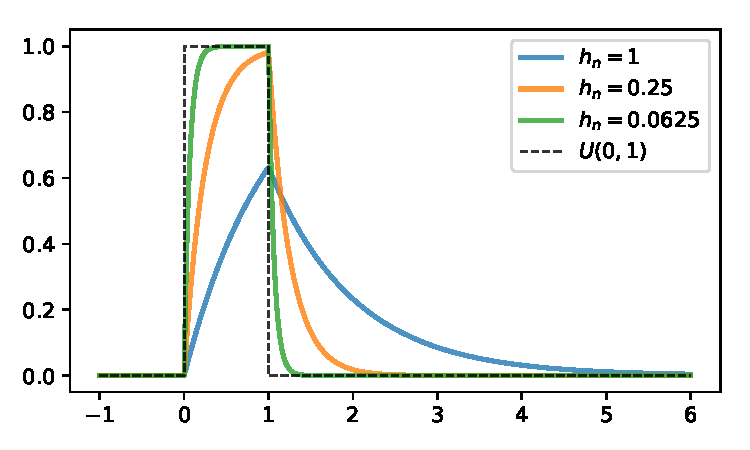
\includegraphics[width=0.5\linewidth]{figs/duda_ch4_prob3_b}
\caption{Plot of $\bar{p}(x)$ versus $x$ for $a=1$ and $h=1$, $1/4$ and $1/16$.}
\label{fig:duda_ch4_prob3_b}
\end{figure}

# The bias is $\E(p(x) - \hat{p}(x)) = p(x) - \bar{p}(x)$, and we obtain the relative bias (in percentage) by diving with $p(x)$ so that
\begin{equation*}
	\operatorname{bias}(x) = \frac{\abs{p(x) - \bar{p}(x)}}{p(x)}
	= \frac{\frac{1}{a} - \bar{p}(x)}{\frac{1}{a}} = 1 - ap(x) = e^{-x / h_n}.
\end{equation*}
The bias is decreasing on $0 < x < a$, so if we want the bias to be less than 0.01 on $99\%$ of the interval, it amounts to requiring that
\begin{equation*}
	\operatorname{bias} \left( \frac{a}{100} \right) = 0.01 
	\quad \Leftrightarrow \quad \exp \left( - \frac{a}{100 h_n} \right) = 0.01.
\end{equation*}
Solving this equation for $h_n$ reveals that $h_n = a / (100 \ln 100)$.


# When $a=0$, $h_n$ becomes $h_n = 1 / (100 \ln 100) \approx 0.0022$.
See Figure \ref{fig:duda_ch4_prob3_d} for a plot.
Although it is hard to tell exactly from the plot, observe that when $x = 0.01$, the relative bias is indeed close to $0.01$ so that $\bar{p}(0.01) = 0.99$.


\begin{figure}[ht!]
\centering
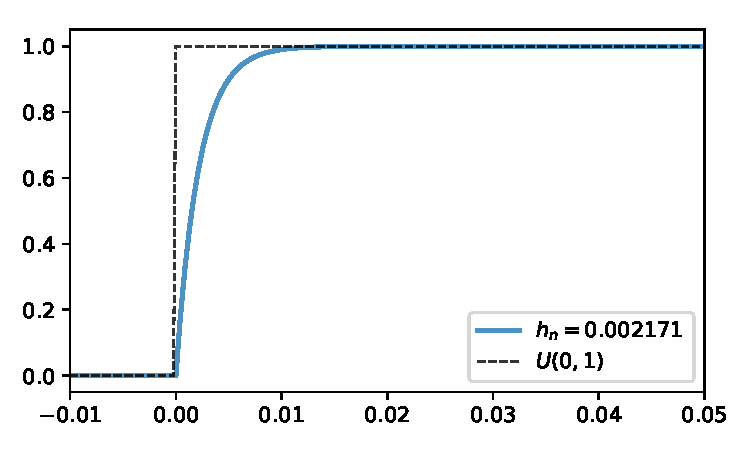
\includegraphics[width=0.5\linewidth]{figs/duda_ch4_prob3_d}
\caption{Plot accompanying problem 4.3d).}
\label{fig:duda_ch4_prob3_d}
\end{figure}

\end{easylist}







\subsubsection*{Problem 4.8}
\begin{easylist}[enumerate]
\ListProperties(Space=\listSpace, Space*=\listSpace, Numbers1=l, FinalMark1={)})
# We are given that $P(\omega_i) = 1 / c$ and 
\begin{equation*}
	p(x \mid \omega_i) = 
	\begin{dcases}
	1 & 0 \leq x \leq \frac{cr}{c-1} \\
	1 & i \leq x \leq i + 1 - \frac{cr}{c-1} \\
	0 & \text{elsewhere}
	\end{dcases}.
\end{equation*}
It helps to visualize this function.
The first line in the function definition above is for a common, overlapping region of the probability space.
The second line defines a region of the space where each category $\omega_i$ has a non-overlapping positive area of the probability density function.

In other words: the value of a random $x$ is in an overlapping part of the probability space with probability $\frac{cr}{c-1}$, and in a non-overlapping part of the space with probability $1 - \frac{cr}{c-1}$.
The value of $r$ is between $0$ and $\frac{c-1}{c}$.

Every point $x$ has a conditional probability $p(x \mid \omega_i)$ equal to 0 or 1.
To find the probability of error, we consider regions of the space with overlapping distributions, denoted $o$, and non-overlapping regions, in turn.
The Bayes error is 
\begin{align*}
	P^* &= P (\text{e})  = \int P(e \mid x) p(x) \, dx \\
	&=P (\text{e} \mid o) P (o) +
	 P (\text{e} \mid \text{not } o) P (\text{not } o ) \\
	 &= \frac{c-1}{c} \frac{cr}{c-1}  +
	 0  \left(1 - \frac{cr}{c-1} \right) = r
\end{align*}

# The nearest neighbor error rate is given by Equation (45) in Chapter 4, which is 
\begin{equation*}
	P = \int \left[1 - \sum_{i=1}^{c} P^2\left( \omega_i \mid x \right) \right]
	p(x) \, dx.
\end{equation*}
We'll integrate over the non-zero regions of the probability density.
In the non-overlapping regions, the integral becomes becomes
\begin{equation*}
	P_\text{non-overlapping} = \int \left[1 - \sum_{i=1}^{c} P^2\left( \omega_i \mid x \right) \right] p(x) \, dx
	= \int \left[1 - 1 \right]
	p(x) \, dx = 0.
\end{equation*}
This makes intuitive sense, this there is no error in non-overlapping regions in the limit of many data points.
In the overlapping regions, we have
\begin{equation*}
P_\text{overlapping}
= \int \left[1 - \sum_{i=1}^{c} \frac{1}{c^2} \right] p(x) \, dx
= \int_{0}^{\frac{cr}{c-1}} \left[1 - \frac{1}{c} \right] \, dx = r = P^*.
\end{equation*}
In other words, the Bayes error $P^*$ equals the nearest neighbor error $P$, which both equal $r$.

\end{easylist}


\subsubsection*{Problem 4.17}
We assume that $p(\omega_i) = 1/ c$ and $p(\vect{x} \mid \omega_i) = p(\vect{x})$.
In this case, for any point $\vect{x}$, any guess is as good as any other, and the Bayes error rate is clearly
\begin{equation*}
	P^* = \frac{c-1}{c}.
\end{equation*}
To prove that the bound
\begin{equation}
\label{eqn:ch4_problem17}
	P \leq P^* \left( 2 - \frac{c}{c - 1}P^* \right)
\end{equation}
is achieved, we calculate the error rate $P$.
In the following calculation, we use the fact that $p(\vect{x} \mid \omega_i) = p(\vect{x})$ and $\int p( \vect{x}) \, d\vect{x} = 1$.
We observe that
\begin{align*}
	P &= \int \left[ 1 - \sum_{i=1}^{c} P^2 \left( \omega_i \mid \vect{x} \right) \right] p( \vect{x}) \, d\vect{x} \\
	&= \int \left[ 1 - \sum_{i=1}^{c}  \left( \frac{p(\vect{x} \mid \omega_i) P( \omega_i) }{p(\vect{x})} \right)^2 \right] p( \vect{x}) \, d\vect{x} \\
	&= \int \left[ 1 - \sum_{i=1}^{c} P^2( \omega_i) \right] p( \vect{x}) \, d\vect{x} \\
	&= \left[ 1 - \sum_{i=1}^{c} \frac{1}{c^2} \right]  \int  p( \vect{x}) \, d\vect{x} \\
	&= 1 - c \frac{1}{c^2} = \frac{c-1}{c}.
\end{align*}

In other words, $P^*$ and $P$ are equal. 
When we substitute $P^*$ and $P$ into Equation \eqref{eqn:ch4_problem17}, we see that the bound is achieved since 
\begin{equation*}
	P \leq P^* \left( 2 - \frac{c}{c - 1}P^* \right) 
	\quad  \Rightarrow \quad
	\frac{c-1}{c} \leq \frac{c-1}{c} \left( 2 - \frac{c}{c-1} \frac{c-1}{c}  \right) = \frac{c-1}{c},
\end{equation*}
which completes the proof.



\subsubsection*{Problem 4.27}
\begin{easylist}[enumerate]
\ListProperties(Space=\listSpace, Space*=\listSpace, Numbers1=l, FinalMark1={)})
# Every property of a metric is easy to prove, except the triangle inequality.
I was unable to prove this.

\begin{table}[ht!]
	\centering
	\caption{Ranked order of combinations of words for problem 4.27.}
	\begin{tabular}{@{}lll@{}} \toprule
	Word 1	& Word 2 & $D_\text{Tantimoto}$ \\ \midrule
	\texttt{pots} & \texttt{stop} &  0.0 \\ 
	\texttt{pattern} & \texttt{elementary} &  0.444 \\ 
	\texttt{pattern} & \texttt{pat} &  0.5 \\ 
	\texttt{taxonomy} & \texttt{elementary} &  0.5 \\ 
	\texttt{pat} & \texttt{pots} &  0.6 \\ 
	\texttt{pat} & \texttt{stop} &  0.6 \\ 
	\texttt{pattern} & \texttt{taxonomy} &  0.7 \\ 
	\texttt{pattern} & \texttt{pots} &  0.75 \\ 
	\texttt{pattern} & \texttt{stop} &  0.75 \\ 
	\texttt{pat} & \texttt{taxonomy} &  0.75 \\ 
	\texttt{pat} & \texttt{elementary} &  0.778 \\ 
	\texttt{pots} & \texttt{taxonomy} &  0.778 \\ 
	\texttt{stop} & \texttt{taxonomy} &  0.778 \\ 
	\texttt{pots} & \texttt{elementary} &  0.909 \\ 
	\texttt{stop} & \texttt{elementary} &  0.909 \\  \bottomrule
	\end{tabular}
	\label{table:problem_4_17}
\end{table}


# There is a typo in the book, since $\binom{6}{2} = 15$.
The pairings are listed in Table \ref{table:problem_4_17} on page \pageref{table:problem_4_17}.

# Skipped this one.
\end{easylist}

\clearpage
\subsection{Linear discriminant functions}

\subsubsection*{Problem 5.4}
\begin{easylist}[enumerate]
	\ListProperties(Space=\listSpace, Space*=\listSpace, Numbers1=l, FinalMark1={)})
	# We wish to solve the problem
	\begin{align*}
	\underset{\vect{x}}{\operatorname{minimize}} \, & \norm{\vect{x} - \vect{x}_a}^2 =
		\vect{x}_a^T \vect{x}_a - 2\vect{x}^T \vect{x}_a + \vect{x}^T \vect{x} \\
		\text{subject to } \, & g(\vect{x}) = \vect{\omega}^T \vect{x} + \omega_0 = 0.
	\end{align*}
	To accomplish this, we start by constructing the Lagrange function
	\begin{equation*}
		L(\vect{x}, \lambda) = \vect{x}_a^T \vect{x}_a - 2\vect{x}^T \vect{x}_a + \vect{x}^T \vect{x} - \lambda( \vect{\omega}^T \vect{x} + \omega_0 - 0 ),
	\end{equation*}
	which we differentiate with respect to $\vect{x}$ and $\lambda$ to obtain:
	\begin{align*}
		L_{\vect{x}} &= -2 \vect{x}_a + 2 \vect{x} - \lambda \vect{\omega} = 0 \\
		L_\lambda &= \vect{\omega}^T \vect{x} + \omega_0 = 0
	\end{align*}
	We wish to solve these equations for $\vect{x}$.
	
	Solving the first equation for $\vect{x}$ yields $\vect{x} = \lambda \vect{\omega} / 2 + \vect{x}_a$.
	It remains to solve for $\lambda$.
	If we left-multiply by $\vect{\omega}^T$ and compare with the second equation, we observe that
	\begin{equation*}
		\vect{\omega}^T \vect{x} 
		= -\omega_0 \quad \text{and} 
		\quad 
		\vect{\omega}^T \vect{x} 
		= 
		\frac{\norm{\vect{\omega}}^2 \lambda}{2} + \vect{\omega}^T \vect{x}_a.
	\end{equation*}
	This implies that
	\begin{equation*}
		-\omega_0 =  \frac{\norm{\vect{\omega}}^2 \lambda}{2} + \vect{\omega}^T \vect{x}_a \quad \Leftrightarrow \quad \lambda = - \frac{2}{\norm{\vect{\omega}}^2}\left( \omega_0 + \vect{\omega}^T \vect{x}_a \right),
	\end{equation*}
	and substituting this into $\vect{x} = \lambda \vect{\omega} / 2 + \vect{x}_a$ yields the optimal answer
	\begin{equation}
	\label{eqn:ch5_prob4}
		\vect{x}^* = -\frac{\vect{\omega}}{\norm{\vect{\omega}}^2} \left( \vect{\omega}^T \vect{x}_a + \omega_0 \right) + \vect{x}_a = - \frac{\vect{\omega}}{\norm{\vect{\omega}}^2} g(\vect{x}_a) + \vect{x}_a.
	\end{equation}
	Inserting this into $\norm{\vect{x}^* - \vect{x}_a}$ yields 
	\begin{equation*}
		\norm{\vect{x}^* - \vect{x}_a}=
		\norm{\frac{\vect{\omega}}{\norm{\vect{\omega}}^2} g(\vect{x}_a)}
		= \frac{\abs{g(\vect{x}_a)}}{\norm{\vect{\omega}}}.
	\end{equation*}
	
	# The projection onto the plane is the minimizer $\vect{x}^*$ from Equation \eqref{eqn:ch5_prob4} in the previous sub-problem, so we immediately see that 
	\begin{equation*}
	\vect{x}^* = -\frac{\vect{\omega}}{\norm{\vect{\omega}}^2} \left( \vect{\omega}^T \vect{x}_a + \omega_0 \right) + \vect{x}_a = - \frac{\vect{\omega}}{\norm{\vect{\omega}}^2} g(\vect{x}_a) + \vect{x}_a
	=  
	\vect{x}_a - \frac{g(\vect{x}_a)}{\norm{\vect{\omega}}^2}  \vect{\omega},
	\end{equation*}
	which is what we were required to show.
\end{easylist}

\subsubsection*{Problem 5.13}
We wish to choose $\eta(k)$ to minimize the quadratic function
\begin{equation*}
	J \left( \vect{a}(k+1)  \right)
	\simeq
	J \left( \vect{a}(k)  \right)
	-
	\eta(k) \norm{\nabla \vect{J}}^2
	+
	\frac{1}{2} \eta^2(k) \nabla \vect{J}^T \vect{H} \nabla \vect{J}.
\end{equation*}
Differentiating and setting the result equal to zero yields
\begin{equation*}
	\frac{\partial J \left( \vect{a}(k+1)  \right)}{\partial \eta(k)}
	=
	-
	\norm{\nabla \vect{J}}^2
	+
	\eta(k) \nabla \vect{J}^T \vect{H} \nabla \vect{J} = 0,
\end{equation*}
and solving this equation for $\eta(k)$ yields the desired answer, which is
\begin{equation*}
	\eta(k) = \frac{\norm{\nabla \vect{J}}^2}{\nabla \vect{J}^T \vect{H} \nabla \vect{J}}.
\end{equation*}

\subsubsection*{Problem 5.15}
\begin{easylist}[enumerate]
	\ListProperties(Space=\listSpace, Space*=\listSpace, Numbers1=l, FinalMark1={)})
	#
If $\alpha > \beta^2 / 2 \gamma$, then $-2 \alpha \gamma +\beta^2 < 0$ and 
\begin{equation*}
	\norm{\vect{a}(k+1) - \alpha \hat{\vect{a}}}^2 
	\leq
	\norm{\vect{a}(k) - \alpha \hat{\vect{a}}}^2 - 2 \alpha \gamma +\beta^2
\end{equation*}
represents error which decreases at each step.
After $k$ corrections we obtain
\begin{equation*}
\norm{\vect{a}(k+1) - \alpha \hat{\vect{a}}}^2 
\leq
\norm{\vect{a}(1) - \alpha \hat{\vect{a}}}^2 + k(-2 \alpha \gamma +\beta^2),
\end{equation*}
and the error is zero when $\norm{\vect{a}(1) - \alpha \hat{\vect{a}}}^2 + k_0(-2 \alpha \gamma +\beta^2) = 0$, which implies that
\begin{equation*}
	k_0 = \frac{\norm{\vect{a}(1) - \alpha \hat{\vect{a}}}^2}{2 \alpha \gamma - \beta^2}.
\end{equation*}
This is what we were asked to show.

# Skipped. Somehow I did not see this problem when originally solving.
\end{easylist}

\subsubsection*{Problem 5.21}
To ease the notation, let us write $\vect{m} := \vect{m}_1 - \vect{m}_2$\footnote{This definition of $\vect{m}$ is not the same as the one used in the book, where $\vect{m}$ is the grand mean.}.
Staring with Equation (53) from Chapter 5 in \cite{duda_pattern_2000}, we left-multiply by the bracketed term to isolate $\vect{w}$ as 
\begin{equation}
\label{eqn:ch5_prob21}
	\vect{w} = \left[ \frac{1}{n} \vect{S}_W + \frac{n_1 n_2}{n^2} \vect{m} \vect{m}^T \right]^{-1} \vect{m}.
\end{equation}
Recall from Problem 3.36 that the Sherman-Morrison-Woodbury matrix identity is 
\begin{equation*}
	\left(\vect{A} + \vect{x}\vect{y}^T\right)^{-1} =
	\vect{A}^{-1} - \frac{\vect{A}^{-1} \vect{x} \vect{y}^t \vect{A}^{-1}}{1 + \vect{y}^T \vect{A}^{-1} \vect{x}}.
\end{equation*}
We now apply the identity to the bracketed term in Equation \eqref{eqn:ch5_prob21}.
In doing so, we identify 
\begin{equation*}
	\vect{A} \cong \frac{1}{n} \vect{S}_W 
	\quad \quad \text{and} \quad \quad
	\vect{x}\vect{y}^T \cong \frac{n_1 n_2}{n^2} \vect{m} \vect{m}^T.
\end{equation*}
Applying the matrix identity, we obtain
\begin{align*}
	\vect{w} &= \left[ n \vect{S}_W^{-1} - \frac{
		n^2 \left( \frac{n_1 n_2}{n^2} \right)
		\vect{S}_W^{-1} \vect{m} \vect{m}^T \vect{S}_W^{-1}
		}{
		1 + n \left( \frac{n_1 n_2}{n^2} \right) \vect{m}^T \vect{S}_W^{-1} \vect{m} 
		}  \right] \vect{m} \\
		&=
		n \vect{S}_W^{-1}\vect{m} - \frac{
			n \left( \frac{n_1 n_2}{n} \right)
			\vect{S}_W^{-1} \vect{m} \vect{m}^T \vect{S}_W^{-1}\vect{m}
		}{
		1 +  \left( \frac{n_1 n_2}{n} \right) \vect{m}^T \vect{S}_W^{-1} \vect{m} 
	}.
\end{align*}
To simplify the notation and remind ourselves that some of these quantities are simply scalars, let us denote $a:= n_1 n_2 / n$ and $b := \vect{m}^T \vect{S}_W^{-1} \vect{m} $.
We simplify and factor our $n \vect{S}_W^{-1} \vect{m}$ to obtain
\begin{equation*}
	\vect{w} = n \vect{S}_W^{-1}\vect{m} - \frac{
		n a
		\vect{S}_W^{-1} \vect{m} b
	}{
	1 +  a b }
	=
	n \vect{S}_W^{-1} \vect{m} \left[ 1  - \frac{ab}{1 + ab} \right]
	=
	n \vect{S}_W^{-1} \vect{m} \left[ 1  + ab \right]^{-1}.
\end{equation*}
Recalling now that $a:= n_1 n_2 / n$ and $b := \vect{m}^T \vect{S}_W^{-1} \vect{m} $, we have accomplished the goal.
The result is that
\begin{equation*}
	\vect{w} = n \vect{S}_W^{-1} \vect{m} \alpha = n \vect{S}_W^{-1} \vect{m} \big[ 1 + \underbrace{\left( \frac{n_1 n_2}{n} \right)}_a \underbrace{\vect{m}^T \vect{S}_W^{-1} \vect{m}}_b \big]^{-1},
\end{equation*}
which shows that $\alpha$ is indeed given by the quantity in the problem statement.

\subsubsection*{Problem 5.25}
\begin{easylist}[enumerate]
\ListProperties(Space=\listSpace, Space*=\listSpace, Numbers1=l, FinalMark1={)})

# We supply a proof by induction: we first show the base case, and then the inductive step.

\textbf{The base case} is verified by checking that the relation holds for $\eta^{-1}(2) = \eta^{-1}(1) + y_1^2$.
This is true, since it implies
\begin{equation*}
	\eta(2) = \frac{1}{\eta^{-1}(1) + y_1^2}
	= \frac{\eta(1)}{1 + \eta(1) y_1^2}
	= \frac{\eta(1)}{1 + \eta(1) \sum_{i=1}^{1}y_i^2},
\end{equation*}
which is clearly the given formula for $k = 2$.

In \textbf{the inductive step} we assume that the relation holds for $\eta(k)$, and show that this implies that it holds for $\eta(k+1)$ too.
The required algebra is
\begin{align*}
	\eta^{-1}(k+1) &= \eta^{-1}(k) + y_k^2 \\
&= \left( \frac{\eta(1)}{1 + \eta(1) \sum_{i=1}^{k-1}y_i^2 }  \right)^{-1} + y_k^2 \\
&= \frac{1 + \eta(1) \sum_{i=1}^{k-1}y_i^2}{\eta(1) } + \frac{\eta(1)}{\eta(1)}y_k^2 \\
&= \frac{1 + \eta(1) \sum_{i=1}^{k}y_i^2}{\eta(1)}.
\end{align*}
Inverting this shows that $\eta(k+1) = \eta(1) / \left( 1 + \eta(1) \sum_{i=1}^{k}y_i^2 \right)$, as required.



# To show why the sequence of coefficients will satisfy the sums, we will first bound the terms, and the convert the problems to integrals.

If $0 < a \leq y_i^2 \leq b < \infty$ for every $i$, then the sum is bounded by
\begin{equation*}
	a(k-1) \leq \sum_{i=1}^{k-1} y_i^2 \leq b(k-1),
\end{equation*}
and this in turn implies the expression $\eta(k)$ that may be bounded by
\begin{equation*}
	\frac{\eta(1)}{1 + \eta(1) b(k-1)} \leq \eta(k) \leq\frac{\eta(1)}{1 + \eta(1) a(k-1)}.
\end{equation*}

To show that $\sum \eta(k) \to \infty$, we note that $\sum \eta(k) \simeq \lim_{\alpha \to \infty} \int_{x=1}^{x=\alpha} \eta(x) \, dx $.
We observe that the integral
\begin{equation*}
	\lim_{\alpha \to \infty} \int_{x=1}^{x=\alpha} \frac{\eta(1)}{1 + \eta(1)(x-1)b} \, dx 
	= 
	\lim_{\alpha \to \infty} \left. \frac{1}{b} \ln \abs{u} \right|_{u=1}^{u=1 + \eta(1) (\alpha - 1)b}
\end{equation*}
diverges for any value of $b$, where we used the substitution $u = 1 + \eta(1)(x-1)b$.
Since $b$ represents the maximal value of the terms $\eta(k)$, any other value of $y_i^2$ will diverge too, and the sum $\sum \eta(k)$ diverges to infinity.

To show that $\sum \eta^2(k) \to L < \infty$, we again use $\sum \eta^2(k) \simeq \lim_{\alpha \to \infty} \int_{x=1}^{x=\alpha} \eta^2(x) \, dx $.
Now the integral converges, since for any value of $a$ the integral
\begin{equation*}
\lim_{\alpha \to \infty} \int_{x=1}^{x=\alpha} \frac{\eta^2(1)}{(1 + \eta(1)(x-1)b)^2} \, dx 
= 
\lim_{\alpha \to \infty} \left. \frac{\eta(1)}{bu} \right|_{u=1 + \eta(1) (\alpha - 1)a}^{u=1} \leq \frac{\eta(1)}{b}
\end{equation*}
converges, and $a$ represents the maximal bound on $\eta(k)$. 
The sum $\sum \eta(k)$ diverges to infinity, for any $0 < a \leq y_i^2 \leq b < \infty$.
\end{easylist}




\subsubsection*{Problem 5.27}
\begin{easylist}[enumerate]
\ListProperties(Space=\listSpace, Space*=\listSpace, Numbers1=l, FinalMark1={)})
# The data points are plotted in Figure \ref{fig:duda_ch5_prob27} on page \pageref{fig:duda_ch5_prob27}, and as seen in the plot they are not linearly separable.


\begin{figure}[ht!]
	\centering
	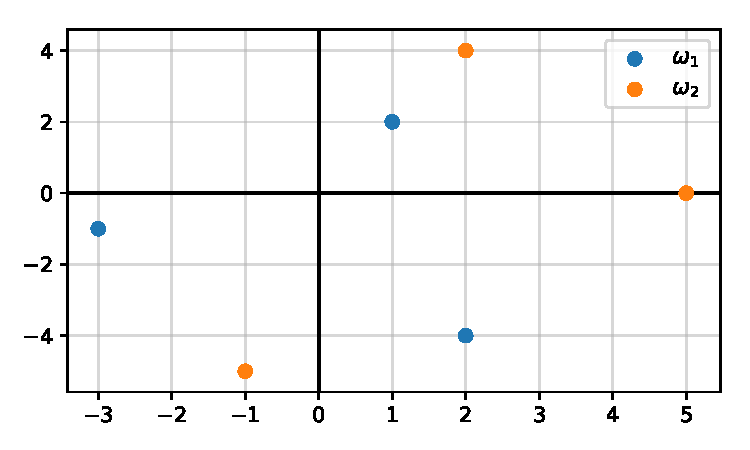
\includegraphics[width=0.5\linewidth]{figs/duda_ch5_prob27}
	\caption{Graf accompanying problem 5.27.}
	\label{fig:duda_ch5_prob27}
\end{figure}


# From Equation (95) we observe that the optimal choice of $\eta$ is given by

\begin{equation*}
	\eta(k) = \frac{\norm{\vect{Y}^T \abs{\vect{e}(k)}}^2}
	{\norm{\vect{Y}\vect{Y}^T \abs{\vect{e}(k)}}^2}
	= \frac{\vect{e}^T \vect{Y} \vect{Y}^T \vect{e}}
	{\vect{e}^T \vect{Y} \vect{Y}^T \vect{Y} \vect{Y}^T \vect{e}}.
\end{equation*}
This value varies from loop to loop, depending on $\vect{e}$.
For this specific data set, the value of $\vect{Y}$ and $\vect{Y} \vect{Y}^T$ are given in equation \eqref{eqn:chapter5_prob27}.

\begin{gather*}
\label{eqn:chapter5_prob27}
	\vect{Y} = \left(\begin{matrix}
	1.0 & 1.0 & 2.0\\1.0 & 2.0 & -4.0\\1.0 & -3.0 & -1.0\\-1.0 & -2.0 & -4.0\\-1.0 & 1.0 & 5.0\\-1.0 & -5.0 & 0.0
	\end{matrix}\right)
	\\
	\vect{Y} \vect{Y}^T = 
	\left(\begin{matrix}
	6.0 & -5.0 & -4.0 & -11.0 & 10.0 & -6.0\\-5.0 & 21.0 & -1.0 & 11.0 & -19.0 & -11.0\\-4.0 & -1.0 & 11.0 & 9.0 & -9.0 & 14.0\\-11.0 & 11.0 & 9.0 & 21.0 & -21.0 & 11.0\\10.0 & -19.0 & -9.0 & -21.0 & 27.0 & -4.0\\-6.0 & -11.0 & 14.0 & 11.0 & -4.0 & 26.0
	\end{matrix}\right)
\end{gather*}

\begin{figure}[ht!]
	\centering
	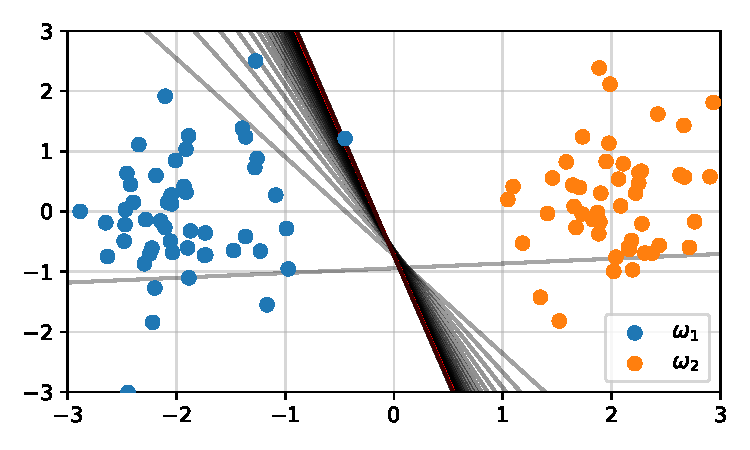
\includegraphics[width=0.5\linewidth]{figs/duda_ch5_prob27_b}
	\caption{Convergence of the Ho Kashyap algorithm.}
	\label{fig:duda_ch5_prob27_b}
\end{figure}

\end{easylist}


\subsubsection*{Problem 5.29}
To show that there always exists a mapping to a higher dimensional space which leaves points from two classes linearly separable, we will explicitly provide such a mapping.
The mapping would be very inefficient in practice, but provides a constructive proof.

Observe first that to apply a linear classifier to points where data from one class is close to the origin, a function such as $y = \phi (\vect{x}) = \exp(- \vect{x}^T \vect{x})$ may be used.
This leaves the data linearly separable in the new space, as illustrated in Figure \ref{fig:1024px_Kernel_trick_idea_svg_wikipedia}.
Below we will extend this idea by introducing many distinct mappings $\phi (\vect{x})$.
\begin{figure}
	\centering
	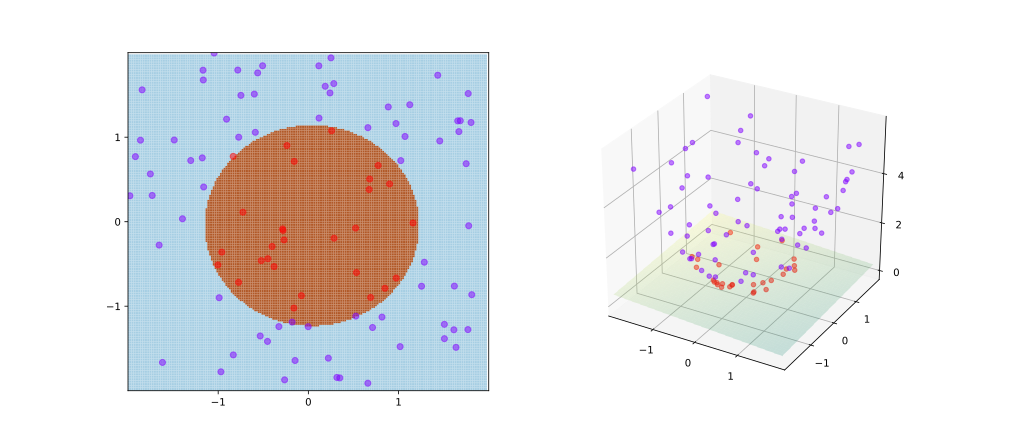
\includegraphics[width=0.85\linewidth]{figs/1024px_Kernel_trick_idea_svg_wikipedia}
	\caption{Using a kernel to raise points in a new dimension. Source: \url{https://commons.wikimedia.org/wiki/File:Kernel_trick_idea.svg}}
	\label{fig:1024px_Kernel_trick_idea_svg_wikipedia}
\end{figure}

Consider now points $\D = \left\{ \vect{x}_1, \vect{x}_2, \dots, \vect{x}_N \right\}$ in $\R^d$.
Assume that some points $S \subseteq \D$ belong to $\omega_1$, and that we know exactly which points. 
If we know which points belong to  $\omega_1$, then a kernel density estimate  (Parzen window) such as
\begin{equation*}
	y  = \operatorname{Parzen}(S) = \frac{1}{\abs{S}}\sum_{\vect{x}_i \in S} \frac{1}{h} \phi \left( \frac{\vect{x} - \vect{x}_i}{h} \right)
\end{equation*}
with a sufficiently small value of the bandwidth $h$ will raise these points in the new $y$ feature space.
When $h \ll 1$, neighboring points not belonging to $\omega_1$ will be unaffected.
A plane such as $y = 0.1$ will then perfectly separate the points.

Since we do not know the true subset $S \subseteq \D$, we can apply this transformation on \emph{every} possible subset of $\D$ (the \emph{power set} of $\D$).
There are $2^{\abs{S}}$ such subsets.
We use
\begin{equation*}
	\vect{y} = 
	\begin{pmatrix}
	\vect{x} & \operatorname{Parzen}(S_1) & \operatorname{Parzen}(S_1) & \dots & \operatorname{Parzen}(S_{2^{\abs{S}}})
	\end{pmatrix}
\end{equation*}
to map $\vect{x} \in \R^d$ to a $d + 2^{\abs{S}$ space.
In other words: if $\left\{ \vect{x_1} \right\}$ is ``raised'' in one new feature dimension, $\left\{ \vect{x_1}, \vect{x_2} \right\}$ in another, $\left\{ \vect{x_1}, \vect{x_3} \right\}$ in yet another, etc. for \emph{every} combination of points, then in some dimension in the feature space the points are linearly separable.






\subsubsection*{Problem 5.32}
\begin{easylist}[enumerate]
\ListProperties(Space=\listSpace, Space*=\listSpace, Numbers1=l, FinalMark1={)})
# The plot is show in Figure \ref{fig:duda_ch5_prob32}.
By inspection the weight vector is 
\begin{equation*}
	\vect{a} = (a_0, a_1, a_2)= (-1.5, 1, 1).
\end{equation*}
This corresponds to the line $y = 1.5 - x$.
The optimal margin is the distance from the line $y = 1.5 - x$ to a point, say $(1,1)$, and this distance is $\sqrt{2}/4 \approx 0.3536$.

\begin{figure}[ht!]
	\centering
	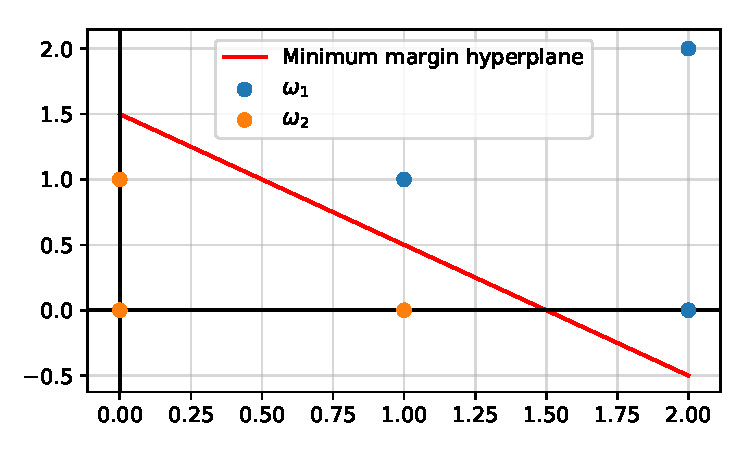
\includegraphics[width=0.5\linewidth]{figs/duda_ch5_prob32}
	\caption{Plot related to problem 5.32a).}
	\label{fig:duda_ch5_prob32}
\end{figure}

# From inspection there are four support vectors, and they are
\begin{align*}
	(0, 1)^T \quad & \quad (1, 0)^T \\
	(1, 1)^T \quad & \quad (2, 0)^T.
\end{align*}

# This laborious computation is omitted.


\end{easylist}




\subsubsection*{Problem 5.33}
\begin{easylist}[enumerate]
\ListProperties(Space=\listSpace, Space*=\listSpace, Numbers1=l, FinalMark1={)})
# The optimization problem
\begin{equation}
\label{eqn:ch5_problem_33_1}
	L(\vect{a}, \vect{\alpha}) = \frac{1}{2} \norm{\vect{a}}^2 -
	\sum_{k=1}^{n} \alpha_k \left[ z_k \vect{a}^T \vect{y}_k - 1 \right]
\end{equation}
has a solution which is a saddle point, since we wish to maximize with respect to $\vect{\alpha}$ and minimize with respect to $\vect{a}$.

# Here I believe there to be a slight error in the text, which might lead to confusion.
In the initial pages of the chapter, the distance from a point to a hyperplane is given by $r = (\vect{\omega}^T \vect{x} + \omega_0) / \norm{\vect{\omega}}$, and this is indeed correct.

In the context of SVMs, however, the distance is said to be 
\begin{equation*}
	\frac{g(y)}{\norm{\vect{a}}}
	=
	\frac{\vect{a} ^T \vect{y}}{\norm{\vect{a}}}
	=
	\frac{(\omega_0, \vect{a}') (1, \vect{y}')^T}{\norm{\vect{a}}}
	=
	\frac{\vect{a}'\,^T\vect{y} + \omega_0}{\norm{\vect{a}}},
\end{equation*}
which is different because $\vect{a}$ is in the denominator, not $\vect{a}'$.
Amending Equation \eqref{eqn:ch5_problem_33_1} with this information, the $\frac{1}{2} \norm{\vect{a}}^2$ should be replaced by $\frac{1}{2} \norm{\vect{a}'}^2$, i.e. dropping $\vect{a}_0 = \omega_0$.
If we do this and differentiate with respect to the first component of $\vect{a}$, we obtain
\begin{equation*}
	\frac{\partial L(\vect{a}, \vect{\alpha})}{\partial \vect{a}_0}
	=
	\sum_k \alpha_k^* z_k \vect{y}_0 = 0,
\end{equation*}
which gives the desired result since $\vect{y}_0 = 1$ due to the augmentation of the vector.

# To prove this, we differentiate with respect to $\vect{a}$ and obtain
\begin{equation*}
\frac{\partial L(\vect{a}, \vect{\alpha})}{\partial \vect{a}}
=
\vect{a}^* - \sum_k \alpha_k^* z_k \vect{y}_k = 0.
\end{equation*}

# If the Lagrange multiplier (or \emph{undetermined multiplier}) $\alpha_k^*$ is zero, then it's said to be \emph{inactive}.
At the optimum, the constraint is not used.
The optimum of $L(\vect{a}, \vect{\alpha})$ is then the same with or without this constraint.

If the Lagrange  multiplier $\alpha_k^*$ is non-zero, then the constraint is said to be \emph{active}.
The constrained solution is different from the unconstrained solution, and the optimum lies on the boundary of the constraint.
Since $\alpha_k^* z_k \vect{y}_k \geq 1$ in the feasible region, the optimal solution is on the boundary if $\alpha_k^* z_k \vect{y}_k = 1$, but then  $\alpha_k^*$ is non-zero since the constraint is active.

In conclusion, either $\alpha_k^* z_k \vect{y}_k = 1$ if the constraint is active, or $\alpha_k^* = 0$ if the constraint is inactive.
This is one of the Karush–Kuhn–Tucker (KKT) conditions, and it may be expressed as
\begin{equation*}
	\alpha_k^* \left[ \alpha_k^* z_k \vect{y}_k - 1 \right] = 0 \qquad k = 1 , \dots, n.
\end{equation*}

# We simply multiply the brackets in Equation \eqref{eqn:ch5_problem_33_1} from subproblem a).
\begin{equation*}
L(\vect{a}, \vect{\alpha}) = \frac{1}{2} \norm{\vect{a}}^2 -
\sum_{k=1}^{n} \alpha_k \left[ z_k \vect{a}^T \vect{y}_k - 1 \right]
=
\frac{1}{2} \norm{\vect{a}}^2 -
\sum_{k=1}^{n} \alpha_k  z_k \vect{a}^T \vect{y}_k 
+
\sum_{k=1}^{n} \alpha_k 
\end{equation*}

# Using $\vect{a}^* = \sum_j \alpha_j^* z_j \vect{y}_j$ we observe that
\begin{align*}
	L(\vect{\alpha}) &= 
	\frac{1}{2} \norm{\vect{a}^*}^2 -
	\sum_{k=1}^{n} \alpha_k  z_k \vect{a}^{*T} \vect{y}_k 
	+
	\sum_{k=1}^{n} \alpha_k \\
	&= 
	\frac{1}{2} 
	\left(\sum_j \alpha_j^* z_j \vect{y}^T_j\right)
	\left(\sum_k \alpha_k^* z_k \vect{y}_k\right)
	 -
	\sum_{k=1}^{n} \alpha_k  z_k 
	\left(\sum_j \alpha_j^* z_j \vect{y}^T _j\right)
	\vect{y}_k 
	+
	\sum_{k=1}^{n} \alpha_k 
\end{align*}
and since the first and second terms are equal, we obtain
\begin{equation*}
-
\frac{1}{2} 
\left(\sum_j \alpha_j^* z_j \vect{y}^T_j\right)
\left(\sum_k \alpha_k^* z_k \vect{y}_k\right)
+
\sum_{k=1}^{n} \alpha_k 
= 
-
\frac{1}{2} 
\sum_j \sum_k \alpha_j^* \alpha_k^* z_j z_k \vect{y}_j^T \vect{y}_k
+
\sum_{k=1}^{n} \alpha_k 
\end{equation*}
as desired.
We have formulated the problem as a maximization over $L(\vect{\alpha})$.
\end{easylist}





\clearpage
\subsection{Multilayer Neural Networks}

\subsubsection*{Problem 6.5}
The backpropagation rule for input-to-hidden weights is given by Equation (21), which is
\begin{equation*}
	\Delta w_{ji} =
	\eta \delta_j x_i = 
	\eta \left[ \sum_{k=1}^{c} w_{kj} \delta_k \right] f'(\text{net}_j) x_i.
\end{equation*}
Notice that if $z_k = t_k$ for every value of $k$, there is nothing to learn since the error is zero.
In this case, $\delta_k = 0$ and as a result $\Delta w_{ji} = 0$.
The learning rate is proportional to the error $(t_k - z_k)$, but it's also weighted by $w_{kj}$.
The higher this weight is, the more an error contributes and the further it is adjusted in the backpropagation rule.



\subsubsection*{Problem 6.8}
\begin{easylist}[enumerate]
\ListProperties(Space=\listSpace, Space*=\listSpace, Numbers1=l, FinalMark1={)})
# In this problem it helps to make a drawing, or study Figures 6.4 and 6.2 in the book.

\begin{easylist}
	\ListProperties(Space=\listSpace, Space*=\listSpace, Numbers2=r, FinalMark1={)})
## The bias is connected to $n_H + c$ weights.
## Every one of the $d$ inputs is connected to every one of the $n_H$ hidden units, for a total of $d n_H$ weights.
## Every hidden unit $n_H$ is connected to every one of the $c$ outputs, for $n_H c$ weights. 
\end{easylist}



The total number of weights is therefore given by
\begin{equation*}
	n_H + c + d n_H  +n_H c = n_H (1 + d + c) + c.
\end{equation*}

# Consider the equation
\begin{equation*}
	z_k = f\left[
	\sum_{j=1}^{n_H} w_{kj} \, f \left( \sum_{i=1}^{d} w_{ji} x_i + w_{j0} \right) + w_{k0}
	\right]
\end{equation*}
for a neural network output.
If the sign is flipped on every weight going into a hidden unit, and the weights leading out from that same unit are also flipped, then the net result is no change if the activation function obeys $f(-x) = -f(x)$.
In other words, if the $w_{ji} \mapsto -w_{ji}$ and $w_{j0} \mapsto - w_{j0}$ in the equation above, then 
\begin{equation*}
	f \left( \sum_{i=1}^{d} -w_{ji} x_i - w_{j0} \right) = -f \left( \sum_{i=1}^{d} w_{ji} x_i + w_{j0} \right)
\end{equation*}
and a mapping $w_{kj} \mapsto -w_{kj}$ in the outer sum will cancel the sign flip.
Note that this result only applies to odd functions where $f(-x) = -f(x)$.

# If there are $n_H$ hidden units, there are $n_H!$ ways to permute them.
For each of these permutations, every associated weight might have it's sign flipped or not, for a total of $2^{n_H}$ possibilities with respect to sign flipping.
The total count is therefore $n_H! 2^{n_H}$ exchange symmetries (not $n_H 2^{n_H}$ as \cite{duda_pattern_2000} claims).
This result is verified in \cite{bishop_pattern_2011} on page 232, so we assume that \cite{duda_pattern_2000} contains a typo here and the ``!'' sign was forgotten.

\end{easylist}

\subsubsection*{Problem 6.10}
\begin{easylist}[enumerate]
	\ListProperties(Space=\listSpace, Space*=\listSpace, Numbers1=l, FinalMark1={)})
	# The rules of differentiation in calculus shows that when $f(x) = 1 /(1 + e^{ax} )$, then the derivative may be expressed in terms of the function as
	\begin{equation*}
		f'(x) = -a e^{ax} f^2(x).
	\end{equation*}
	
	# We'll study $f(x) = a (1 - e^{-2bx}) / (1 + e^{-2bx})$, and it pays off to ease notation somewhat.
	Letting $g(x) := e^{-2bx}$, we have $g'(x) = -2b g(x)$ and we expedite notation by writing
	\begin{equation*}
		f(x) = a \frac{1 - e^{-2bx}}{1 + e^{-2bx}} :=
		a \frac{1 - g(x)}{1 + g(x)} =  a (1 - g(x)) (1 + g(x))^{-1}.
	\end{equation*}
	Differentiating this and using the chain rule and product rule of calculus, we obtain
	\begin{align*}
		f'(x) &=  \frac{-a g'(x) (1 + g(x)) - ag'(x) (1 - g(x))}{(1 + g(x))^2} \\
		&= \frac{4 ab g(x)}{(1 + g(x))^2} = \underbrace{a \frac{1 - g(x)}{1 + g(x)}}_{f'(x)} \frac{4bg(x)}{(1 - g(x)) (1 + g(x))}.
	\end{align*}
	Substituting back $g(x) := e^{-2bx}$, we see that  the derivative may be expressed in terms of the function as
	\begin{equation*}
		f'(x) = f(x) \frac{4 b  e^{-2bx}}{1 - e^{-4bx}}.
	\end{equation*}
\end{easylist}


\subsubsection*{Problem 6.16}
\begin{easylist}[enumerate]
\ListProperties(Space=\listSpace, Space*=\listSpace, Numbers1=l, FinalMark1={)})
# Without loss of generality we assume that $J(\vect{w}) = \frac{1}{2}\vect{w}^T \vect{H} \vect{w}$, since by a transformation of the type $\vect{w} = \vect{w}' - \vect{c}$ we could transform a general, non-centered quadratic equation to this form.
This is analogous to scaling $f(x) = a x^2 + bx + x$ in order to formulate it as $f(x') = a' x'^2$.

To study convergence, we examine the learning rule, which may be written as
\begin{align*}
	\vect{w}_{n+1} &= \vect{w}_{n} - \eta \nabla J(\vect{w}_{n}) \\
	&= \vect{w}_{n} - \eta  \vect{H} \vect{w}_{n} \\
	&=  \left( \vect{I} - \eta  \vect{H} \right) \vect{w}_{n},
\end{align*}
and observe that $\vect{w}_{n} = \left( \vect{I} - \eta  \vect{H} \right)^n \vect{w}_{0}$.
Convergence is ensured if $\left( \vect{I} - \eta  \vect{H} \right)^n$ goes to zero as $n \to \infty$.
Informally, repeated application of the matrix should bring the vector to zero.
The convergence of repeated application of a matrix to a vector is controlled by eigenvectors and eigenvalues.

We write $\left( \vect{I} - \eta  \vect{H} \right) = \vect{Q} \vect{\Lambda} \vect{Q}^T$ to express the symmetric, positive definite matrix in it's eigenvalue decomposition.
Then we define $\vect{w}_{k}' = \vect{Q} \vect{w}_{k} = \sum_{i=1}^{d} \alpha_i \vect{v}_i$ to express $\vect{w}_{k}$ in the \emph{eigenvalue basis} of $\vect{H}$, where the $\vect{v}_i$s are the orthonormal eigenvectors. 
This transformation is a rotation of the space, since $\vect{Q}$ is orthonormal.

The expression on the left below is for the vector, and the expression on the right captures the behavior of a single eigenvector component $\vect{v}_i$.
\begin{equation*}
	\left(\sum_{i=1}^{d} \alpha_i \vect{v}_i\right)_{n+1} = \vect{Q} \vect{\Lambda} \left(\sum_{i=1}^{d} \alpha_i \vect{v}_i\right)_{n}
	\quad \Leftrightarrow \quad
	(\alpha_i \vect{v}_i)_{n+1} = \vect{Q} \lambda_i (\alpha_i \vect{v}_i)_{n+1}
\end{equation*}
The matrix $\vect{Q}$ is orthogonal, so it merely rotates or reflects a vector, but $\norm{\vect{v}_i} = \norm{\vect{Q} \vect{v}_i}$ so the magnitude is unchanged.
Therefore we ignore it when considering convergence, and see that learning is ensured if $\abs{\lambda_i} < 1$ for every $i=1, 2, \dots, d$.
Since every eigenvalue is positive, the maximal eigenvalue controls convergence.

The only thing left to do is to relate the eigenvalues of $\left( \vect{I} - \eta  \vect{H} \right)$ to the eigenvalues of $ \vect{H}$.
If a matrix is multiplied by a scalar, then so are it's eigenvalues.
The effect of subtraction by the identity matrix is not as obvious, but if we write out the equation for the characteristic polynomials we observe that
\begin{align*}
	\text{eig. vals of } \left( \vect{I} - \eta  \vect{H} \right) \, &\Leftrightarrow \, \text{ zeros of } \det \left(  \vect{I} -  \eta  \vect{H} - \lambda \vect{I} \right)
	=
	\det \left(  \vect{I} (1 - \lambda ) - \eta  \vect{H} \right)
	 \\
	\text{eig. vals of } \eta  \vect{H} \, &\Leftrightarrow \, \text{ zeros of } \det \left(  \vect{I} \lambda'  - \eta   \vect{H} \right),
\end{align*}
and comparing we observe that $\lambda' = \lambda - 1$.
We're really after the eigenvalues of $\vect{H}$, which we'll now denote by $\lambda_{\vect{H}} = \lambda' / \eta$.
From this, we have convergence if
\begin{align*}
	-1 < &\lambda_{\text{max}} < 1 \\
	-1 < &1 - \eta \lambda_{\vect{H} \text{max}} < 1 \\
	\eta \lambda_{\vect{H} \text{max}} &< 2,
\end{align*}
which is the same as requiring that $\eta < \lambda_{\vect{H} \text{max}} / 2$.

# The best learning rate is achieved if we manage to choose $\eta$ such that the maximal eigenvalue (in absolute value) of $\left( \vect{I} - \eta  \vect{H} \right)$ is close to zero.
The optimal rate is given by\footnote{See \url{https://distill.pub/2017/momentum/} for details.}
\begin{equation*}
	\text{rate}(\eta) = \max_i \abs{1 - \eta \lambda_i}
	= \max \left( \abs{1 - \eta \lambda_1} , \abs{1 - \eta \lambda_d}\right)
\end{equation*}
where $\lambda_1$ is the smallest eigenvalue of $\vect{H}$ and $\lambda_d$ is the largest.
Convergence is fastest when these arguments are equal in absolute value, so we require that
\begin{equation*}
	(1 - \eta \lambda_1) = - (1 - \eta \lambda_d)
\end{equation*}
and solve for $\eta$ to obtain $\eta^*= 2 / (\lambda_1 + \lambda_d)$.
The optimal learning rate is obtained by substituting this $\eta^*$ into the function $\text{rate}(\cdot)$.
We consider the positive value $(1 - \eta^* \lambda_1)$, which becomes
\begin{equation*}
	\text{rate}(\eta^*) = (1 - \eta^* \lambda_1) = \frac{\lambda_d - \lambda_1}{\lambda_d + \lambda_1} = \frac{ \lambda_d / \lambda_1 - 1}{\lambda_d / \lambda_1 + 1},
\end{equation*}
and recognize that the learning rate is indeed dependent on the ratio of the largest to the smallest eigenvalue of $\vect{H}$.

# An informal argument is as follows: Consider unstandardized data which is not highly correlated (i.e. the covariance matrix is nearly diagonal), but where data is from different dimensions and is on vastly different scales (i.e. the diagonal of the covariance matrix has entries on different scales).
Assume that this data is used to train a neural network, and that the weights are initialized to sensible, small, random values.
Changing one weight value $w_1$ might then potentially change the error drastically compared to changing another weight $w_2$, and $J(\vect{w}) \approx \frac{1}{2}\vect{w}^T \vect{H} \vect{w}$ will have diagonals on vastly different scales.
The eigenvalues are $\lambda_1 \approx \min \operatorname{diag} \vect{H}$ and $\lambda_d \approx \max \operatorname{diag} \vect{H}$, so learning will be slow since $\text{rate}(\eta^*)$ will be close to 1.

Standardizing alleviates these problems.
The data is on the same scale, so the diagonals entries of $\vect{H}$ will likely be on the same scale and learning will be faster.

# Standardizing the data by subtracting means and diving by standard deviations in every dimension individually transforms the data to the same scale.
The data might still be highly correlated.
The whitening transform consists of scaling \emph{and} rotating the data.
The rotation diagonalizes the covariance matrix, and the scaling makes the spectrum of eigenvalues uniform, so that the variances are all unity.




\end{easylist}



\subsubsection*{Problem 6.21}
\begin{easylist}[enumerate]
\ListProperties(Space=\listSpace, Space*=\listSpace, Numbers1=l, FinalMark1={)})
# The softmax function is given by Equation (30) in Chapter 6 in the book, which is
\begin{equation*}
	z_k = f(\text{net}_k) = \frac{e^{\text{net}_k}}{\sum_{m=1}^{c} e^{\text{net}_m}} \propto e^{\text{net}_k}.
\end{equation*}
The learning rule when the sum squared error function is used becomes dependent on $\frac{\partial J}{\partial \text{net}_k}$ and $\frac{\partial \text{net}_k}{\partial w_{kj}}$, see Equation (13) in the book.
The only change is that now $f(\text{net}_k)$ is not a sigmoid, but the softmax function.
To ease notation, we define $k := \text{net}_k$, and differentiate.
\begin{equation*}
	\frac{\partial f(k)}{\partial k}
	=
	e^{k} \left[ \sum_{m=1}^{c} e^{m} \right]^{-1}
	-
	e^{k} \left[ \sum_{m=1}^{c} e^{m} \right]^{-2} e^{k}
	=
	\frac{e^{k} \left[ \sum_{\substack{m=1 \\ m \neq k}}^{c} e^{m} \right]}{\left[ \sum_{m=1}^{c} e^{m} \right]^2}
\end{equation*}
The update rules becomes a simple modification of Equation (17) from the book:
\begin{equation*}
	\Delta w_{kj} = \eta \delta_k y_j = \eta (t_k - z_k) 
	\frac{e^{\text{net}_k} \left[ \sum_{\substack{m=1 \\ m \neq k}}^{c} e^{\text{net}_m} \right]}{\left[ \sum_{m=1}^{c} e^{\text{net}_m} \right]^2}
	y_j.
\end{equation*}
Extending the result to $\Delta w_{ji}$ is straightforward, since $\Delta w_{ji}$ a function of $\delta_k$ above. 

# When employing cross entropy, the learning rule is identical to the sum squared error above, save for $\frac{\partial J}{\partial z_k}$, which now becomes
\begin{equation*}
\frac{\partial J (\vect{w})}{\partial z_k} = \frac{\partial }{\partial z_k} 
\left[
\sum_{k=1}^{c} t_k \ln \frac{t_k}{z_k}
\right]
= 
t_k \frac{z_k}{t_k} \frac{\partial }{\partial z_k}  \left( t_k z_k^{-1} \right)
=
- \frac{t_k}{z_k}.
\end{equation*}
Everything else is exactly equal to the solution to sub-problem a) above.
\end{easylist}



\subsubsection*{Problem 6.24}

We compare Equation (7) for the 3-layer neural network with Equation (32) for general additive models (GAM).
The equations are, respectively, given by
\begin{align*}
	z_k &= f\left[
	\sum_{j=1}^{n_H} w_{kj} \, f \left( \sum_{i=1}^{d} w_{ji} x_i + w_{j0} \right) + w_{k0}
	\right] \quad \text{and}\\
	z &= f\left[
	\sum_{j=1}^{d} w_{kj}  f_i \left( \vect{x}_i \right) + w_{k0}
	\right] .
\end{align*}
The functions $f_i(\vect{x}_i)$ in GAM may in general be multivariate.
According to Wikipedia ``The GAM model class is quite broad, given that \emph{smooth function} is a rather broad category. For example, a covariate $\vect{x}_i$ may be multivariate and the corresponding $f_i$  a smooth function of several variables, or  $f_i$ might be the function mapping the level of a factor to the value of a random effect.''

Comparing the equations, we observe that
\begin{equation*}
	\sum_{j=1}^{d} w_{kj}  f_i \left( \vect{x}_i \right) \cong
	\sum_{j=1}^{n_H} w_{kj} \, f \left( \sum_{i=1}^{d} w_{ji} x_i + w_{j0} \right).
\end{equation*}
In the typical case, the $f$ on the right hand side a sigmoid function.
The right hand side is a weighted sum of sigmoids, where the input to the sigmoids are again a linear function of the neural network inputs.
The number of terms in the sum has no significance in the left-hand sum, since a function $f_i(\vect{x})$ could be defined as $f_1(\vect{x}) + f_2(\vect{x})$.
The \emph{Kolmogorov-Arnold representation theorem} guarantees that both of these constructions can, in theory, approximate any continuous function.



\subsubsection*{Problem 6.39}
\begin{easylist}[enumerate]
	\ListProperties(Space=\listSpace, Space*=\listSpace, Numbers1=l, FinalMark1={)})
	# If we write out the sums, we obtain
	\begin{equation*}
		f(\vect{x}) = \vect{x}^T \vect{K} \vect{x} = \sum_i \sum_j x_i K_{ij} x_j.
	\end{equation*}
	Of course, the function $f(\cdot)$ above is a mapping from a vector $\vect{x} \in \R^d$ to a real number $\R$.
	In this setting, the derivative is the gradient, i.e. $\nabla f(\vect{x}) = f'(\vect{x})$.
	To find the gradient using explicit components, we write out the sums as
	\begin{gather}
		\nonumber \frac{d}{d x_k} \left( \vect{x}^T \vect{K} \vect{x} \right)  = \\ 
		\nonumber \frac{d}{d x_k} \left( \sum_i x_i \sum_j K_{ij} x_j \right)  = \\
		\label{eqn:ch6_problem39a} \frac{d}{d x_k} \left( 
		x_1 \left( \sum_j K_{1j} x_j \right) + 
		x_2 \left( \sum_j K_{2j} x_j \right) + \dots +
		x_k \left( \sum_j K_{kj} x_j \right) + \dots
		 \right).
	\end{gather}
	For every term $i \neq k$ , the derivative is $x_i K_{ik}$ since every other term in the sums vanish.
	On the $k$'th term, we apply the product rule of differentiation to obtain
	\begin{equation*}
		\frac{d}{d x_k} \left( x_k \left( \sum_j K_{kj} x_j \right) \right)=
		\sum_j K_{kj} x_j  +
		x_k \left( K_{kk} \right).
	\end{equation*}
	Applying these results to the non-$k$'th terms and the $k$'th term respectively, Equation \eqref{eqn:ch6_problem39a} may be written in a more readable form as
	\begin{align*}
	\frac{d}{d x_k} \left( \vect{x}^T \vect{K} \vect{x} \right)  &=  x_1 K_{1k} + x_2 K_{2k} + x_3 K_{3k} + \dots + 
		\left(  \sum_j K_{kj} x_j  +
		x_k  K_{kk}  \right)
		+ \dots  \\
		& =  \sum_i x_i K_{ik} + \sum_j K_{kj} x_j = 
		\vect{K}^T \vect{x} + \vect{K} \vect{x} = 
		\left( \vect{K}^T + \vect{K}  \right)\vect{x},
	\end{align*}
	where the last equality follows from
	\begin{align*}
		\vect{b} = \vect{A} \vect{x} \quad &\Leftrightarrow \quad
		b_i = \sum_j A_{ij} x_j \\
		\vect{b} = \vect{A}^T \vect{x} \quad &\Leftrightarrow \quad
		b_i = \sum_j A_{ji} x_j.
	\end{align*}
	
	# Here's an approach which does not require the use of indices, and is therefore more expedient.
	Let $f(\vect{x}) = \vect{x}^T \vect{H} \vect{x}$, where $\vect{H}$ is symmetric.
	We have
	\begin{equation*}
		f( \vect{x} + \delta \vect{x}) - f( \vect{x}) = 
		\left( \delta \vect{x} \right)^T \vect{H} \vect{x} + 
		\vect{x}^T \vect{H} \left( \delta \vect{x} \right)
		+ O \left( \norm{ \delta \vect{x} }^2 \right),
	\end{equation*}
	and when $\vect{H}$ is symmetric this becomes 
	\begin{equation*}
			f(\vect{x} + \delta \vect{x}) - f( \vect{x}) = 
			2 \left( \delta \vect{x} \right)  \vect{H} \vect{x}^T
			+ O \left( \norm{ \delta \vect{x} }^2 \right).
	\end{equation*}
	Observe that $2 \vect{H} \vect{x}$ is the first-order approximation to  $f(\vect{x} + \delta \vect{x})$, i.e. the derivative.
	
\end{easylist}

\subsubsection*{Problem 6.42}
The weight decay rule of Equation (38) in the book does not exactly lead to Equation (39).
The rule multiplies the weight found by gradient descent by the factor $1 - \epsilon$, such that 
\begin{equation*}
	\vect{w}_{n+1} = \left( \vect{w}_{n} - \eta \nabla J(\vect{w}_n ) \right) (1 - \epsilon).
\end{equation*}
After some algebra, we observe that this is equivalent to
\begin{equation*}
		\vect{w}_{n+1} = \vect{w}_{n} - \eta  \underbrace{\left(
			(1 - \epsilon ) \nabla J(\vect{w}_n ) + \frac{\epsilon}{\eta} \vect{w}_n
			\right)}_{\nabla J_{ef}(\vect{w}_n)} .
\end{equation*}
Since $\nabla \vect{w}^T \vect{w} = 2 \vect{w}$, we see that
\begin{equation*}
J_{ef}(\vect{w}_n) = (1 - \epsilon ) J(\vect{w}_n ) + \epsilon \frac{1}{2 \eta} \vect{w}_n^T \vect{w}_n.
\end{equation*}
This is a weighted average of the ordinary error function $J(\vect{w}_n )$ and the regularization term $\frac{1}{2 \eta} \vect{w}_n^T \vect{w}_n$, weighted by $(1 - \epsilon )$ and $\epsilon$ respectively.
We can easily verify that 
\begin{easylist}[enumerate]
	\ListProperties(Space=\listSpace, Space*=\listSpace, Numbers1=r, FinalMark1={)})
	# When $\epsilon = 0$, everything reduces to gradient descent with no weight decay.
	# When $\epsilon = 1$, the weight vector $\vect{w}_{n+1}$ is forever stuck at $\vect{0}$.
\end{easylist}
This also shows that Equation (39) in the book is wrong with respect to Equation (38), since if $\epsilon=1$ in the book, Equation (38) would always set $\vect{w}_{n+1} = \vect{0}$, while optimizing Equation (39) would not---it would amount to optimizing $J(\vect{w} )$ with a regularization term.





\clearpage
\subsection{Stochastic methods}

\subsubsection*{Problem 7.4}
Every magnet can be turned up or down, so there are $2^N$ possible configurations.
However, flipping the sign of a state vector $\vect{s}$ does not alter $E$.
For instance $\vect{s} = (1, 1, -1)$ results in the same energy as $\vect{s} = (-1, -1, 1)$.
Therefore, only half of the $2^N$ states correspond to (possibly) unique energy levels, i.e. $2^{N-1}$ unique energy levels.

The total time required for exhaustive search will therefore be $T(N) = 2^{N-1} \cdot 10^{-8}$ seconds.
Searching the space for $N = 100$ units would take $6.338 \cdot 10^{21}$ seconds.
Searching the space for $N = 1000$ units would take $5.357 \cdot 10^{292}$ seconds.
Both of these numbers are huge. Searching the space would take millions and millions of years.




\subsubsection*{Problem 7.5}
\begin{easylist}[enumerate]
\ListProperties(Space=\listSpace, Space*=\listSpace, Numbers1=l, FinalMark1={)})
# The formula is $E \propto \sum_{i=1}^{n} \sum_{j=1}^{n} w_{ij} s_i s_j$, which is naively computed using $n^2$ flops.
Since we have symmetry and $w_{ij} = w_{ji}$, we can write the sum as $\sum_{i=1}^{n} \sum_{j=i+1}^{n} w_{ij} s_i s_j$.
The number of flops is then
\begin{equation*}
	(n-1) + (n-2) + \dots + 2 + 1 = \frac{n (n-1)}{2}.
\end{equation*}
Furthermore, there are $2^{n-1}$ possibly unique energy energy levels.
So the total time is given by
\begin{equation*}
	T(n) = 2^{n-2} n (n-1) \cdot 10^{-10}.
\end{equation*}

# See figure \ref{fig:duda_ch7_prob5} for a plot.

\begin{figure}[ht!]
\centering
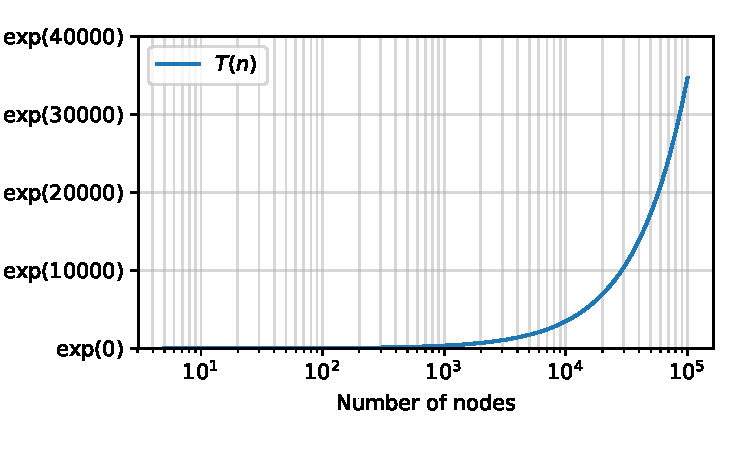
\includegraphics[width=0.7\linewidth]{figs/duda_ch7_prob5}
\caption{Solution to problem 7.5b).}
\label{fig:duda_ch7_prob5}
\end{figure}

# To find the value of $n$ which may be computed in a day, we find $n$ such that
\begin{equation*}
	T(n) = 3600 \cdot 24 \quad \text{   or, alternatively   } \quad \ln T(n) = \ln (3600 \cdot 24).
\end{equation*}
Working in log-space avoids numerical overflow, since $T(n)$ grows very large very quickly.
The answers are:
\begin{alignat*}{2}
	\text{A day: } &  \quad \ln T(n) = \ln (3600 \cdot 24) \quad&\Rightarrow n = 40 \\
	\text{A year: } &  \quad \ln T(n) = \ln (3600 \cdot 24 \cdot 365) \quad&\Rightarrow n = 48 \\
	\text{A century: } &  \quad \ln T(n) = \ln (3600 \cdot 24  \cdot 365 \cdot 100) \quad &\Rightarrow n = 55
\end{alignat*}

\end{easylist}


\subsubsection*{Problem 7.6}
We wish to show that at high temperature, every configuration is equally likely.
The probability that a system is in a configuration of energy $E_\gamma$ is given by Equation (3) in chapter 7 the book, i.e. $P(\gamma) \propto \exp(-E_\gamma / T)$.
As $T$ goes to infinity, we have
\begin{equation*}
	\lim_{T \to \infty} P(\gamma) = 
	\lim_{T \to \infty} \left( e^{-1 / T} \right)^{E_\gamma} = 1^{E_\gamma} = 1,
\end{equation*}
and so the probability of every state $\gamma$ is equally likely. The normalization constant $Z(T)$ makes it a true probability function, i.e. ensures that it sums to unity.




\subsubsection*{Computer exercise 7.2}
A simple implementation of Algorithm 1 in from Chapter 7 is found in the Python file \verb|simulated_annealing.py|.
The answers to sub-problem a) and b) are shown in Figures \ref{fig:ch7_computer_ex2_a} and \ref{fig:ch7_computer_ex2_b} respectively.
A plot showing the average reduction in energy over 500 runs in show in Figure  \ref{fig:ch7_computer_ex2_extra}, and it's interesting to see that the average reduction appears to be exponential.


\begin{figure}[ht!]
\centering
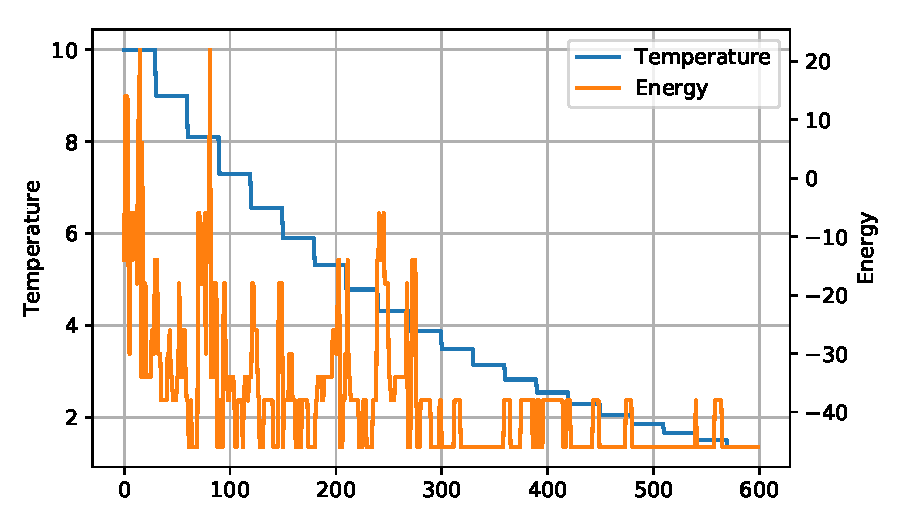
\includegraphics[width=0.7\linewidth]{figs/ch7_computer_ex2_a}
\caption{Simulated annealing with $T(1) = 10$ and $c = 0.9$.
	A total of $20$ main iterations (with fixed temperature), and $5n$ sub iterations (with the same temperature) gives $100 n = 600$ iterations.}
\label{fig:ch7_computer_ex2_a}
\end{figure}

\begin{figure}[ht!]
	\centering
	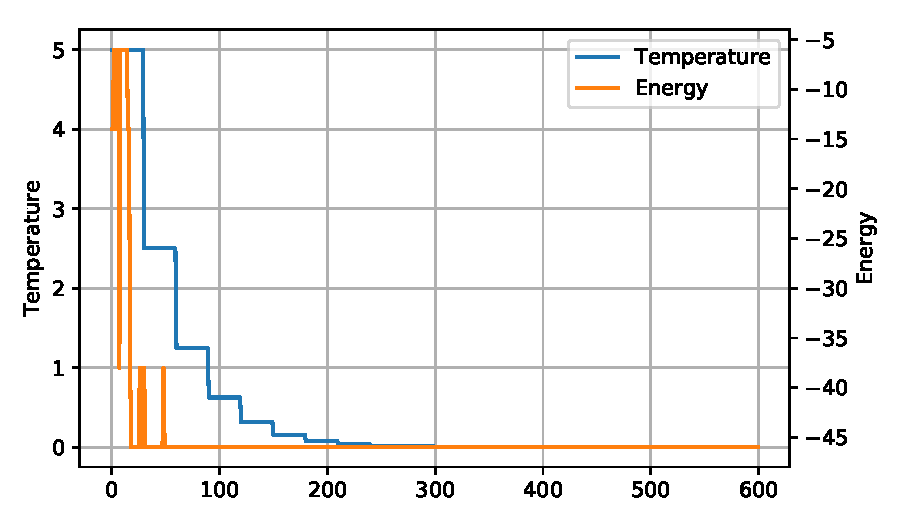
\includegraphics[width=0.7\linewidth]{figs/ch7_computer_ex2_b}
	\caption{Simulated annealing with $T(1) = 5$ and $c = 0.5$.
		A total of $20$ main iterations (with fixed temperature), and $5n$ sub iterations (with the same temperature) gives $100 n = 600$ iterations.}
	\label{fig:ch7_computer_ex2_b}
\end{figure}

\begin{figure}[ht!]
	\centering
	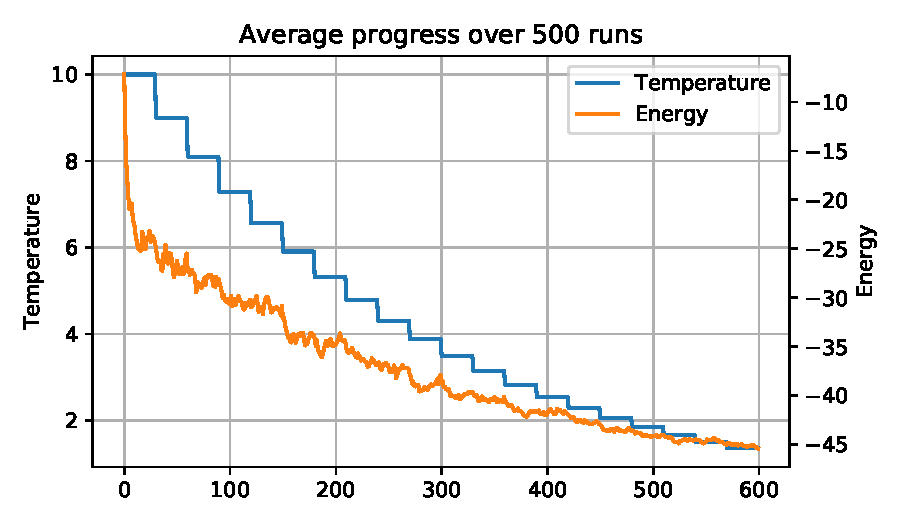
\includegraphics[width=0.7\linewidth]{figs/ch7_computer_ex2_extra}
	\caption{Simulated annealing over 500 runs with $T(1) = 10$ and $c = 0.9$.
		A total of $20$ main iterations (with fixed temperature), and $5n$ sub iterations (with the same temperature) gives $100 n = 600$ iterations.}
	\label{fig:ch7_computer_ex2_extra}
\end{figure}



\clearpage
\subsection{Nonmetric methods}
\subsubsection*{Problem 8.10}
\begin{easylist}[enumerate]
\ListProperties(Space=\listSpace, Space*=\listSpace, Numbers1=l, FinalMark1={)})
# One of the defining properties of an impurity function is that it should be zero when only $\omega_1$ is present, or when only $\omega_2$ is present.
For a polynomial to incorporate this information, it must have two zero points, and therefore it must at least be quadratic.

# The simplest quadratic form of $P(\omega_1)$ obeying the boundary conditions is
\begin{equation*}
	i(P(\omega_1)) \propto P(\omega_1) \left[1 -  P(\omega_1)\right] =  P(\omega_1) P(\omega_2).
\end{equation*}

# Let $X$ be a Bernoulli variable, with $X \in \{0, 1\} = \{\omega_2, \omega_1 \} = C$ and $P(X = 1) = P(\omega_1)$.
In the given problem, we do not know the true probabilities---but they may be estimated from the fractions.
The variance of $X$ is given by
\begin{align*}
	\var \left[ X \right] &= \sum_{w_j \in C} P( \omega_j) \left[ \omega_j - \mu \right]^2 \\
	&= P( \omega_1) \left[ \omega_1 - \mu \right]^2 + P( \omega_2) \left[ \omega_2 - \mu \right]^2 \\
	&= P( \omega_1) \left[ 1 - \mu \right]^2 + \left( 1 - P( \omega_1) \right) \left[ 0 - \mu \right]^2 \\
	&= P( \omega_1) \left[ 1 - P( \omega_1) \right]^2 + \left( 1 - P( \omega_1) \right) P( \omega_1)^2 \\
	&=  \left[ 1 - P( \omega_1) \right] \left[ P( \omega_1) \left(1 - P( \omega_1)\right) + P( \omega_1)^2 \right] \\
	&= \left( 1 - P( \omega_1) \right) P( \omega_1).
\end{align*}
In other words, sample variance is proportional to the impurity estimate defined in subproblem b).
If the variance is high, the data is impure.
\end{easylist}


\subsubsection*{Problem 8.14}
We generalize the problem of a single missing attribute in a single training point to several missing attributes, and to several deficient training points.

In this problem, a pattern $\vect{x} = (x_1, x_2, \dots ,x_d)$ with $d$ attributes can have between $0$ and $d-1$ missing attributes.
Furthermore, the data set $\D = \{\vect{x}_1, \vect{x}_2, \dots, \vect{x}_n \}$ may have many training points with missing attributes.
The data might look something like what is presented in Table \ref{table:problem8_14} on page \pageref{table:problem8_14}.

\begin{table}[hb!]
	\centering
	\caption{Example of what data for problem 8.14 might look like.}
	\begin{tabular}{@{}llll@{}} \toprule
		$x_1$	& $x_2$ & $\dots$ & $x_d$  \\ \midrule
		0 & $\emptyset$ & $\dots$ & 1 \\
		$\emptyset$ & $\emptyset$ & $\dots$ &  1 \\
		1 & $\emptyset$ & $\dots$ & $\emptyset$ \\
		$\vdots$ & $\vdots$ & $\vdots$ & $\vdots$ \\
		0 & $\emptyset$ & $\dots$ & 1 \\ \bottomrule
	\end{tabular}
	\label{table:problem8_14}
\end{table}

High level Python-like pseudocode is given below. 
The principal difference between the code below and the code for the same problem without missing attributes, is that there might now be $n - m_i - 1$ possible splits, where $m_i$ are the number of data points missing from attribute $i$.
This is in contrast to the original algorithm, where there are in general $n-1$ possible splits for every attribute $i$.
\begin{Verbatim}
for attribute=1 to d do:
  attribute_data = data[attribute, :]
  num_missing = count_missing(attribute_data)
  
  best_split = None
  maximal_impurity_gain = -inf
  
  for possible_split=1 to (n - 1 - num_missing) do:
    impurity_gain = compute_gain(attribute_data, possible_split)
    
    if impurity_gain > maximal_impurity_gain:
	  best_split = (attribute, possible_split)
	  maximal_impurity_gain = impurity_gain
	  
  split_along_maximal_impurity_gain(best_split)
\end{Verbatim}


\subsubsection*{Problem 8.16}
\begin{easylist}[enumerate]
	\ListProperties(Space=\listSpace, Space*=\listSpace, Numbers1=l, Numbers2=r, FinalMark1={)})
	# The following tree was constructed by hand. Recall that \textsc{yes} is to the left, and \textsc{no} is to the right.
	The notation $\omega_{ij}$ signifies a pattern $j$ from category $i$.
	\begin{equation*}
	\begin{tikzcd}
	 & x_2 =0 \arrow{dr}{\text{no}} \arrow{dl}{\text{yes}} &  &  \\
	\{\omega_{12}, \omega_{13}, \omega_{14}\} &  & x_3 = 0 \arrow{dr}{\text{no}} \arrow{dl}{\text{yes}} &  \\
	 & \{\omega_{11}, \omega_{21}\} &  & \{\omega_{22}, \omega_{23}, \omega_{24}\} 
	\end{tikzcd}
	\end{equation*}
	The leftmost leaf node assigns to $\omega_1$ with probability 1, the middle leaf node assigns to either $\omega_1$ or $\omega_2$ with probability 0.5, and the rightmost node assigns to $\omega_2$ with probability 1.
	
	# The resulting tree would be identical to the one given in subproblem a), but the assignment from the middle node should be $\omega_1$ with probability $2/3$.
	
\end{easylist}



\subsubsection*{Problem 8.18}
We will consider every alignment of $\vect{x}$ and \emph{text}.
For each of these alignments, there will between $1$ and $m$ comparisons before termination, depending on whether matches are found or not.
There is a probability $d^{-1}$ of a match for each comparison.
We will see that expected number of comparisons may be expressed as a \emph{arithmetico-geometric} sum, i.e. a sum of terms which are the product of an arithmetic and geometric sum.

We start out by observing that there are $n - m + 1$ alignments of $\vect{x}$ and \emph{text}.
For every alignment, at most $m$ characters must be compared.
Let $1 \leq  \ell \leq m$ be the number of comparisons made before the loop terminates.
The loop terminates when a comparison yields no match.
Fixing $\vect{x}$ and considering every character of \emph{text} to be randomly drawn from an alphabet $\mathcal{A}$ of $d$ characters, there is a probability of $d^{-1}$ of a match in each comparison.

Let us now study $P(\ell)$, the probability of $\ell$ comparisons before termination of the loop. 
For instance $P(\ell) = 1 - 1/d$, since it represents the probability of one comparison before exiting the loop, and this happens if there is no match on the first comparison.
More generally, we observe that
\begin{alignat*}{2}
	P(\ell = 1) &= 1 - \frac{1}{d} &\qquad (\text{no match on the first}) \\
	P(\ell = 2) &= \left(1 - \frac{1}{d}\right) \frac{1}{d} &\qquad (\text{match, then no match}) \\
	P(\ell = 2) &= \left(1 - \frac{1}{d}\right) \frac{1}{d^2} &\qquad (\text{match, match, then no match}) \\
	\vdots \quad &= \quad \vdots &  \\
	P(\ell = m) &= \left(1 - \frac{1}{d}\right) \frac{1}{d^{m-1}} + \frac{1}{d^m} &\qquad (\text{no match on final, or match on final}) \\
\end{alignat*}
We now take the expected value of $\ell$ to obtain the expected number of comparisons, and introduce a variable $r := 1/d$ for notational convenience.
\begin{align*}
	\E \left[ \ell \right] = \sum_{k=1}^{m} P(\ell = k) \, k
	& = \left(1 - \frac{1}{d}\right) \left( 1 + \frac{2}{d} + \frac{3}{d^2} + \dots + \frac{m}{d^{m-1}} \right) + \frac{m}{d^m} \\
	& = \left(1 - r\right) \left( 1 + 2r + 3r^2 + \dots + m r^{m-1} \right) + m r^m 
\end{align*}
The sum in the second parenthesis in the first term is a arithmetico-geometric series.
Using the summation formula\footnote{See Wikipedia for the summation formula of a arithmetico-geometric series.} we obtain
\begin{align*}
\E \left[ \ell \right] = \sum_{k=1}^{m} P(\ell = k) \, k
& =\left(1 - r\right) \left( 1 + 2r + 3r^2 + \dots + m r^{m-1} \right) + m r^m \\
&=\left(1 - r\right) \left( 
\frac{1 - (1-m) r^m}{1 - r}
+ 
\frac{r(1 - r^m)}{(1 - r)^2}
 \right) + m r^m \\
 &=
 \frac{(1-r) - (1-r)(1+m)r^m + r(1-r^m) + (1-r)mr^m}{1-r}.
\end{align*}
After some algebraic operations on this final fraction, we obtain the desired result 
\begin{equation*}
	\E \left[ \ell \right] = \sum_{k=1}^{m} P(\ell = k) \, k = \frac{1 - r^m}{1 - r} = \frac{1 - d^{-m}}{1 - d^{-1}}.
\end{equation*}
The problem is solved, since the expected number of comparisons is 
\begin{equation*}
	\text{alignments} \times \text{comparisons} = (n - m + 1) \times \frac{1 - d^{-m}}{1 - d^{-1}} .
\end{equation*}
The inequality $(1 - d^{-m})/(1 - d^{-1}) \leq 2$ presented in the problem description stems from the fact that the fraction is the sum of a geometric series
\begin{equation*}
	\frac{1 - d^{-m}}{1 - d^{-1}} = 1 + \frac{1}{d} + \frac{1}{d^2}  + \dots + \frac{1}{d^{m-1}}.
\end{equation*}
When $d=2$ above, the sum equals $2$. 
Clearly, when $d > 2$ the terms become smaller, and the sum must therefore be $< 2$.
Therefore, as long as $d \geq 2$, the sum is $\leq 2$.
This proves the inequality when $d \geq 2$, which is a reasonable assumption considering the problem.


\subsubsection*{Problem 8.22}
\textbf{A naive algorithm} which loops through the alphabet (of size $d$) for every letter in $\vect{x}$ (of size $m$) would give an $O(dm)$ algorithm.
This is not very efficient, and faster algorithms may easily be constructed.

We can construct a \textbf{better algorithm} with runtime $O(d + m)$ as follows.
\begin{verbatim}
1. Construct an empty lookup table for every character in the alphabet
2. For every character and position in x, overwrite the lookup table
\end{verbatim}
Below is actual Python code implementing the pseudocode above.
\begin{Verbatim}
def last_occurence(alphabet, word):
  """
  Returns a mapping F[char] -> last occurrence in word.
  """
  mapping = {i:-1 for i in alphabet}  # This is O(d)

  for index, char in enumerate(word):  # This is O(m)
    mapping[char] = index

  return mapping
\end{Verbatim}
It's possible to make the algorithm closer to $O(\min(m, d))$, if we know the values of $m$ and $d$ before the algorithm starts.
If $d\gg m$ or $m \gg d$, such an algorithm can avoid looping over the longest string, but we will not pursue this any further in this problem.

We are now in a position to answer the questions posed in the problem.
\begin{easylist}[enumerate]
	\ListProperties(Space=\listSpace, Space*=\listSpace, Numbers1=l, FinalMark1={)})
	# The time complexity of the algorithm is $O(m + d)$.
	# The space complexity is $O(d)$ in the algorithm above. We can avoid storing the empty matches (for instance by using the \texttt{collections.defaultdict} data structure in Python) and get the storage down to $O( \text{unique\_chars}(m))$.
	# Running the algorithm above requires $d + m$ operations, so that $\vect{x}=$ ``\texttt{bonbon}'' yields $26 + 6$ operations.
	Since $m < d$ here, we can use a \texttt{collections.defaultdict} data structure in Python and bring it down to $m = 6$ operations.
\end{easylist}
Below is a print showing that \texttt{collections.defaultdict} indeed leads to faster runtime in practice.
The \texttt{collections.defaultdict} data structure is a dictionary (hash-table) which calls a \emph{default factory function} is a value of a given key is not found.
\begin{Verbatim}
  %timeit last_occurence(alphabet, word)
    2.32 microseconds +/- 42 ns per loop
  %timeit last_occurence_defaultdict(alphabet, word)
    1.17 microseconds +/- 3.17 ns per loop
\end{Verbatim}


\subsubsection*{Problem 8.26}
\begin{easylist}[enumerate]
\ListProperties(Space=\listSpace, Space*=\listSpace, Numbers1=l, Numbers2=r, FinalMark1={)})
# The properties of a metric $D(\vect{a}, \vect{b})$ are
(i) Non-negativity; 
(ii) Reflexivity; 
(iii) Symmetry; and 
(iv) Triangle inequality. These properties are listed on page 187 in \cite{duda_pattern_2000}, which corresponds to Section 4.6.1.
In order, we see that
\begin{easylist}
	## Non-negativity is always obeyed, since every cost is positive.
	## Reflexivity is always obeyed, since if $\vect{a} = \vect{b}$ no operation is performed and the total cost of transformation is zero.
	## Symmetry is not always obeyed. A counterexample follows.
	## The triangle inequality is not always obeyed. A counterexample follows.
\end{easylist}

# We provide counterexamples for symmetry and the triangle inequality.

\textbf{Counterexample for symmetry} 
Let $\vect{a} = \mathtt{dog}$ and $\vect{b} = \mathtt{dogs}$.
Define the distance $D(\vect{a}, \vect{b})$ as the cost of transforming $\vect{a}$ to $\vect{b}$.
Then $D(\vect{a}, \vect{b})$ is the distance of a single insertion to transform $\mathtt{dog} \mapsto \mathtt{dogs}$, while $D(\vect{b}, \vect{a})$ is the distance of a single deletion $\mathtt{dogs} \mapsto \mathtt{dog}$.
If the cost of insertion and deletion differ, then $D(\vect{a}, \vect{b}) \neq D(\vect{b}, \vect{a})$.
This provides a counterexample of the symmetry property of a metric when the costs of operations may be different.

\textbf{Counterexample for the triangle inequality} 
Let $\epsilon$ be the empty string.
Consider the transformation shown in the diagram below.
If the cost of substitution is much greater than the cost of deletion and insertion, then $D(\mathtt{a}, \epsilon) + D(\epsilon, \mathtt{b}) \ll D(\mathtt{a}, \mathtt{b})$. 
This provides a counterexample of the triangle inequality of a metric.

\begin{equation*}
\begin{tikzcd}
\mathtt{a} \arrow{rr}{\text{substitution}}
\arrow[swap]{dr}{\text{deletion}} &  & \mathtt{b} \\
 & \epsilon \arrow[swap]{ur}{\text{insertion}}  & 
\end{tikzcd}
\end{equation*}
\end{easylist}




\subsubsection*{Problem 8.31}
\begin{easylist}[enumerate]
	\ListProperties(Space=\listSpace, Space*=\listSpace, Numbers1=l, Numbers2=r, FinalMark1={)})
	# A grammar generating  $\mathcal{L}(G) =
	\{   \mathtt{a}^n \mathtt{b} \mid n \geq 1   \}$ is, for instance, given by
	\begin{gather*}
		\mathcal{A}  = \{a, b\} \qquad \mathcal{S}  = S \qquad
		\mathcal{I}  = \{A\}
		\\
		\mathcal{P}  = \{S \to Ab, A \to a, A \to Aa\}.
	\end{gather*}
	
	# Below is a derivation tree showing how $ab$ and $aaaaab$ are generated.
	\begin{equation*}
	\begin{tikzcd}
	S \arrow{r} & \arrow{r} \arrow{d}  Ab & \arrow{r} \arrow{d} Aab &  \arrow{r} \arrow{d} Aaab & Aaaab \arrow{d} \arrow{r} & Aaaaab \arrow{d} \arrow{r} & \dots  \\
	&  ab & aab & aaab & aaaab & aaaaab & &
	\end{tikzcd}
	\end{equation*}
\end{easylist}


\subsubsection*{Problem 8.32}
\begin{easylist}[enumerate]
	\ListProperties(Space=\listSpace, Space*=\listSpace, Numbers1=l, Numbers2=r, FinalMark1={)})
	# Since $\mathbf{Type } \, 3 \subset \mathbf{Type } \, 2 \subset \mathbf{Type } \, 1$, we check if it's a \textbf{Type} 3 (regular) grammar first.
	It's not a regular grammar, since the rule $B \to aBa$ is not of the form $\alpha \to z \beta$ or of the form $\alpha \to z$.
	It is, however,  a \textbf{Type} 2 (context-free) grammar since every rule is of the form $I \to \gamma$.
	In other words, every rewrite rule is from an intermediate symbol $I$ to a string $\gamma$ made up of intermediate of terminal symbols.
	
	# To see that the grammar generates the language $\mathcal{L}(G) =
	 \{   \mathtt{ca}^n \mathtt{cba}^n \mathtt{b} \mid n \geq 1   \}$, we draw a derivation tree with intermediate states in the first row, and final states in the second row.
	 The rule $B \to cb$ is highlighted in boldface.
	\begin{equation*}
	\begin{tikzcd}
	S \arrow{r} & \arrow{r}  cAb & \arrow{r} \arrow{d} caBab &  \arrow{r} \arrow{d} caaBaab & caaaBaaab \arrow{d} \arrow{r} & \dots  \\
	&   & ca\mathbf{cb}ab & caa\mathbf{cb}aab & caaa\mathbf{cb}aaab & &
	\end{tikzcd}
	\end{equation*}
	Clearly moving down from $caBab$ produces $\{   \mathtt{ca}^n \mathtt{cba}^n \mathtt{b} \mid n =1   \}$, and moving $\ell$ to the right from $caBab$, and then down, produces $\{   \mathtt{ca}^n \mathtt{cba}^n \mathtt{b} \mid n = \ell + 1   \}$.
	
	# See the solution to subproblem b) above for derivation trees.
\end{easylist}




\clearpage
\subsection{Algorithm-independent machine learning}

\subsubsection*{Problem 9.9}
\begin{easylist}[enumerate]
\ListProperties(Space=\listSpace, Space*=\listSpace, Numbers1=l, FinalMark1={)})
# The binomial theorem is
\begin{equation*}
	(x + y)^n = \sum_{r=0}^{n} \binom{n}{r} x^r y^{n-r}
	= x^n + n x^{n-1}y + \dots + n xy^{n-1} + y^n,
\end{equation*}
and when we substitute $x=y=1$ the result immediately follows, since
\begin{equation*}
2^n = (1 + 1)^n = \sum_{r=0}^{n} \binom{n}{r} 1^r 1^{n-r} 
= \sum_{r=0}^{n} \binom{n}{r}.
\end{equation*}

# The \emph{base case} of the inductive argument is straightforward, we have
\begin{equation*}
	K(1) = \sum_{r=0}^{1} \binom{1}{r} = \binom{1}{0} + \binom{1}{1} = 1 + 1 = 2.
\end{equation*}

To solve the problem of the \emph{inductive step}, we will need to use following three observations:
\begin{equation*}
	\binom{n}{r} = \binom{n-1}{r} + \binom{n-1}{r-1}
	\qquad 
	\binom{n}{n} = 1
	\qquad 
	\binom{n}{0} = 1
\end{equation*}
The first one might be familiar from the construction of Pascals triangle, and the final two are easily derived when writing out $\binom{n}{r} := n! / (n-r)! r!$.

The strategy is to write out $K(n+1)$, strip off the first and last term in the sum, apply the first identity above, and then collect terms to obtain $K(n)$ twice.
We proceed:
\begin{align*}
	K(n+1) &= \sum_{r=0}^{n+1} \binom{n+1}{r} \\
	&= \binom{n+1}{0} + \sum_{r=1}^{n} \left[\binom{n+1}{r}\right] + \binom{n+1}{n+1} \\
	&= 1 + \sum_{r=1}^{n} \left[\binom{n}{r} + \binom{n}{r-1}\right] + 1 \\
	&= \left[1 + \sum_{r=1}^{n} \binom{n}{r}\right] +\left[ \sum_{r=1}^{n} \binom{n}{r-1} + 1\right] \\
	&= \sum_{r=0}^{n} \binom{n}{r} + \sum_{r=0}^{n} \binom{n}{r} =
	K(n) + K(n) = 2K(n)
\end{align*}
If $K(n+1) = 2K(n)$ and $K(1) = 2$, then $K(n) = 2^n$ for all $n$, which is what we wanted to prove.
\end{easylist}



\subsubsection*{Problem 9.13}
\begin{easylist}[enumerate]
\ListProperties(Space=\listSpace, Space*=\listSpace, Numbers1=l, FinalMark1={)})
# The $n$ length string \texttt{010110111011110...} has the pattern \texttt{01-011-0111-01111}, which may be generated using a for-loop.
To generate $n$ bits, we need a counter $c$ keeping track of the number of \texttt{1}s. 
For instance, to generate the $2 + 3 + 4 + 5 = 14$ bit string \texttt{01-011-0111-01111} the counter must go to $4$.
Similarly, to generate the $2 + 3 + 4 + 5  + 6= 20$ bit string \texttt{01-011-0111-01111-011111} the counter must go to $5$.

More generally, to generate $n$ the counter $c$ must go to approximately 
\begin{equation*}
	1 + 2 + 3 + \dots + c = n = \frac{c(c-1)}{2}.
\end{equation*}
Therefore, we need a counter going to $\sim \sqrt{n}$ to generate a $n$ bit string.
Storing the number $c$ requires $\log_2 c$ bits, so the complexity is $O \left( \log_2 \sqrt{n} \right)$.

# We must iterate over $\sim n/2$ zeros, then output a \texttt{1}, then iterate over $\sim n/2$ zeros again.
To do this, we need a counter going to $n/2$, storing this requires $\log_2 (n/2)$ bits, so the Kolmogorov complexity is $O \left( \log_2 n \right)$.

# The complexity is $O(1)$, since there exists programs of finite size which will yield any arbitrarily large number of consecutive digits of $e$.
This is the same reason as why $\pi$ is $O(1)$, as explained in Section 9.2.3 in \cite{duda_pattern_2000}.

# Also constant, for the same reason as the previous sub-problem.

# Assuming a finite size program which generates the digits of $\pi$ one-by-one exists, we use a counter to substitute every 100th digit of $\pi$ in the base-2 number system to a \texttt{1}.
The counter resets after hitting 100, so its storage is constant.
The total complexity is $O(1)$, i.e. constant.

# Same as in the previous question, but storing the counter requires $\log_2 n$ bits.
 Therefore the complexity is $O \left( \log_2 n \right)$.
\end{easylist}


\subsubsection*{Problem 9.18}
We use the relation $\var\left[ X \right] = \E\left[ (X -  \E\left[X \right])^2 \right] = \E \left[X^2\right] + \E \left[X\right]^2$, solve for $\E \left[X^2\right]$ and substitute $X \mapsto g(\vect{x}; \D) -F (\vect{x})$.
Doing this, we observe that
\begin{align*}
	\E \left[X^2\right] 
	&= \E \left[X\right]^2 +  \var\left[ X \right] 
	\\
	\E \left[\left(  g(\vect{x}; \D) -F (\vect{x}) \right)^2\right] 
	&= 
	\underbrace{\E \left[g(\vect{x}; \D) - F (\vect{x}) \right]^2}_{\text{bias}^2} +  
	\underbrace{\var\left[ g(\vect{x}; \D) -F (\vect{x}) \right] }_{\text{variance}}.
\end{align*}
The last term for the variance is not immediately recognizable as the term given in the book, but we note that
\begin{align*}
	\var\left[ g(\vect{x}; \D) -F (\vect{x}) \right]
	& =
	\E \left[ \left( g(\vect{x}; \D) -F (\vect{x}) - \E \left[ g(\vect{x}; \D) -F (\vect{x}) \right] \right)^2 \right] \\
	&= 
	\E \left[ \left( g(\vect{x}; \D)  - \E \left[ g(\vect{x}; \D) \right] \right)^2 \right]
\end{align*}
since $\E \left[ F (\vect{x}) \right] = F (\vect{x})$.
In other words,  $F (\vect{x})$ is the true function and it's expected value is itself.
Combining the results above, we have
\begin{equation*}
	\E \left[\left(  g(\vect{x}; \D) -F (\vect{x}) \right)^2\right] 
	= 
	\underbrace{\E \left[g(\vect{x}; \D) - F (\vect{x}) \right]^2}_{\text{bias}^2} +  
	\underbrace{\E \left[ \left( g(\vect{x}; \D)  - \E \left[ g(\vect{x}; \D) \right] \right)^2 \right]}_{\text{variance}}
\end{equation*}
as stated.

The \emph{bias} can be negative, for instance if the estimate is much lower in value than the true function. 
However, the \emph{squared bias} is always non-negative.
The \emph{variance} is non-negative, since
\begin{equation*}
	\var\left[ X \right] = \E\left[ (X -  \E\left[X \right])^2 \right]
\end{equation*}
by definition, and the squared term is always non-negative.




\subsubsection*{Problem 9.23}
We prove that the average of the leave-one-out means $\mu_{(\cdot)}$ is equivalent to the sample mean $\hat{\mu} = \bar{x}$ by substitution.
Starting with the definition of $\mu_{(\cdot)}$, we have
\begin{align*}
	\mu_{(\cdot)} &= \frac{1}{n} \sum_{i=1}^{n} \mu_{(i)}
	= \frac{1}{n} \sum_{i=1}^{n} \left[  \frac{n \bar{x} - x_i}{n-1} \right]
	= \frac{1}{n(n-1)} \sum_{i=1}^{n} \left[  n \bar{x} - x_i \right] \\
	&= \frac{1}{n(n-1)} \left[ n^2 \bar{x} - n \bar{x} \right]
	=
	\frac{n\bar{x} - \bar{x}}{n-1} = \bar{x} = \frac{1}{n} \sum_{i=1}^{n} x_i.
\end{align*}

\subsubsection*{Problem 9.26}
There is an error in Equation (23) in chapter 9 in the book.
The equation cannot possibly measure the variance (the uncertainty) of a mean value.
To see this, consider two data sets and the results of applying Equation (23):
\begin{align*}
	\D_1 = \left\{0,0,1, 1\right\}  & \mapsto_{(23)} 0.75 \\ 
	\D_2 = \left\{0,0,0,0,0,0,0,0,0,0,1,1,1,1,1,1,1,1,1,1\right\}  & \mapsto_{(23)} 4.75
\end{align*}
Clearly we are more certain about the mean of $\D_2$ than $\D_1$, but this is not reflected in the estimate of the variance of the mean.
Equation (23) should be
\begin{equation*}
\hat{\sigma}^2 = \frac{1}{n (n-1)} \sum_{i=1}^{n} \left( x_i - \hat{\mu} \right)^2,
\end{equation*}
since
\begin{equation*}
	\var \left[ \bar{X} \right] = \var \left[ \frac{1}{n} \sum_{i=1}^{n}  X_i \right]
	= \frac{1}{n^2} \sum_{i=1}^{n} \var \left[    X_i \right]
	= \frac{1}{n} \var \left[    X \right]
	= \frac{1}{n (n-1)} \sum_{i=1}^{n} \left( x_i - \hat{\mu} \right)^2.
\end{equation*}
Then $\D_1  \mapsto 0.08333$ and $\D_2  \mapsto 0.0131578$, which is more in line with what we'd expect---more observations reduce the uncertainty.

Onto the problem at hand: to show that Equation (26) reduces to the above, we write
\begin{equation*}
	\mu_{(i)} - \mu_{(\cdot)} = \left[  \frac{n \bar{x} - x_i}{n-1} \right] - \bar{x} = \frac{\bar{x} - x_i}{n-1}.
\end{equation*}
Squaring this and pulling $(n-1)^2$ out of the sum yields the relationship
\begin{equation*}
	\var \left[ \hat{\mu} \right] = \frac{n-1}{n} 
	\sum_{i=1}^{n} \left( \mu_{(i)} - \mu_{(\cdot)} \right)^2
	= \frac{n-1}{n} 
	\sum_{i=1}^{n} \left( \frac{\bar{x} - x_i}{n-1} \right)^2
	= \frac{1}{n (b-1)} 
	\sum_{i=1}^{n} \left(\bar{x} - x_i \right)^2
\end{equation*}
as desired.


\subsubsection*{Problem 9.34}
See Figure \ref{fig:duda_ch9_prob34} on page \pageref{fig:duda_ch9_prob34} for a plot accompanying this solution.
\begin{easylist}[enumerate]
	\ListProperties(Space=\listSpace, Space*=\listSpace, Numbers1=l, FinalMark1={)})
	# We find the maximum likelihood estimate for $x_\ell$ and $x_u$ to be
	\begin{equation*}
		\hat{x}_\ell = \min \D = 0.2 \qquad 
		\hat{x}_u = \max \D = 0.9.
	\end{equation*}
	Noe that these maximum likelihood estimates are biased.
	The value of $\hat{x}_\ell$ will be greater than the true value of $x_\ell$, and the value of $\hat{x}_u$ will be smaller than the true value of $x_u$.
	The unbiased estimates are
	\begin{align*}
		\hat{x}_u &= \min \D + \frac{n}{n-1} \left( \max \D - \min \D \right) \\
		\hat{x}_\ell &= \min \D - \frac{1}{n-1} \left( \max \D - \min \D \right)
	\end{align*}
	
	# The estimates are $\hat{\mu} = 0.514$ and $\hat{\sigma} = 0.223$, and the maximum likelihood estimate of $\sigma$ is biased.
	
	# The problem states that there is no prior reason to assume one model over the other, so $P(h_1) = P(h_2) = 0.5$.
	We will not make any assumptions on the range of parameter values in $\vect{\theta}$, so the term $p(\hat{\vect{\theta}} \mid h_i) \Delta \vect{\theta}$ in Equation (42) in the book is set to 1.
	What's left is to evaluate $\ln P(\D \mid \hat{\vect{\theta}}, h_i)$, which becomes
	\begin{align*}
		\ln P(\D \mid \hat{\vect{\theta}}, h_1) &= 
		\sum_{i=1}^{n} \ln p(x_i \mid  \hat{x}_\ell = 0.2, \hat{x}_u = 0.9) = \left(\frac{1}{0.7}\right)^{7} \approx 2.497 \\
		\ln P(\D \mid \hat{\vect{\theta}}, h_2) &= 
		\sum_{i=1}^{n} \ln p(x_i \mid  \hat{\mu} = 0.514, \hat{\sigma} = 0.223) \approx 0.567
	\end{align*}
	We decide on model $h_1$, since it's associated with much greater likelihood.
\end{easylist}
	
\begin{figure}[ht!]
\centering
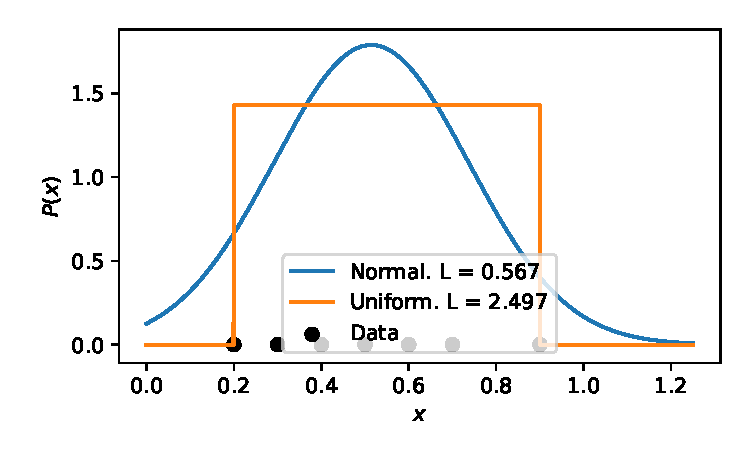
\includegraphics[width=0.65\linewidth]{figs/duda_ch9_prob34}
\caption{Plot of data and models for Problem 9.34.}
\label{fig:duda_ch9_prob34}
\end{figure}


\subsubsection*{Problem 9.37}
The plot for this problem found in Figure \ref{fig:duda_ch9_prob37_k50} on page \pageref{fig:duda_ch9_prob37_k50}.
To create the plot, and outer loop for values of $n$ was used.
For each value of $n$, a true value of $p$ was set.
Then given $(n, p)$, a range of values for a 95 \% confidence interval was computed.
These values were stored and plotted.
Notice that the graph is somewhat jagged when $n$ is small because of the discrete structure of the problem.
	
\begin{figure}[ht!]
\centering
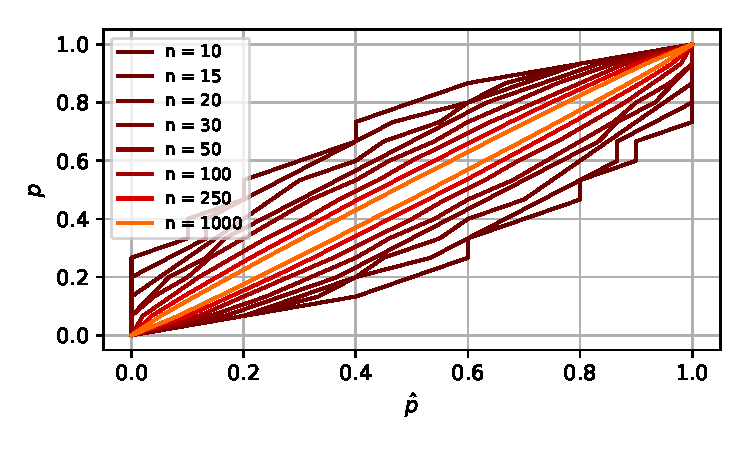
\includegraphics[width=0.7\linewidth]{figs/duda_ch9_prob37_k15}
\caption{Plot associated with Problem 9.37.}
\label{fig:duda_ch9_prob37_k50}
\end{figure}

\subsubsection*{Problem 9.40}
We wish to maximize the likelihood $P(\D \mid \theta) = P(k \mid p)$, where the model is given by the binomial distribution 
$P(k \mid p) = \binom{n}{k} p^k (1-p)^{n-k}$.
The log-likelihood becomes
\begin{equation*}
	\ln P(k \mid p) = \ln \binom{n}{k} + k \ln p + (n-k) \ln (1-p),
\end{equation*}
and differentiating with respect to $p$ and setting this to zero yields
\begin{equation*}
\frac{\partial \ln P(k \mid p)}{\partial p} = \frac{k}{p} + \frac{n-k}{p-1} = 0.
\end{equation*}
The maximum likelihood is the $\hat{p}$ such that the above expression is zero, and solving for $p$ yields $\hat{p} = k / n$ as stated in the problem text.


\clearpage
\subsection{Unsupervised learning and clustering}


\subsubsection*{Problem 10.7}
The log-likelihood of a mixture is given by the expression
\begin{equation*}
	\ell(\alpha) = \sum_{k=1}^{n} \ln p \left( \vect{x}_k \mid \alpha \right)
	= \sum_{k=1}^{n} \ln  \left( 
	\sum_{j=1}^{c} p \left( \vect{x}_k \mid \omega_j,  \alpha \right) P(\omega_j)
	 \right).
\end{equation*}
We'll use the first expression above, differentiate with respect to the parameter $\alpha$, and then expand the sum and differentiate through it with respect to $\alpha$.

Executing the plan outlined above, we observe that
\begin{align*}
	\frac{\partial \ell(\alpha)}{ \partial \alpha}
	&= \sum_{k=1}^{n} \frac{1}{p \left( \vect{x}_k \mid \alpha \right)}
	\frac{\partial}{\partial \alpha}
	 p \left( \vect{x}_k \mid \alpha \right) 	\\
	&= \sum_{k=1}^{n} \frac{1}{p \left( \vect{x}_k \mid \alpha \right)}
	\frac{\partial}{\partial \alpha}
	\left( \sum_{j=1}^{c} p \left( \vect{x}_k \mid \omega_j,  \alpha \right) P(\omega_j) \right) \tag{by definition}	
	\\
	&= \sum_{k=1}^{n} \frac{1}{p \left( \vect{x}_k \mid \alpha \right)}
	 \sum_{j=1}^{c} P(\omega_j) \frac{\partial p \left( \vect{x}_k \mid \omega_j,  \alpha \right)}{\partial \alpha} 
	 \\
	 &= \sum_{k=1}^{n} \sum_{j=1}^{c} \frac{P(\omega_j)}{p \left( \vect{x}_k \mid \alpha \right)}
	   \frac{\partial p \left( \vect{x}_k \mid \omega_j,  \alpha \right)}{\partial \alpha} . \tag{constant into sum}
\end{align*}
Since $(\ln x)' = x' / x$ by the chain rule of calculus, the equation $x' = x (\ln x)'$ holds too.
Using this on the last factor, we observe that 
\begin{equation*}
	\sum_{k=1}^{n} \sum_{j=1}^{c} \frac{P(\omega_j)}{p \left( \vect{x}_k \mid \alpha \right)}
	\frac{\partial p \left( \vect{x}_k \mid \omega_j,  \alpha \right)}{\partial \alpha}
	=
	\sum_{k=1}^{n} \sum_{j=1}^{c} \frac{P(\omega_j)}{p \left( \vect{x}_k \mid \alpha \right)} 
	p \left( \vect{x}_k \mid \omega_j,  \alpha \right)
	\frac{\partial \ln p \left( \vect{x}_k \mid \omega_j,  \alpha \right)}{\partial \alpha}.
\end{equation*}
As stated in the problem text, the first two factors may be simplified using Bayes theorem, since
\begin{equation*}
	P( \omega_j \mid \vect{x}_k, \alpha) 
	= 
	\frac{p(\vect{x}_k \mid  \omega_j, \alpha) P(\omega_j \mid \alpha)}{p( \vect{x}_k,\mid \alpha)}
	= 
	\frac{p(\vect{x}_k \mid  \omega_j, \alpha) P(\omega_j)}{p( \vect{x}_k,\mid \alpha)}
\end{equation*}
when $\omega_j$ is independent of $\alpha$, i.e. $P(\omega_j \mid \alpha) = P(\omega_j )$.
We have completed the problem, since applying the simplification due to Bayes theorem yields the desired result.


\subsubsection*{Problem 10.11}
\begin{easylist}[enumerate]
\ListProperties(Space=\listSpace, Space*=\listSpace, Numbers1=l, FinalMark1={)})
# Solving this problem requires knowledge of matrix calculus.
We will differentiate the second term, and then the first term, and finally combine the results.
The reason we start with the second term is that it is easier.

\textbf{Second term}
Let's start by differentiating $\vect{x}^T \vect{A} \vect{x}$ with respect to an element $A_{ij}$.
This is functionally equivalent to the second term in the problem statement, and solving this solves the original problem.
If $\vect{A}$ is symmetric, then
\begin{equation*}
	\frac{\partial \vect{x}^T \vect{A} \vect{x}}{\partial A_{ij}}
	=
	\frac{\partial \sum_i \sum_j x_i A_{ij} x_j}{\partial A_{ij}}
	=
	\begin{rcases}
		\begin{dcases}
		x_i x_j & \text{ if } i = j \\
		2x_i x_j & \text{ if } i \neq j
		\end{dcases}
	\end{rcases}
	= \left(2 - \delta_{ij}\right) x_i x_j.
\end{equation*}

\textbf{First term}
Let's now consider differentiating $f(\vect{A}) = \ln \left( \det \vect{A} \right)$ with respect to an element $A_{ij}$.
This is functionally equivalent to the first term in the problem statement.
We'll make use of Jacobi's formula\footnote{See Wikipedia for details: \url{https://en.wikipedia.org/wiki/Jacobi's_formula}}, which is given by
\begin{equation*}
	\frac{d}{dt} \det \vect{A}(t) = \operatorname{tr} \left (\operatorname{adj}(\vect{A}(t)) \, \frac{d\vect{A}(t)}{dt}\right ),
\end{equation*}
where $\operatorname{tr}(\vect{A})$ is the trace of $\vect{A}$, and $\operatorname{adj}(\vect{A})$ is the adjugate of $\vect{A}$.

We differentiate using the chain rule and apply Jacobi's formula to obtain
\begin{equation*}
	\frac{\partial \ln \left( \det \vect{A} \right)}{\partial A_{ij}}
	=
	\frac{1}{\det \vect{A}}
	\frac{\partial \det \vect{A} }{\partial A_{ij}}
	=
	\frac{1}{\det \vect{A}}
	\operatorname{tr} \left(  \operatorname{adj}(\vect{A}) \, \frac{\partial \vect{A}}{\partial A_{ij}} \right).
\end{equation*}
Now comes the part where we consider the diagonal elements $i=j$ and off-diagonal elements $i \neq j$ separately.
We carry out the differentiation $d\vect{A} / \partial A_{ij}$ and obtain
\begin{equation*}
\frac{1}{\det \vect{A}}
\operatorname{tr} \left(  \operatorname{adj}(\vect{A}) \, \frac{\partial \vect{A}}{\partial A_{ij}} \right)
=
\begin{rcases}
\begin{dcases}
\frac{1}{\det \vect{A}}
\operatorname{tr} \left(  \operatorname{adj}(\vect{A}) \, \left[  \vect{E}_{ii} \right] \right) & \text{ if } i = j \\
\frac{1}{\det \vect{A}}
\operatorname{tr} \left(  \operatorname{adj}(\vect{A}) \, \left[  \vect{E}_{ij} + \vect{E}_{ji} \right] \right) & \text{ if } i \neq j
\end{dcases}
\end{rcases},
\end{equation*}
where by $\vect{E}_{ij}$ we mean a matrix of zeros everywhere except in the $ij$th position.
We do not show it here, but by the definition of $\vect{E}_{ij}$ and the trace, it should not be too hard to see that $\operatorname{tr} \left(  \vect{A} \,  \vect{E}_{ij}  \right) = A_{ji}$.
Using the above in combination with the fact that $\operatorname{adj}(\vect{A})_{ji} / \det (\vect{A}) = \vect{A}^{-1}_{ji}$ and the fact that the inverse of a symmetric matrix is symmetric, we observe that the above expression may be written using the Kroneker delta symbol $\delta_{ij}$ as
\begin{equation*}
\begin{rcases}
\begin{dcases}
\frac{\operatorname{adj}(\vect{A})_{ii}}{\det \vect{A}}
    & \text{ if } i = j \\
\frac{\operatorname{adj}(\vect{A})_{ji}}{\det \vect{A}}
 +
 \frac{\operatorname{adj}(\vect{A})_{ij}}{\det \vect{A}}  & \text{ if } i \neq j
\end{dcases}
\end{rcases}
=
\begin{rcases}
\begin{dcases}
\vect{A}^{-1}_{ii}  & \text{ if } i = j \\
\vect{A}^{-1}_{ji} + \vect{A}^{-1}_{ij}   & \text{ if } i \neq j
\end{dcases}
\end{rcases}
=
(2 - \delta_{ij}) \vect{A}^{-1}_{ij}.
\end{equation*}
\textbf{Putting it all together}
We have established that if $\vect{A}$ is a symmetric matrix, then
\begin{equation*}
	\frac{\partial \vect{x}^T \vect{A} \vect{x}}{\partial A_{ij}} 
	= 
	\left(2 - \delta_{ij}\right) x_i x_j
	\quad \text{and} \quad
	\frac{\partial \ln \left( \det \vect{A} \right)}{\partial A_{ij}} 
	=
	(2 - \delta_{ij}) \vect{A}^{-1}_{ij}.
\end{equation*}

Applying the two results above to the problem at hand yields
\begin{align*}
	\frac{\partial }{\partial \sigma^{pq}(i)} \left( \ln p \left( \vect{x}_k \mid \omega_i , \vect{\theta}_i \right) \right)
	& =
	\frac{\partial }{\partial \sigma^{pq}(i)} \left(
	\ln \frac{\abs{\vect{\Sigma}_i^{-1}}^{1/2}}{(2 \pi)^{d/2}}
	 - \frac{1}{2}
	 \left( \vect{x}_k - \vect{\mu}_i \right)^T
	 \vect{\Sigma}_i^{-1}
	 \left( \vect{x}_k - \vect{\mu}_i \right)
	 \right) \\
	 & =
	 \frac{\partial }{\partial \sigma^{pq}(i)} \left(
	 \frac{1}{2}\ln \abs{\vect{\Sigma}_i^{-1}}
	 - \frac{1}{2}
	 \left( \vect{x}_k - \vect{\mu}_i \right)^T
	 \vect{\Sigma}_i^{-1}
	 \left( \vect{x}_k - \vect{\mu}_i \right)
	 \right) \\
	 & =
	 \left(1 - \frac{\delta_{pq}}{2} \right) \sigma_{pq}(i)
	 -
	 \left(1 - \frac{\delta_{pq}}{2} \right)
	 \left( x_p(k) - \mu_p(i) \right)
	 \left( x_q(k) - \mu_q(i) \right) \\
	 & =
	 \left(1 - \frac{\delta_{pq}}{2} \right) 
	 \left[
	 \sigma_{pq}(i)
	 - 
	 \left( x_p(k) - \mu_p(i) \right)
	 \left( x_q(k) - \mu_q(i) \right)
	 \right],
\end{align*}
which corresponds with Equation (23) in chapter 10 in the book as expected.

# We will extend the result from the previous sub-problem to every entry in the matrix, then solve for the maximum likelihood estimate for $\vect{\Sigma}$.

If we extend the differentiation formulas from the previous sub-problem to every entry in the matrix, we recognize that
\begin{equation*}
	\frac{\partial \vect{x}^T \vect{A} \vect{x}}{\partial \vect{A}} = \vect{x} \vect{x}^T 
	\qquad \text{and} \qquad
	\frac{\partial \ln (\det \vect{A})}{\partial \vect{A}} =  \vect{A}^{-1}.
\end{equation*}
Applying these equations to the second factor in the solution to problem 7, and ignoring constants, we obtain a result proportional to
\begin{equation*}
	\frac{\partial }{\partial \vect{\Sigma}^{-1}} \left( \ln p \left( \vect{x}_k \mid \omega_i , \vect{\theta}_i \right) \right) = 
	\vect{\Sigma} - \left( \vect{x}_k - \vect{\mu}_i \right)\left( \vect{x}_k - \vect{\mu}_i \right)^T.
\end{equation*}

Our problem becomes that of solving the equation
\begin{align}
	\nonumber &\frac{\partial \ell }{\partial \vect{\Sigma}^{-1}}   =  
	\sum_{k=1}^{n} \sum_{i=1}^{c} P \left( \omega_i \mid \vect{x}_k, \vect{\theta}\right)
	\left[ \vect{\Sigma} - \left( \vect{x}_k - \vect{\mu}_i \right) \left( \vect{x}_k - \vect{\mu}_i \right)^T \right] = \vect{0} \\
	&  \Rightarrow  \,
	\vect{\Sigma} \sum_{k=1}^{n} \sum_{i=1}^{c} P \left( \omega_i \mid \vect{x}_k, \vect{\theta}\right)
	=
	\sum_{k=1}^{n} \sum_{i=1}^{c} P \left( \omega_i \mid \vect{x}_k, \vect{\theta}\right)
	\left[ \vect{x}_k \vect{x}_k^T - 2 \vect{x}_k \vect{\mu}_i^T + \vect{\mu}_i \vect{\mu}_i^T \right] \label{eqn:ch10_prob10}
\end{align}
for $\vect{\Sigma}$.
We will now examine each term of Equation \eqref{eqn:ch10_prob10} separately.

Notice first that the left hand side of equation \eqref{eqn:ch10_prob10} becomes
\begin{equation*}
	\vect{\Sigma}
	\sum_{k=1}^{n} \sum_{i=1}^{c} P 
	\left( \omega_i \mid \vect{x}_k, \vect{\theta}\right) 
	=
	\vect{\Sigma}n \sum_{k=1}^{n} \sum_{i=1}^{c} 
	 p \left(  \vect{x}_k, \omega_i \mid \vect{\theta} \right) 
	 =  \vect{\Sigma} n,
\end{equation*}
where we have made use of Bayes theorem.

Moving to the right hand side of Equation \eqref{eqn:ch10_prob10}, we see that
\begin{equation*}
	\sum_{k=1}^{n} \sum_{i=1}^{c} P \left( \omega_i \mid \vect{x}_k, \vect{\theta}\right)
	\vect{x}_k \vect{x}_k^T
	= 
	\sum_{k=1}^{n}
	\vect{x}_k \vect{x}_k^T,
\end{equation*}
since the sum of the probabilities of each class $c$ must be $1$ for each data point $k$.

The cross term of the right-hand side of Equation \eqref{eqn:ch10_prob10} becomes
\begin{align*}
	- 2 \sum_{k=1}^{n} \sum_{i=1}^{c} P \left( \omega_i \mid \vect{x}_k, \vect{\theta}\right)  \vect{x}_k \vect{\mu}_i^T 
	& =
	- 2  \sum_{k=1}^{c} \left( \sum_{k=1}^{n} P \left( \omega_i \mid \vect{x}_k, \vect{\theta}\right)  \vect{x}_k \right) \vect{\mu}_i^T \\
	& =
	- 2  \sum_{k=1}^{c} \left( \sum_{k=1}^{n} n P \left(  \vect{x}_k \mid \omega_i , \vect{\theta}\right) P(\omega_i \mid \vect{\theta} ) \vect{x}_k \right) \vect{\mu}_i^T \\
	& =
	- 2  \sum_{k=1}^{c} 
	n \vect{\mu}_i P(\omega_i \mid \vect{\theta})
	 \vect{\mu}_i^T
	 = 
	 -2 n \sum_{k=1}^{c} 
	 P(\omega_i \mid \vect{\theta} ) \vect{\mu}_i
	 \vect{\mu}_i^T,
\end{align*}
where the second equality comes from Bayes theorem. 
In the the second to last equality we used $\sum_{k=1}^{n} p(\vect{x}_k \mid \omega_i) \vect{x}_k = \vect{\mu}_i$.

Finally, the rightmost term of the right-hand side of Equation \eqref{eqn:ch10_prob10} becomes
\begin{equation*}
	\sum_{k=1}^{n} \sum_{i=1}^{c} P \left( \omega_i \mid \vect{x}_k, \vect{\theta}\right)
	\vect{\mu}_i \vect{\mu}_i^T
	=
	n \sum_{k=1}^{c} P \left( \omega_i \mid  \vect{\theta}\right)
	\vect{\mu}_i \vect{\mu}_i^T,
\end{equation*}
where again Bayes theorem was used.

Putting all these results back into Equation \eqref{eqn:ch10_prob10}, we finally see that
\begin{equation*}
	\vect{\Sigma} n
	=
	\sum_{k=1}^{n}
	\vect{x}_k \vect{x}_k^T
	-
	n \sum_{k=1}^{c} P \left( \omega_i \mid  \vect{\theta}\right)
	\vect{\mu}_i \vect{\mu}_i^T,
\end{equation*}
and diving through by $n$ gives the desired result.
\end{easylist}

\subsubsection*{Problem 10.12}
\begin{easylist}[enumerate]
	\ListProperties(Space=\listSpace, Space*=\listSpace, Numbers1=l, Numbers2=r, FinalMark1={)})
	# Creating a plot of $p(x \mid \omega_1) = \N(0, 1)$ and $p(x \mid \omega_2) = \N(0, 1/2)$ is illuminating.
	See figure \ref{fig:ch10_prob12} for such a plot, which reveals the significance of $\ln 2$ immediately.
	
		\begin{figure}[ht!]
			\centering
			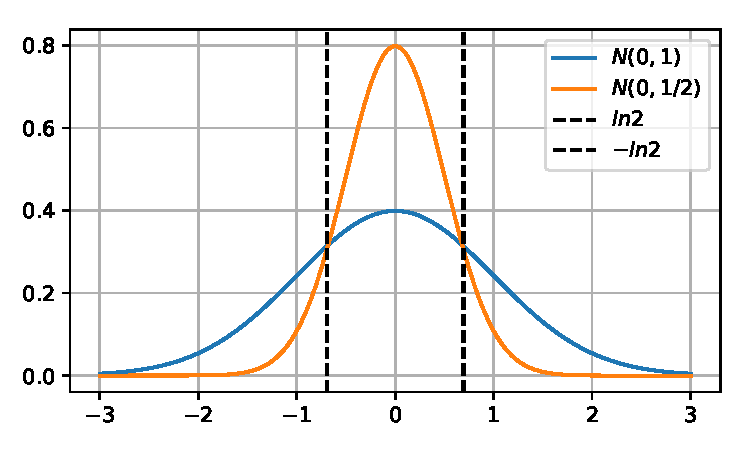
\includegraphics[width=0.6\linewidth]{figs/duda_ch10_prob12.pdf}
			\caption{Plot for problem 12, chapter 10.}
			\label{fig:ch10_prob12}
		\end{figure}
	
	
	The likelihood of the mixture is given by 
	\begin{equation*}
		\ell (x_1 \mid  P(\omega_1)) = p(x_1) = \frac{P(\omega_1)}{\sqrt{2 \pi}} e^{-x_1^2 / 2}
		+
		\frac{(1 - P(\omega_1))}{\sqrt{ \pi}} e^{-x_1^2 },
	\end{equation*}
	and using the logarithm will not aid us in our attempt to maximize this function.
	
	Notice that for a given value of $x_1$, the likelihood is linear in $P(\omega_1)$, since
	\begin{equation*}
		f( P(\omega_1) ) = p(x_1) = P(\omega_1) \, p(x \mid \omega_1) + (1 - P(\omega_1)) \, p(x \mid \omega_1),
	\end{equation*}
	and it's derivative with respect to $P( \omega_1)$ is $f'(P( \omega_1)) = p(x \mid \omega_1) - p(x \mid \omega_2)$.
	Since $0 \leq P(\omega_1) \leq 1$, there are two cases to consider:
	
	\begin{easylist}[enumerate]
		\ListProperties(Space=\listSpace, Space*=\listSpace, Numbers1=l, Numbers2=r, FinalMark1={)})
	## If $f'(P( \omega_1))  > 0$, the likelihood is maximized by the choice $P(\omega_1) = 1$.
	## If $f'(P( \omega_1)) < 0$, the likelihood is maximized by the choice $P(\omega_1) = 0$.
	\end{easylist}
	
	If remains to investigate for which values of $x_1$ the derivative is positive or negative.
	
	We take logarithms to study when $p(x \mid \omega_1) > p(x \mid \omega_2)$ and vice versa, since this determines the sign of the derivative.
	We compare $p(x \mid \omega_1) = \N(0, 1)$ and $p(x \mid \omega_2) = \N(0, 1/2)$ by equating them, taking logarithms and using some algebra:
	\begin{equation*}
	\frac{1}{\sqrt{2}} e^{-x_1^2 / 2}
	=
	e^{-x_1^2 }
	\quad
	\Leftrightarrow
	\quad
	\ln 2 = x_1^2.
	\end{equation*}
	When $x_1^2 < \ln 2$, we find that $e^{-x_1^2 } > \frac{1}{\sqrt{2}} e^{-x_1^2 / 2}$.
	This implies that $p(x \mid \omega_2) > p(x \mid \omega_1)$ and the derivative of the linear function is negative.
	In that case the likelihood is maximized by $P(\omega_1) = 0$, as claimed in the problem.
\end{easylist}
	
	\begin{easylist}[enumerate]
		\ListProperties(Space=\listSpace, Space*=\listSpace, Numbers1=l, Numbers2=r, FinalMark1={)}, Start1=2)

	 # This is simply the reverse case of what we saw in the previous problem. 
	 When $x_1^2 > \ln 2$ we find that $p(x \mid \omega_1) > p(x \mid \omega_2)$ and the derivative is positive.
	 In this case the likelihood is maximized by $P(\omega_1) = 1$.
	 
	 # With two Gaussians having the same mean, but different stanard deviations, the maximum likelihood estimate of $P(\omega_1)$ is either $0$ or $1$ when one data point $x_1$ is seen.
	 The maximum likelihood assigns all weight to the prior corresponding to the class with the largest class-conditional density $p(x \mid \omega_i)$.
	


\end{easylist}

\subsubsection*{Problem 10.14}
From the solution to Problem 6.39, we know that the derivative of $\vect{x}^T \vect{A} \vect{x}$ is $(\vect{A} + \vect{A}^T)\vect{x}$.
This result is also in Appendix A.2 in \cite{duda_pattern_2000}.
To find the minimizer, we differentiate with respect to $\vect{x}$ and find that
\begin{equation*}
	\frac{\partial J(\vect{x})}{\partial \vect{x}} = \sum_{k=1}^{m}
	\left( \vect{\Sigma}^{-1} + \vect{\Sigma}^{-T} \right)
	\left( \vect{x}_k - \vect{x}^* \right) = \vect{0}.
\end{equation*}
Since $\vect{\Sigma}$ may be moved outside of the sum and is non-singular, we require that 
\begin{equation*}
	\sum_{k=1}^{m}
	\left( \vect{x}_k - \vect{x}^* \right) = \vect{0}
	\quad 
	\Leftrightarrow
	\quad 
	\sum_{k=1}^{m}
	 \vect{x}_k  = m \vect{x}^*.
\end{equation*}
Dividing by $m$, we see that $\vect{x}^* = \bar{\vect{x}}$, which is what we wanted to demonstrate.






\subsubsection*{Problem 10.16}
A distance computation between two $d$-dimensional vectors is $O(d)$.
Pseudocode makes the runtime evident, since we essentially only need to count the number of loops.
\begin{Verbatim}
for each iteration (T):
  for each data point (n):
    for each cluster center (c):
      compute distance dist(x_j, mu_i) (d)
\end{Verbatim}
The algorithm has runtime $O(T) \cdot O(n) \cdot O(c) \cdot O(d) = O(Tncd)$ as claimed.



\subsubsection*{Problem 10.21}
Let us assume that $n \geq c$ and that there exists an empty subset.
Then there must exist at least one non-empty subset with more than one sample. 
An example would be $\left\{ \left\{ \vect{x}_1 \right\}, \left\{  \right\}, \left\{ \vect{x}_2, \vect{x}_3 \right\}  \right\}$, where the second subset is empty, and the third subset has more than one sample.
We show that moving a sample from a non-empty subset $\D_\text{non-empty}$ to an empty subset $\D_\text{empty}$ always decreases $J_e$.

The sum-of-squared error over the empty subset $\D_\text{empty}$ does not contribute to $J_e$, since it's only defined over non-empty subsets.
Moving a single sample to $\D_\text{empty}$ contributes 
\begin{equation*}
	\sum_{i=1}^{1} \norm{\vect{x}_i - \vect{m}}^2
	=
	\norm{\vect{x}_1 - \vect{x}}^2
	=
	\norm{\vect{x}_1 - \vect{x}_1}^2
	=
	0
\end{equation*}
to $J_e$, i.e. no contribution at all.
In summary, moving a sample to $\D_\text{empty}$ does not alter the contribution to $J_e$ from the subset $\D_\text{empty}$---it's zero in both cases.

The sum-of-squared error over the non-empty subset $\D_\text{non-empty}$ does contribute to $J_e$.
If $\D_\text{non-empty}$ contains $n$ samples whose mean is $\vect{m}$, the contribution is
\begin{equation*}
\sum_{i=1}^{n} \norm{\vect{x}_i - \vect{m}}^2.
\end{equation*}
Now we remove a sample $\vect{x}_n$ from the subset, to put in the empty subset instead.
As long as the sample $\vect{x}_n$ that we remove is not identical to the mean, we have
\begin{equation*}
	\sum_{i=1}^{n} \norm{\vect{x}_i - \vect{m}}^2
	=
	\sum_{i=1}^{n-1} \norm{\vect{x}_i - \vect{m}}^2
	+ \norm{\vect{x}_n - \vect{m}}^2
	 > 
	 \sum_{i=1}^{n-1} \norm{\vect{x}_i - \vect{m}}^2.
\end{equation*}
In summary, moving a sample from $\D_\text{non-empty}$ \emph{does} alter the contribution to $J_e$ from the subset $\D_\text{non-empty}$---it always decreases.

Combining the statements above reveals that if any empty subset exists, we can always decrease $J_e$.
As a result there are no empty subsets in a partition that minimizes $J_e$.
As an example, the partition $\left\{ \left\{ \vect{x}_1 \right\}, \left\{ \vect{x}_2 \right\}, \left\{ \vect{x}_3 \right\}  \right\}$ will be superior to $\left\{ \left\{ \vect{x}_1 \right\}, \left\{  \right\}, \left\{ \vect{x}_2, \vect{x}_3 \right\}  \right\}$.


\subsubsection*{Problem 10.32}
\begin{easylist}[enumerate]
\ListProperties(Space=\listSpace, Space*=\listSpace, Numbers1=l, FinalMark1={)})
# 
%An example of $\vect{x}$ when $d=3$ is $(1, 1, -1)$.
Let's study the similarity measure under the assumption that $x_i, y_i \in \left\{-1, 1\right\}$.
From the definition, we have that
\begin{equation*}
	s(\vect{x}, \vect{y}) = \frac{\vect{x}^T \vect{y}}{\norm{\vect{x}} \norm{\vect{y}}}
	=
	\frac{\sum_{i=1}^{d} x_i y_i}{\sqrt{d} \sqrt{d}}
	=
	\frac{\sum_{i=1}^{d} \left[ x_i = y_i \right] - \sum_{i=1}^{d} \left[ x_i \neq y_i \right]}{d},
\end{equation*}
where $\left[ \, \cdot \,  \right]$ is the Iverson bracket, returning 1 if the condition in the bracket is true, and 0 if it's false.
An interpretation is therefore
\begin{equation*}
s(\vect{x}, \vect{y}) 
= 
\frac{\sum_{i=1}^{d} \left[ x_i = y_i \right] - \sum_{i=1}^{d} \left[ x_i \neq y_i \right]}{d}
= \frac{\text{num equal} - \text{num different}}{\text{total number}},
\end{equation*}
and we also note that $-1 \leq s(\vect{x}, \vect{y})  \leq 1 $ are tights bounds, realized when every element is different, or element entry is equal, respectively.

# This is shown using algebra.
We solve the problem by realizing that
\begin{align*}
	\norm{\vect{x} - \vect{y}}^2 &= \sum_{i=1}^{d} (x_i - y_i)^2 =
	\sum_{i=1}^{d} x_i^2 
	-
	\sum_{i=1}^{d} 2x_i y_i^2
	+ 
	\sum_{i=1}^{d}  y_i^2 \\
	&= d - 2 \vect{x}^T \vect{y} -d = 2d - 2d \frac{\vect{x}^T \vect{y}}{d}
	= 2s (1 - s(\vect{x}, \vect{y}) ).
\end{align*}
\end{easylist}


\subsubsection*{Problem 10.35}
The smallest increase happens when we merge clusters so that their contribution to $J_e$ increases by as little as possible.
We consider the error from clusters $i$ and $j$ before and after merging, and show that the difference in contribution to $J_e$ is given by the expression in the problem statement.

The contribution before merging is
\begin{equation*}
	\sum_{\vect{x}_i \in \D_i} \norm{\vect{x}_i - \vect{m}_i}^2
	+
	\sum_{\vect{x}_j \in \D_j} \norm{\vect{x}_j - \vect{m}_j}^2.
\end{equation*}
The contribution after merging is
\begin{equation*}
	\sum_{\vect{x}_k \in \D_i \cup \D_j} \norm{\vect{x}_k - \vect{m}}^2
	=
	\sum_{\vect{x}_i \in \D_i} \norm{\vect{x}_i - \vect{m}}^2
	+
	\sum_{\vect{x}_j \in \D_j} \norm{\vect{x}_j - \vect{m}}^2,
\end{equation*}
where $\vect{m} = \vect{m}_i n_i / (n_i +n_j)  + \vect{m}_j n_j / (n_i +n_j) $ is the new mean after merging the clusters.

We now compute the difference, which becomes
\begin{align}
	\nonumber \text{diff} &= \text{after merging} - \text{before merging} \\
	 \nonumber&= \left( \sum_{\vect{x}_i \in \D_i} \norm{\vect{x}_i - \vect{m}}^2
	+
	\sum_{\vect{x}_j \in \D_j} \norm{\vect{x}_j - \vect{m}}^2 \right)
	-
	\left(
	\sum_{\vect{x}_i \in \D_i} \norm{\vect{x}_i - \vect{m}_i}^2
	+
	\sum_{\vect{x}_j \in \D_j} \norm{\vect{x}_j - \vect{m}_j}^2
	\right) \\
	 \label{eq:ch10_problem35} &=
	\sum_{\vect{x}_i \in \D_i}
	\left( \norm{\vect{x}_i - \vect{m}}^2 - \norm{\vect{x}_i - \vect{m}_i}^2 \right)
	+
	\sum_{\vect{x}_j \in \D_j}
	\left( \norm{\vect{x}_j - \vect{m}}^2 - \norm{\vect{x}_j - \vect{m}_j}^2 \right)
\end{align}
To make progress with Equation \eqref{eq:ch10_problem35}, we note that
\begin{align*}
	\sum_{\vect{x}_i \in \D_i} \norm{\vect{x}_i - \vect{m}}^2 - \norm{\vect{x}_i - \vect{m}_i}^2
	&=
	\sum_{\vect{x}_i \in \D_i} \norm{ (\vect{x}_i - \vect{m}_i) - (\vect{m} - \vect{m}_i)}^2 - \norm{\vect{x}_i - \vect{m}_i}^2 \\
	&= \sum_{\vect{x}_i \in \D_i} 
	\norm{ \vect{x}_i - \vect{m}_i}^2 
	+
	\norm{\vect{m} - \vect{m}_i}^2
	- \norm{\vect{x}_i - \vect{m}_i}^2 \\
	&= \sum_{\vect{x}_i \in \D_i} 
	\norm{\vect{m} - \vect{m}_i}^2,
\end{align*}
where we have used the fact that the cross term $\sum_{\vect{x}_j \in \D_j} -2 (\vect{x}_i - \vect{m}_i)^T (\vect{m} - \vect{m}_i)$ is zero. 

Substituting this result back into Equation \eqref{eq:ch10_problem35} we obtain
\begin{align}
\nonumber \text{diff} &= \text{after merging} - \text{before merging} \\
&= 
\nonumber \sum_{\vect{x}_i \in \D_i} 
\norm{\vect{m} - \vect{m}_i}^2 +
\sum_{\vect{x}_j \in \D_j} 
\norm{\vect{m} - \vect{m}_j}^2 \\
&= 
\label{eq:ch10problem35_2} n_i
\norm{\vect{m} - \vect{m}_i}^2 +
n_j
\norm{\vect{m} - \vect{m}_j}^2.
\end{align}

Now we compute the difference 
\begin{equation*}
	\vect{m} - \vect{m}_i =
	 \left( \vect{m}_i \frac{n_i}{n_i + n_j}
	 +
	 \vect{m}_j \frac{n_j}{n_i + n_j}
	  \right)
	  -
	  \vect{m}_i
	  = 
	  \frac{n_j}{n_i + n_j} (\vect{m}_j - \vect{m}_i),
\end{equation*}
and use this result in Equation \eqref{eq:ch10problem35_2} to see that
\begin{align*}
	 \text{diff} &= \text{after merging} - \text{before merging} \\
	&= 
	n_i
	\frac{n_j^2}{(n_i + n_j)^2} \norm{\vect{m}_j - \vect{m}_i}^2
	+
	n_j
	\frac{n_i^2}{(n_i + n_j)^2} \norm{\vect{m}_i - \vect{m}_j}^2 \\
	&=  \frac{n_i n_j}{(n_i + n_j)^2}
	 \left( n_j + n_i\right) \norm{\vect{m}_i - \vect{m}_j}^2 \\
	 &= \frac{n_i n_j}{n_i + n_j} \norm{\vect{m}_i - \vect{m}_j}^2.
\end{align*}
This is the difference is the sum-of-squared error before and after merging.
Of course it is never negative, since merging can only increase $J_e$.
The smallest increase results from merging clusters $i$ and $j$ so that this difference is minimized.




\bibliographystyle{apalike}%alpha, apalike is also good
\bibliography{../bibliography}


\end{document}
